\documentclass[12pt]{report}

\usepackage[italian]{babel}
\usepackage{thesis}
\usepackage{parskip}
\usepackage{hyperref}
\usepackage{subfig}
\usepackage{graphicx}
\usepackage{siunitx}
\usepackage{booktabs}
\usepackage{array}
\usepackage{colortbl}
\usepackage{listings}
\usepackage{caption}
\usepackage{booktabs}

\lstdefinestyle{pythonstyle}{
	backgroundcolor=\color{gray!7},
	basicstyle=\ttfamily\footnotesize,
	keywordstyle=\bfseries\color{blue!75},
	stringstyle=\color{green!50!black},
	commentstyle=\color{orange!70!black},
	identifierstyle=\color{black},
	numberstyle=\color{gray!100},
	numbers=left,
	stepnumber=1,
	tabsize=4,
	numbersep=8pt,
	frame=lines,
	rulecolor=\color{gray!50},
	breaklines=true,
	captionpos=b,
	showstringspaces=false,
}

% Informazioni copertina
\university{Università degli Studi di Milano}
\unilogo{images/logos/unimi}
\faculty{Facoltà di Scienze e Tecnologie}
\department{Dipartimento di Informatica\\Giovanni Degli Antoni}
\cdl{Corso di Laurea Triennale in\\Informatica}

\title{Domain shift in simulazione e realtà nella segmentazione semantica applicata alla visione robotica}

\author{Giovanni Novati}
\matricola{02108A}
\typeofthesis{Elaborato Finale}

\relatore{Prof. Nicola Basilico}
\correlatore{Dr. Michele Antonazzi}
\correlatore{Dr. Matteo Luperto}

\academicyear{2024} 

% Indice nell'indice
\tocintoctrue

\begin{document}

\makefrontpage

% Pagina di citazioni
{\raggedleft \large \sl
	
	\vspace{2cm}
	
	``Aut inveniam viam aut faciam''
	
	\bigskip
	
	\--- Annibale\\}

\beforepreface

% Creazione automatica dell'indice
\afterpreface

% CAPITOLO 1: Introduzione
\chapter{Introduzione}
\label{cap:introduzione}

\section{Robot di servizio}
\label{sec:robot_servizio}

I robot di servizio sono una tipologia di robot creata per assistere l'uomo in ambienti antropocentrici, come abitazioni, industrie, uffici e ospedali, il tutto in maniera autonoma o semi-autonoma. L'obiettivo è semplificare la vita quotidiana delle persone, aumentandone la sicurezza e la produttività.

Negli ultimi decenni questi robot hanno avuto un notevole sviluppo ed impiego in molteplici scenari, sia domestici che industriali. Recentemente, queste tecnologie si sono sviluppate anche in settori come la sanità, andando ad assistere pazienti e caregiver~\cite{robotics10010047}; la logistica, dove svolgono compiti ripetitivi come la consegna di oggetti o il monitoraggio ambientale~\cite{fragapane2021405}; assistenza domiciliare, dove aiutano in attività quotidiane come la pulizia e assistenza alla persona.

Nonostante la diffusione di questi robot di servizio sia aumentata, il loro impiego in ambienti come case, scuole e uffici ha ancora diverse limitazioni. In un contesto industriale, dove si ha un maggior grado di controllo e di prevedibilità, il loro impiego è maggiormente diffuso. Queste caratteristiche non sono però presenti in ambienti domestici, che sono tipicamente meno strutturati e più imprevedibili. In ogni abitazione, aspetti come la planimetria e l'arredamento possono cambiare totalmente, oltre agli ostacoli presenti, siano essi mobili o fissi. A tutto questo si aggiungono anche i comportamenti imprevedibili di persone e animali, che possono interferire con le attività del robot~\cite{6301139}.

Un robot di servizio deve quindi riuscire a percepire e comprendere l'ambiente che lo circonda, così da poter svolgere compiti essenziali come la localizzazione, la pianificazione e la navigazione. In base alla tipologia di compito da svolgere è necessario estrarre determinate informazioni dall'ambiente. Per semplici attività di navigazione può essere sufficiente l'utilizzo di sensori per la rilevazione di ostacoli come il LiDAR (Light Detection and Ranging), mentre per il riconoscimento o l'interazione con oggetti si ricorre a sensori più avanzati come le telecamere.

A differenza dei dati provenienti dai sensori di profondità, le informazioni acquisite dalle telecamere non possono essere subito utilizzate, ma devono prima essere processate. Attualmente, lo stato dell'arte nel riconoscimento e nella classificazione di oggetti in un'immagine è rappresentato dalle reti neurali. L'insieme di sensori e tecniche impiegate per interpretare visivamente il mondo circostante è comunemente chiamato \textit{robotic vision}.

\section{Reti neurali per robotic vision}
\label{sec:raccolta_dati}

L'addestramento di reti neurali è uno dei processi più importanti nella creazione di un sistema di robotic vision, e il suo corretto funzionamento dipende da vari fattori come la scelta del modello e dal processo di raccolta dei dati.

Per quanto riguarda la selezione del modello, a seconda delle attività che il robot deve svolgere si preferiscono determinate tipologie di modelli ad altre. Ad esempio, se si vogliono analizzare immagini si preferiscono reti neurali di tipo convoluzionale (CNN, Convolutional Neural Network)~\cite{oshea2015introductionconvolutionalneuralnetworks}, mentre se l'obiettivo è comprendere sequenze di azioni complesse, come nel caso dell'interazione con gli esseri umani, si opta in genere per reti neurali ricorrenti (RNN, Recurrent Neural Network)~\cite{ZHANG20209}. La sfida più grande non è però la scelta del modello, quanto la raccolta dei dati utilizzata per l'addestramento.

Raccogliere dati è da sempre un processo complesso in qualsiasi ambito, ma trova maggiori difficoltà in progetti di robotic vision. In genere esistono due approcci per generare dataset da utilizzare nell'addestramento di una rete neurale: acquisire dati dal mondo reale o generarli partendo da un ambiente simulato.

\subsection{Dati reali e simulati}
\label{sec:dati_reali_e_simulati}

Il primo approccio consiste nell'acquisire dati facendo interagire robot con ambienti del mondo reale. Questo metodo ha però diverse limitazioni, dovute a fattori come il tempo e i costi che la raccolta comporta, oltre che per motivi inerenti la sicurezza di persone, animali e oggetti presenti nell'ambiente. A questi elementi si aggiunge anche il fattore riproducibilità, che viene meno quando si hanno variazioni nell'hardware utilizzato o negli ambienti considerati, e che può condurre a risultati differenti.

L'alternativa è utilizzare ambienti simulati per la raccolta di dati. Questo permette infatti di ottenere dati a basso costo, in quanto non è necessario impegnare veri ambienti e robot, e in tempi più brevi, grazie al fatto che le simulazioni possono essere velocizzate e parallelizzate. Inoltre si evitano i possibili rischi che una reale interazione con l'ambiente comporta.

Un simulatore consente inoltre di conoscere in anticipo e progettare gli scenari in cui un robot andrà ad interagire, andando a regolare vari parametri così da controllarne ogni singolo aspetto. Questo garantisce che l'ambiente non vari ed evolva nel tempo, a meno che non sia stato appositamente programmato per farlo.

Questo approccio permette di risolvere molti problemi, ma ne introduce di nuovi. La simulazione è infatti solo un'approssimazione della realtà, e non è possibile replicare fedelmente tutti i fenomeni e le caratteristiche del mondo reale. I motivi per i quale queste tipologie di ambienti differiscono sono principalmente due: il fotorealismo e l'interazione fisica.

Per fotorealismo si intende la capacità del simulatore di riprodurre in maniera visivamente accurata ambienti reali, in modo dettagliato e credibile. Tuttavia, risulta difficile replicare fenomeni come l'illuminazione, i riflessi e texture di superfici. Questa mancanza di dettagli ha un grande impatto sulla qualità dei dati raccolti per l'addestramento, con una conseguente mancanza di generalizzazione nel mondo reale da parte del modello.

L'interazione fisica si riferisce invece all'abilità del simulatore di riuscire a replicare le leggi della fisica in maniera realistica; questo comprende ad esempio il movimento e l'interazione tra oggetti. 

In questi ultimi anni sono stati sviluppati diversi nuovi simulatori~\cite{kolve2022ai2thorinteractive3denvironment}~\cite{NEURIPS2021_021bbc7e}~\cite{urakami2022doorgymscalabledooropening}~\cite{1389727}, ognuno specializzato per specifici casi d'uso, e tutti si concentrano prevalentemente su uno dei due aspetti sopra citati.

L'obiettivo finale della comunità scientifica è quindi quello di riuscire a campionare dati esclusivamente da un simulatore, e utilizzarli per addestrare e ottenere risultati eccellenti in un ambiente reale. Questo è però un problema molto complesso da risolvere a causa di quello che viene definito \textit{domain shift}. Il domain shift è un fenomeno che si verifica quando c'è discrepanza tra il dominio dei dati della sorgente e quello di destinazione. In questo particolare esempio il dominio sorgente corrisponde al simulatore e quello di destinazione al mondo reale. In altre parole si ha domain shift quando le caratteristiche strutturali o statistiche dei due domini differiscono significativamente. Una comparazione tra ambiente simulato e reale è illustrato nella \hyperref[fig:immagine-simulata-reale]{Figura \ref{fig:immagine-simulata-reale}}.


\begin{figure}[t]
	\centering
	\subfloat[]{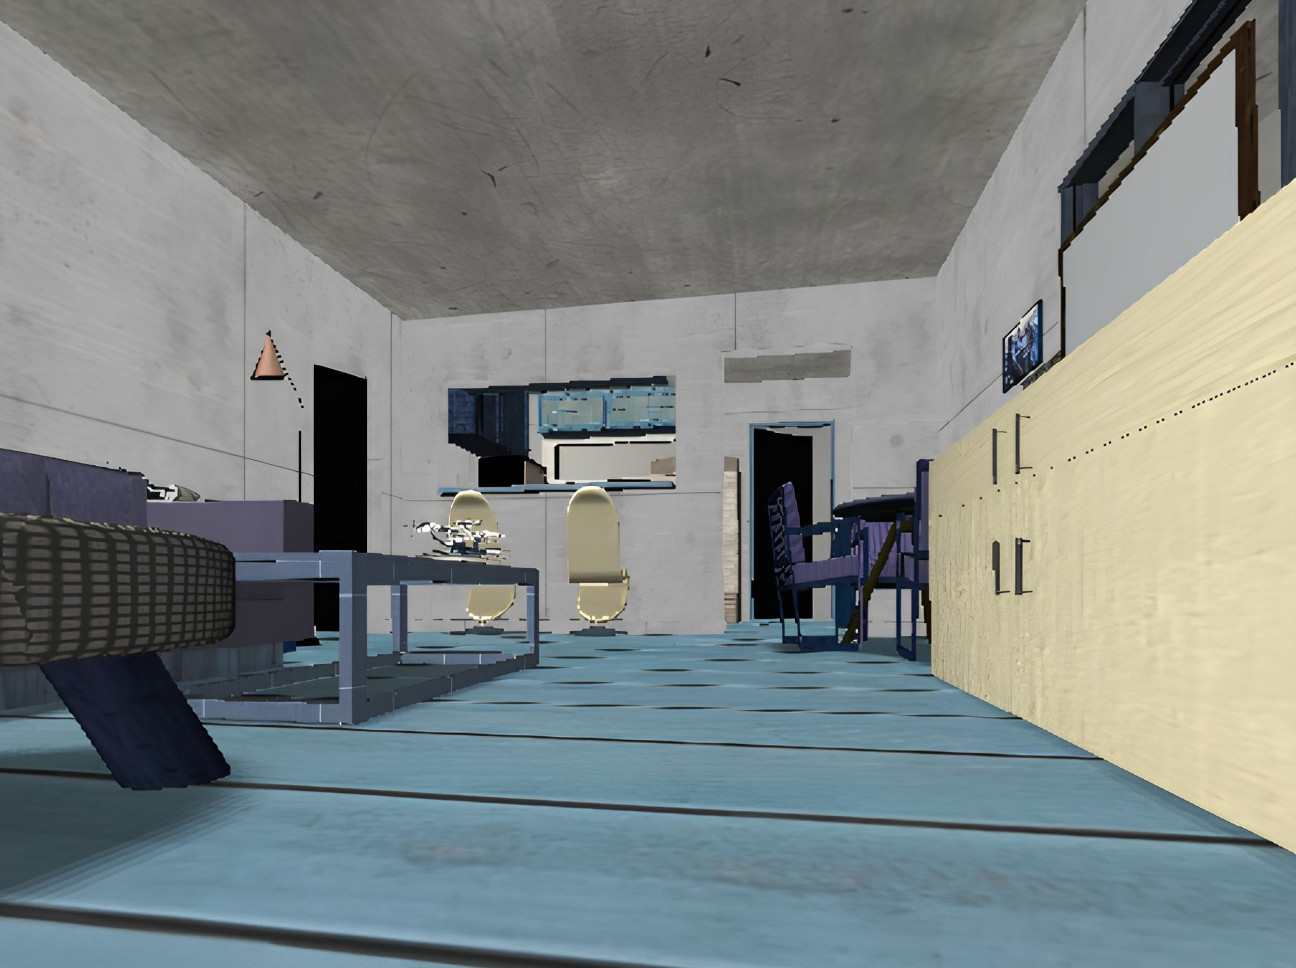
\includegraphics[width=0.38\textwidth]{images/simulated-image.png}}
	\hspace{0.01\textwidth}
	\subfloat[]{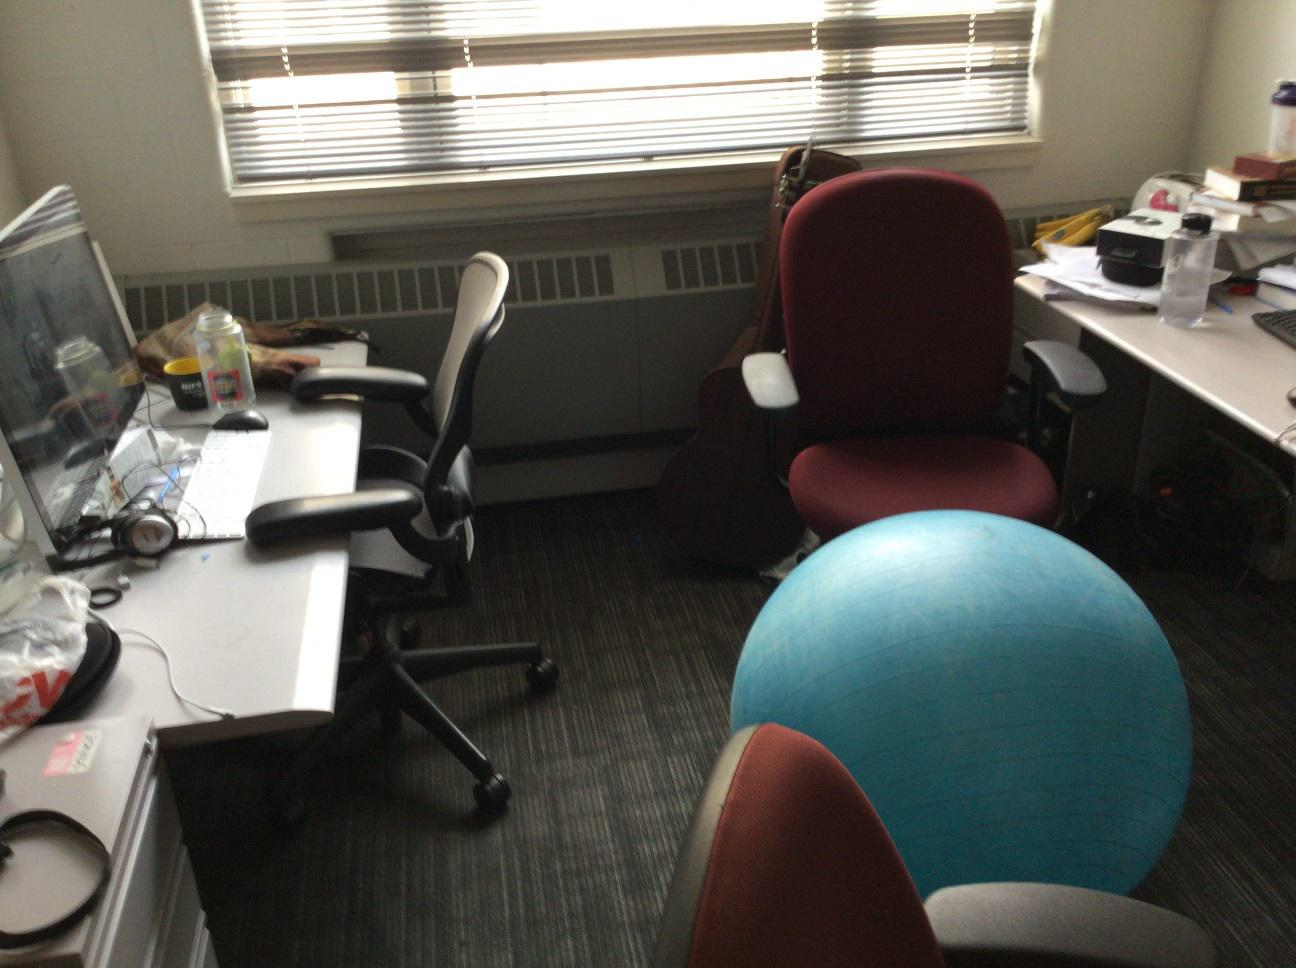
\includegraphics[width=0.38\textwidth]{images/real-image.png}}
	\caption{Immagini raccolte in un ambiente simulato (a) e reale (b).}
	\label{fig:immagine-simulata-reale}
\end{figure}

\section{Domain shift}
\label{sec:domain_shift}

Nella pratica, reti naurali addestrate con dati sintetici e testate in ambienti reali avranno performance scadenti, non riuscendo neanche a riconoscere le categorie di oggetti più comuni presenti nel mondo reale~\cite{8793591}. Questo problema è noto come \textit{sim-to-real gap}, letteralmente \textit{divario tra simulazione e realtà}, e rappresenta la differenza di prestazioni tra un modello addestrato in un ambiente simulato, e le performance nel mondo reale.

Il sim-to-real gap non è però l'unico tipo di domain shift esistente. Si osservano infatti cali di performance anche quando un modello addestrato in ambienti simulati viene testato in altri ambienti simulati (\textit{sim-to-sim gap}), così come si ha una diminuzione di performance in scenari reali, passando da un ambiente reale ad un altro (\textit{real-to-real gap}).

Per il domain shift tra ambienti simulati va innanzitutto fatta una distinzione. Si ha un dominio differente sia tra ambienti diversi all'interno di uno stesso simulatore, sia tra ambienti appartenenti a simulatori differenti. Nel caso di uno stesso simulatore, il domain shift è principalmente causato da variazioni di caratteristiche ambientali e dalle diverse configurazioni degli scenari. Differenze nell'illuminazione, nella disposizione degli oggetti o nella scelta delle texture possono portare a dataset significativamente differenti. Nel caso invece di simulatori diversi, il domain shift diventa ancora più pronunciato. Ogni simulatore utilizza motori grafici differenti, e lo stesso vale per le librerie di oggetti 3D e gli ambienti. Ad esempio simulatori più fotorealistici come AI2-THOR~\cite{kolve2022ai2thorinteractive3denvironment} produrranno immagini con caratteristiche visive differenti rispetto ad uno focalizzato sulla simulazione fisica come DoorGym~\cite{urakami2022doorgymscalabledooropening}. Quindi, senza un'opportuna riconfigurazione o fine tuning, il trasferimento di un modello da un simulatore ad un altro risulta complicato.

Per quanto riguarda il real-to-real gap, le differenze tra diversi ambienti reali sono più marcate rispetto a quelle tra due simulatori. Illuminazione variabile, ostacoli mobili, diversa qualità dei sensori o variazioni nell'arredamento possono degradare notevolmente le performance di un modello addestrato in un particolare ambiente. Ad esempio, un robot addestrato in un ufficio con illuminazione a LED tende a fallire nel riconoscere oggetti in un ambiente domestico con luce naturale, nonostante siano entrambi ambienti reali.


\section{Fog robotics}
\label{sec:fog_robotics}

La fog robotics è un'estensione del concetto di \textit{fog computing}~\cite{10.1145/2757384.2757397} applicato alla robotica mobile, ed è nata per superare il limite delle più tradizionali tecnologie basate sul \textit{cloud computing}~\cite{qian2009cloud}. Questo modello distribuito permette di bilanciare il carico computazionale, la latenza e l'affidabilità, distribuendo il carico di lavoro tra i vari nodi di rete. Questo garantisce risposte in tempo reale per le attività più critiche, come la navigazione e le interazioni con l'ambiente.

Come illustrato nella \hyperref[fig:fog_robotics]{Figura \ref{fig:fog_robotics}}, l'architettura si basa su tre elementi principali:

\begin{figure}[t]
	\centering
	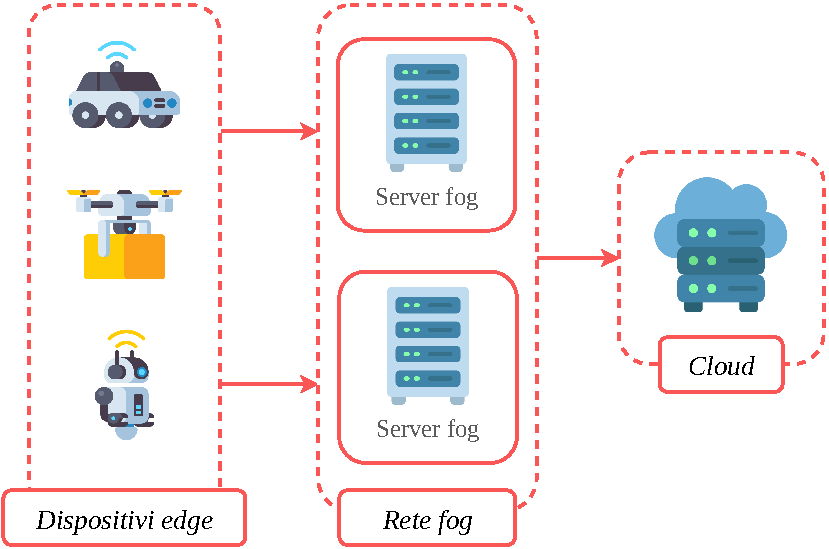
\includegraphics[width=0.8\textwidth, clip]{images/fog-robotics}
	\caption{Schema generale di un'architettura fog robotics.}
	\label{fig:fog_robotics}
\end{figure}

\begin{itemize}
	\item \textbf{Dispositivi edge}: Includono i robot di servizio stessi, dotati di hardware limitato per l'elaborazione dei dati che richiedono una latenza minima. Degli esempi sono il controllo dei motori o le operazioni di sicurezza più critiche, come l'analisi dei dati provenienti dai sensori di profondità. Tutte le altre attività vengono affidate ai livelli più alti.
	
	\item \textbf{Server fog}: Sono nodi di calcolo posizionati geograficamente vicino ai robot, tipicamente server locali che si occupano di eseguire operazioni complesse e con latenze ridotte. La distanza ravvicinata permette infatti di mantenere la latenza nell'ordine dei millisecondi.
	
	\item \textbf{Cloud}: È un'infrastruttira con una maggior potenza di calcolo, utilizzata generalmente per l'elaborazione di dati non time-sensitive e per l'archiviazione di informazioni a lungo termine.
\end{itemize}

Nonostante i suoi vantaggi, l'utilizzo di un'architettura distribuita come questa introduce ulteriori sfide legate al domain shift. Questo avviene a causa dell'eterogeneità dell'hardware presente nei robot e dalla necessità di sviluppare sistemi di visione robotica modulari, in grado di funzionare su più server differenti e senza perdita di prestazioni.

\section{Scopo dell'elaborato}
\label{sec:scopo_dell_elaborato}

L'obiettivo di questo elaborato è studiare il fenomeno del domain shift, analizzando in particolare come le performance di un modello calano nei tre casi precedentemente descritti: sim-to-sim (nel caso di ambienti in uno stesso simulatore), real-to-real e sim-to-real. Oltre a questa analisi, viene presentata e testata un'architettura alternativa progettata per mitigare il problema del domain shift in un sistema distribuito di tipo fog robotics.

% CAPITOLO 2: Stato dell'Arte
\chapter{Stato dell'arte}
\label{chap:stato_arte}

In questo capitolo vengono analizzate le principali tecniche attualmente più utilizzate per affrontare il problema del domain shift. In particolare verranno approfonditi gli approcci di \textit{domain adaptation}, \textit{data augmentation} e \textit{domain randomization}. Infine, il capitolo si sofferma sulle principali innovazioni avvenute nel campo della fog e cloud robotics.

\section{Domain adaptation}
\label{sec:adaptation}

La domain adaptation è una delle strategie più utilizzate per ridurre il domain shift. Questo approccio mira a minimizzare le differenze tra il dominio di origine e quello di destinazione, tramite trasformazioni dei dati o l'adattamento dei modelli. Una tecnica comprende l'utilizzo di tecnologie come le reti generative avversarie (GAN, Generative Adversarial Network)~\cite{10.1145/3422622}, che utilizzano in genere due diverse reti neurali per migliorare la qualità dei dati. Una rete crea nuovi dati con caratteristiche simili a quelle del dominio target, e l'altra valuta la loro somiglianza con i dati reali. Questo approccio si è rivelato particolarmente efficace e ha permesso di migliorare le performance di generalizzazione nei modelli di robotic vision~\cite{Shrivastava_2017_CVPR}.

Uno dei casi più analizzati in letteratura è quello del sim-to-real, nel quale si cerca di trasformare i dati provenienti da un simulatore in immagini simili a quelle reali. Ad esempio, un'immagine presa da un ambiente simulato, con texture uniformi e un'illuminazione predefinita, può essere trasformata in una più fotorealistica variando la luce, aggiungendo riflessi o creando imperfezioni sulla superficie degli oggetti. In pratica si cerca di aggiungere caratteristiche presenti nel mondo reale a dati campionati da simulatori, in modo da ridurre la differenza tra quello che è il dominio della simulazione e quello della realtà.

\section{Data augmentation}
\label{sec:augmentation}

La data augmentation rappresenta un'altra tecnica ampiamente utilizzata per ridurre il domain shift. Consiste nell'applicare trasformazioni ai dataset con l'obiettivo di aumentare sia il numero di dati disponibili, che l'eterogeneità dei dati stessi~\cite{Shorten2019}. Queste trasformazioni possono comprendere rotazioni, ridimensionamenti, traslazioni, e l'applicazione di filtri che possano simulare condizioni ambientali come nebbia, riflessi e occlusione ambientale. La data augmentation permette sia di aumentare la dimensione di dataset senza la necessità di campionare nuovi dati, sia consente ai modelli di generalizzare meglio alle variazioni presenti nel mondo reale. Degli esempi di trasformazioni sono visibili nella \hyperref[fig:immagine-augmentata]{Figura \ref{fig:immagine-augmentata}}. Consideriamo ad esempio un robot che deve riuscire a riconoscere e classificare oggetti in ambienti con un'illuminazione dinamica; applicare filtri per simulare differenti condizioni di luce può migliorare significativamente le sue abilità di generalizzazione~\cite{NEURIPS2021_fb4c4860}. Inoltre, la data augmentation può essere usata in presenza di dataset sbilanciati, nei quali alcune classi sono sottorappresentate rispetto ad altre. Attraverso una serie di trasformazioni è infatti possibile aumentare il numero di dati appartenenti alle classi meno presenti, migliorando di conseguenta le capacità del modello nel riconoscerle.

\begin{figure}[t]
	\centering
	\subfloat[]{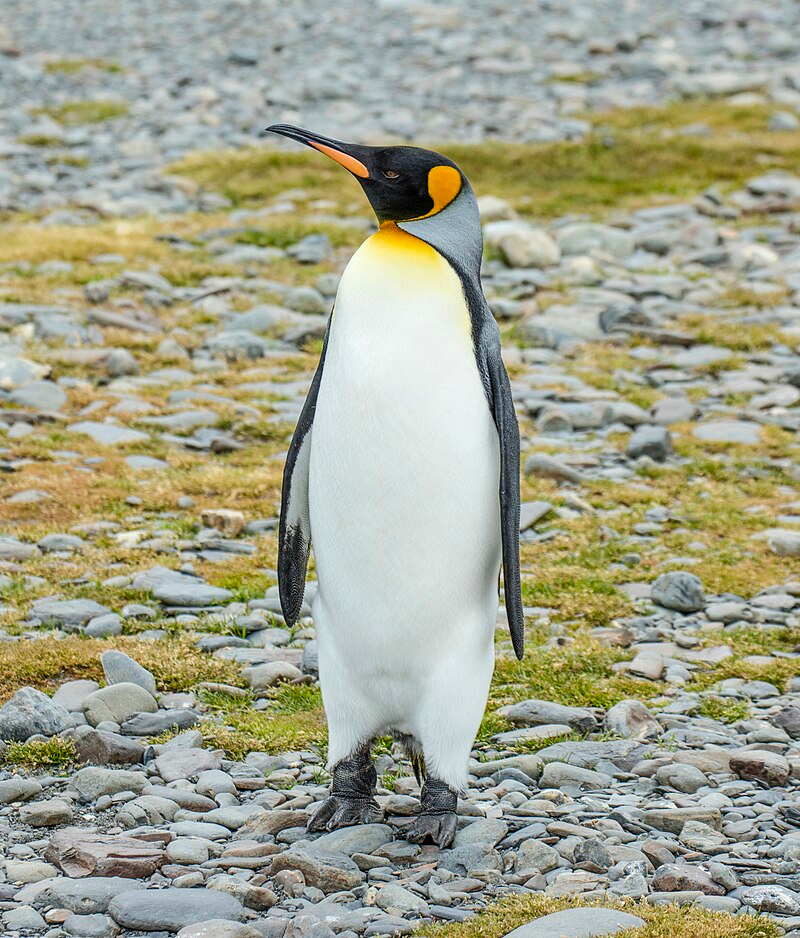
\includegraphics[width=0.23\textwidth]{images/penguin-original.png}}
	\hspace{0.01\textwidth}
	\subfloat[]{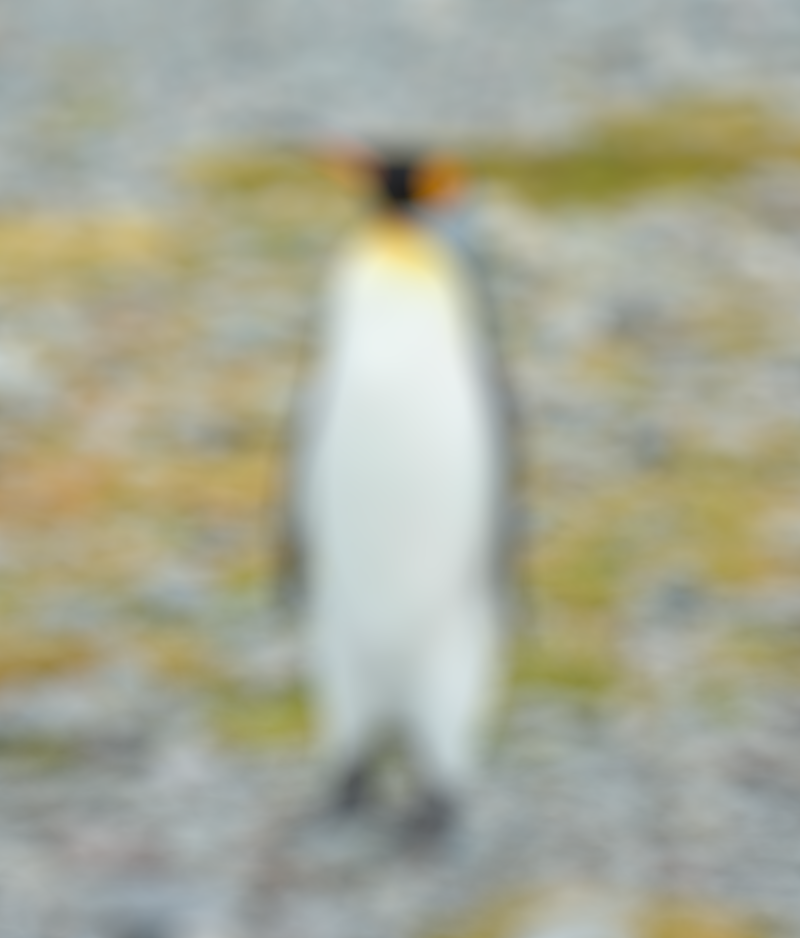
\includegraphics[width=0.23\textwidth]{images/penguin-blur.png}}
	\hspace{0.01\textwidth}
	\subfloat[]{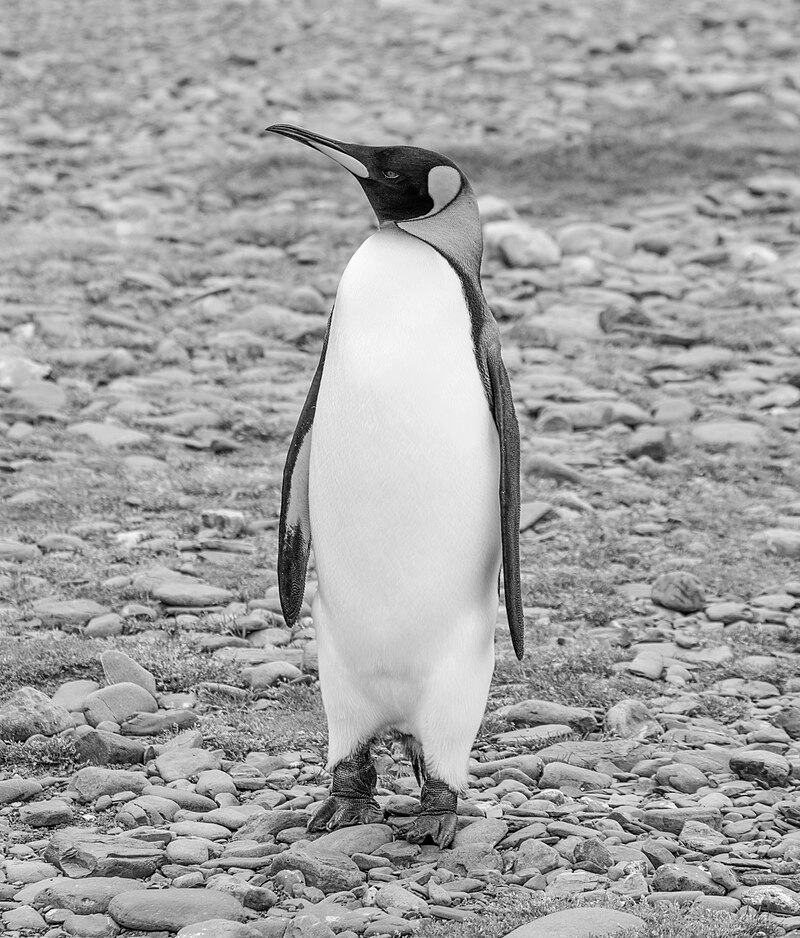
\includegraphics[width=0.23\textwidth]{images/penguin-black-and-white.png}}
	\hspace{0.01\textwidth}
	\\	
	\subfloat[]{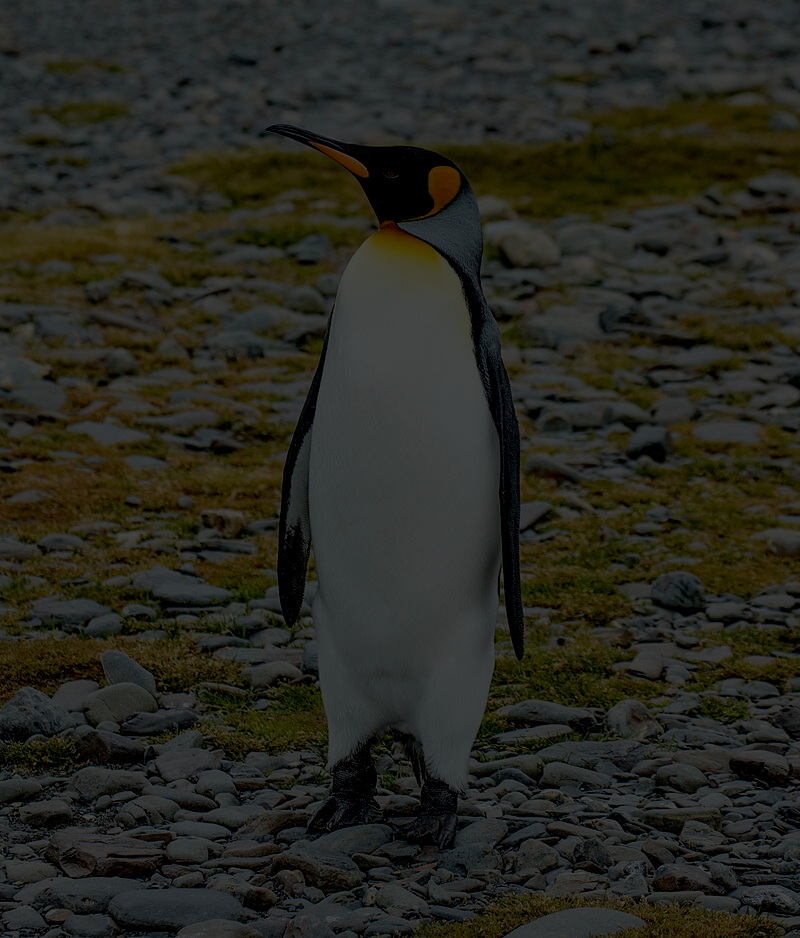
\includegraphics[width=0.23\textwidth]{images/penguin-low-exposure.png}}
	\hspace{0.01\textwidth}
	\subfloat[]{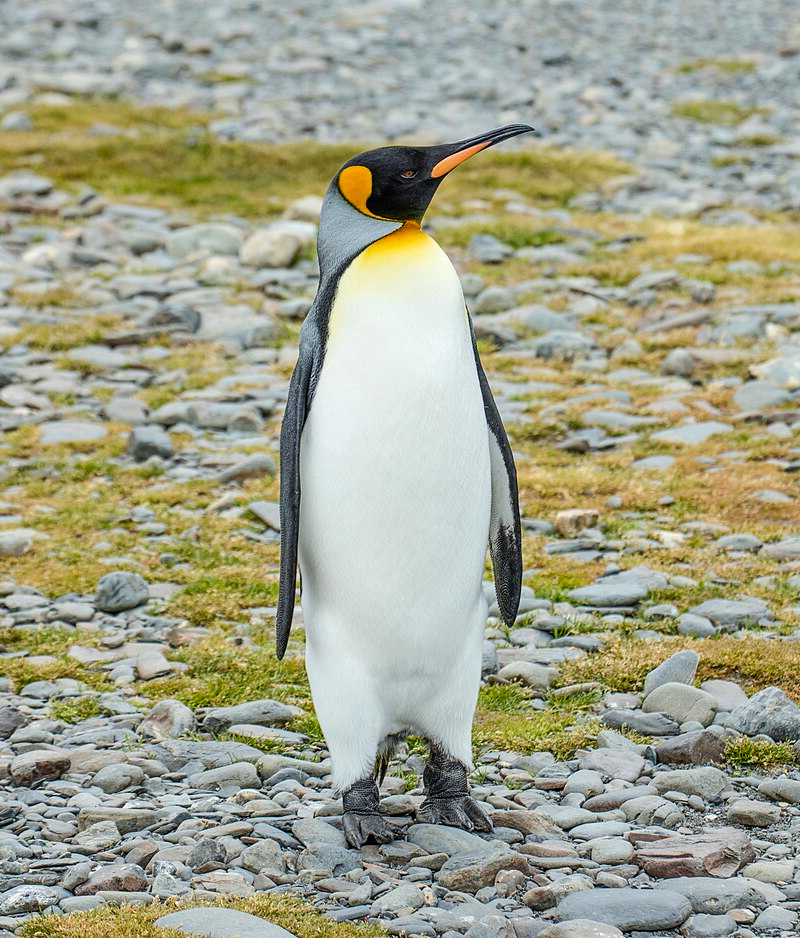
\includegraphics[width=0.23\textwidth]{images/penguin-flip.png}}
	\hspace{0.01\textwidth}
	\subfloat[]{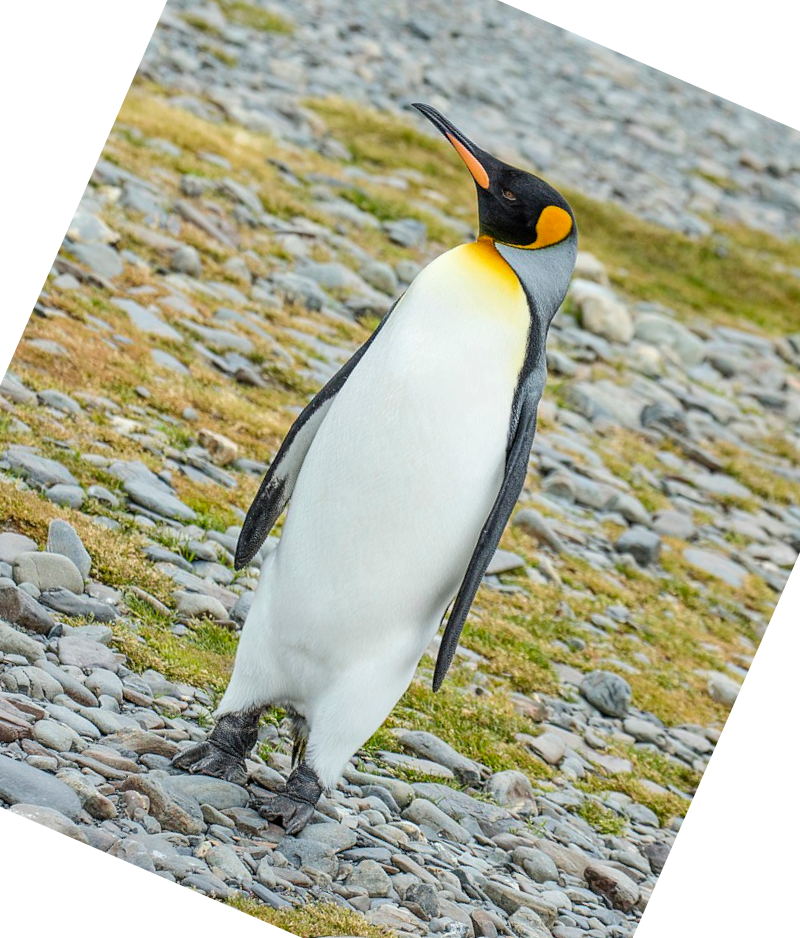
\includegraphics[width=0.23\textwidth]{images/penguin-rotation.png}}
	\caption{Esempio di trasformazioni applicate ad un'immagine. Rispettivamente l'immagine originale (a), sfocata (b), in bianco e nero (c), a bassa esposizione (d), specchiata (e) e ruotata (f).}
	\label{fig:immagine-augmentata}
\end{figure}

Un'altro esempio nel quale questa tecnica può tornare utile, è nel caso si vengano a creare dipendenze da caretteristiche non rilevanti (bias). Ad esempio, se un modello tende ad associare la presenza di uno specifico sfondo a quella di un particolare oggetto, può essere conveniente effettuare trasformazioni andando a modificare o rimuovere lo sfondo, in modo da rendere indipendente la presenza di un oggetto da quella di un'altro.

Un esempio di bias è ben descritto nell'articolo~\cite{diagnostics12010040}, relativo ad un modello addestrato a riconoscere melanomi da tessuti sani. La rete neurale è stata addestrata a partire da un dataset contenente foto raffiguranti tumori maligni e tessuti epiteliali sani. Sebbene i risultati di validazione fossero inizialmente promettenti, si è scoperto che il modello non aveva realmente imparato a riconoscere la presenza di melanomi. Piuttosto, basava le sue previsioni su correlazioni spurie presenti nei dati. Nelle immagini raffiguranti tessuti sani erano sempre presenti strumenti come righelli e altri dispositivi per la calibrazione, che erano invece assenti in quelle rappresentanti tumori maligni. Come conseguenza, questi dati hanno portato il modello a trovare delle scorciatoie (\textit{shortcut learning}), utilizzando la presenza di questi artefatti come principale regola per classificare le immagini.

\section{Domain randomization}
\label{sec:randomization}

La domain randomization~\cite{8202133} risulta particolarmente utile quando si devono campionare dati da un ambiente simulato. Invece che raccogliere dati da una singola scena statica, la domain randomization permette di randomizzare gli elementi come oggetti, luce, texture ed eventuale rumore in maniera automatica all'interno di uno stesso ambiente. Questo consente al modello di imparare molteplici dispozizioni di oggetti e caratteristiche, migliorandone così le capacità di generalizzazione. Con questo approccio si cercano quindi di ricreare le condizioni che caratterizzano un normale ambiente domestico; a distanza di pochi giorni è raro che vengano introdotti o rimossi degli oggetti, mentre è molto più probabile che oggetti già presenti vengano spostati. Questo comporta una diversa disposizione degli oggetti, con una conseguente differenza nell'illuminazione della stanza, nei riflessi, e possibilmente anche nei colori. Se il modello non è abbastanza robusto a questo tipo di cambiamenti, potrebbe non riuscire a generalizzare correttamente.

Questa tecnica è particolarmente efficace nell'addestrare reti neurali profonde (DNN, Deep Neural Netework) per compiti come l'identificazione e la manipolazione di oggetti. Ha infatti permesso di addestrare un modello utilizzando solo immagini simulate, riuscendo poi a localizzare in maniera accurata oggetti in ambienti reali, senza necessitare di ulteriori dati provenienti dal mondo reale.

La domain randomization permette quindi di generare grandi dataset di addestramento col minimo sforzo da parte di un operatore umano, e di ottenere modelli robusti senza la necessità di effettuare fine tuning con dati reali.

\section{Fog e cloud robotics}
\label{sec:fog_e_cloud_robotics}

Le architetture fog robotics sono un'evoluzione delle più tradizionali soluzioni cloud-based, e permettono di bilanciare il carico computazionale e la latenza, andando a migliorare al contempo l'affidabilità. Recenti studi come RoboEC2~\cite{10347007} hanno introdotto nuovi approcci per effettuare \textit{offloading computazionale} in maniera dinamica, andando a migliorare latenza e affidabilità in caso di condizioni di rete variabili. Come il nome può suggerire, questo studio di basa sui servizi Amazon EC2, e implementa un modello che suddivide dinamicamente i livelli di una rete neurale tra edge e cloud. Il tutto trovando un compromesso tra accuratezza, consumo energetico e tempi di elaborazione. In questo lavoro viene anche proposta l'integrazione di un algoritmo chiamato \textit{Spotlight Criteria}, che permette di ottimizzare le decisioni di offloading basandosi su parametri come comsumo computazionale locale, il tempo di risposta e la disponibilità di banda. Questo gli permette di operare anche in condizioni di rete instabili o intermittenti.

Un altro contributo fondamentale è costituito dall'articolo \textit{Cloud Robotics: Architecture, Challenges and Applications}~\cite{6201212}, nel quale vengono proposte architetture ibride di tipo M2M (machine-to-machine) e M2C (machine-to-cloud) e che introduce tre modelli di elastic computing: \textit{peer-based}, \textit{proxy-based} e \textit{clone-based}.

Diversi studi~\cite{9360855} hanno mostrato inoltre come la fog robotics migliori l'efficienza nella gestione delle risorse, consentendo ai robot di operare in ambienti dinamici senza le latenza caratteristiche di un sistema cloud. Ad esempio, nei sistemi multi-robot, l'adozione di server fog locali facilita la coordinazione e l'elaborazione dei dati in loco, riducendo il traffico di rete e il rischio di congestione dei server remoti. Tuttavia, nonostante i vantaggi, la fog robotics introduce nuove sfide, tra cui la gestione dell'eterogeneità sia hardware che software, e la sicurezza della comunicazione tra i vari livelli dell'architettura.

% CAPITOLO 3: Metodo
\chapter{Metodo}
\label{chap:metodo}

Come discusso nel \hyperref[cap:introduzione]{Capitolo \ref{cap:introduzione}}, lo scopo di questo elaborato è analizzare il fenomeno del domain shift in tre scenari differenti, quantificando il calo prestazionale in ciascun caso. Viene inoltre proposta un'architettura per ridurre il domain shift tramite domain adaptation in un contesto distribuito, combinando un segmentatore semantico e un modello di tipo encoder-decoder.

Nel seguente capitolo vengono analizzate le tecnologie e gli strumenti utilizzati, motivandone le scelte e descrivendo il loro impiego all'interno di questo lavoro. Inoltre, vengono descritti i processi di creazione e addestramento dei modelli, presentando frammenti di codice che illustrano l'implementazione.

\section{Task di segmentazione}
\label{sec:task_di_segmentazione}

Prima di iniziare è essenziale capire quali caratteristiche (\textit{feature}) i nostri modelli devono riuscire a rilevare all'interno dell'ambiente. Nel nostro caso si vogliono riconoscere determinate classi di oggetti e individuarne i contorni precisi; ci interessa quindi effettuare un task di segmentazione.

La segmentazione può essere suddivisa in due categorie: semantica e d'istanza. La prima consiste nell'assegnare a ciascun pixel di un'immagine un valore che indica a quale classe appartiene l'oggetto rappresentato da quel pixel. La seconda invece, non solo associa un valore di classe a ciascun pixel, ma identifica in maniera univoca ogni oggetto, consentendo la distinzione tra oggetti appartenenti ad una stessa classe. Un esempio di segmentazione semantica e segmentazione d'istanza è illustrato nella \hyperref[fig:segmentazione]{Figura \ref{fig:segmentazione}}.

\begin{figure}[t]
	\centering
	\subfloat[]{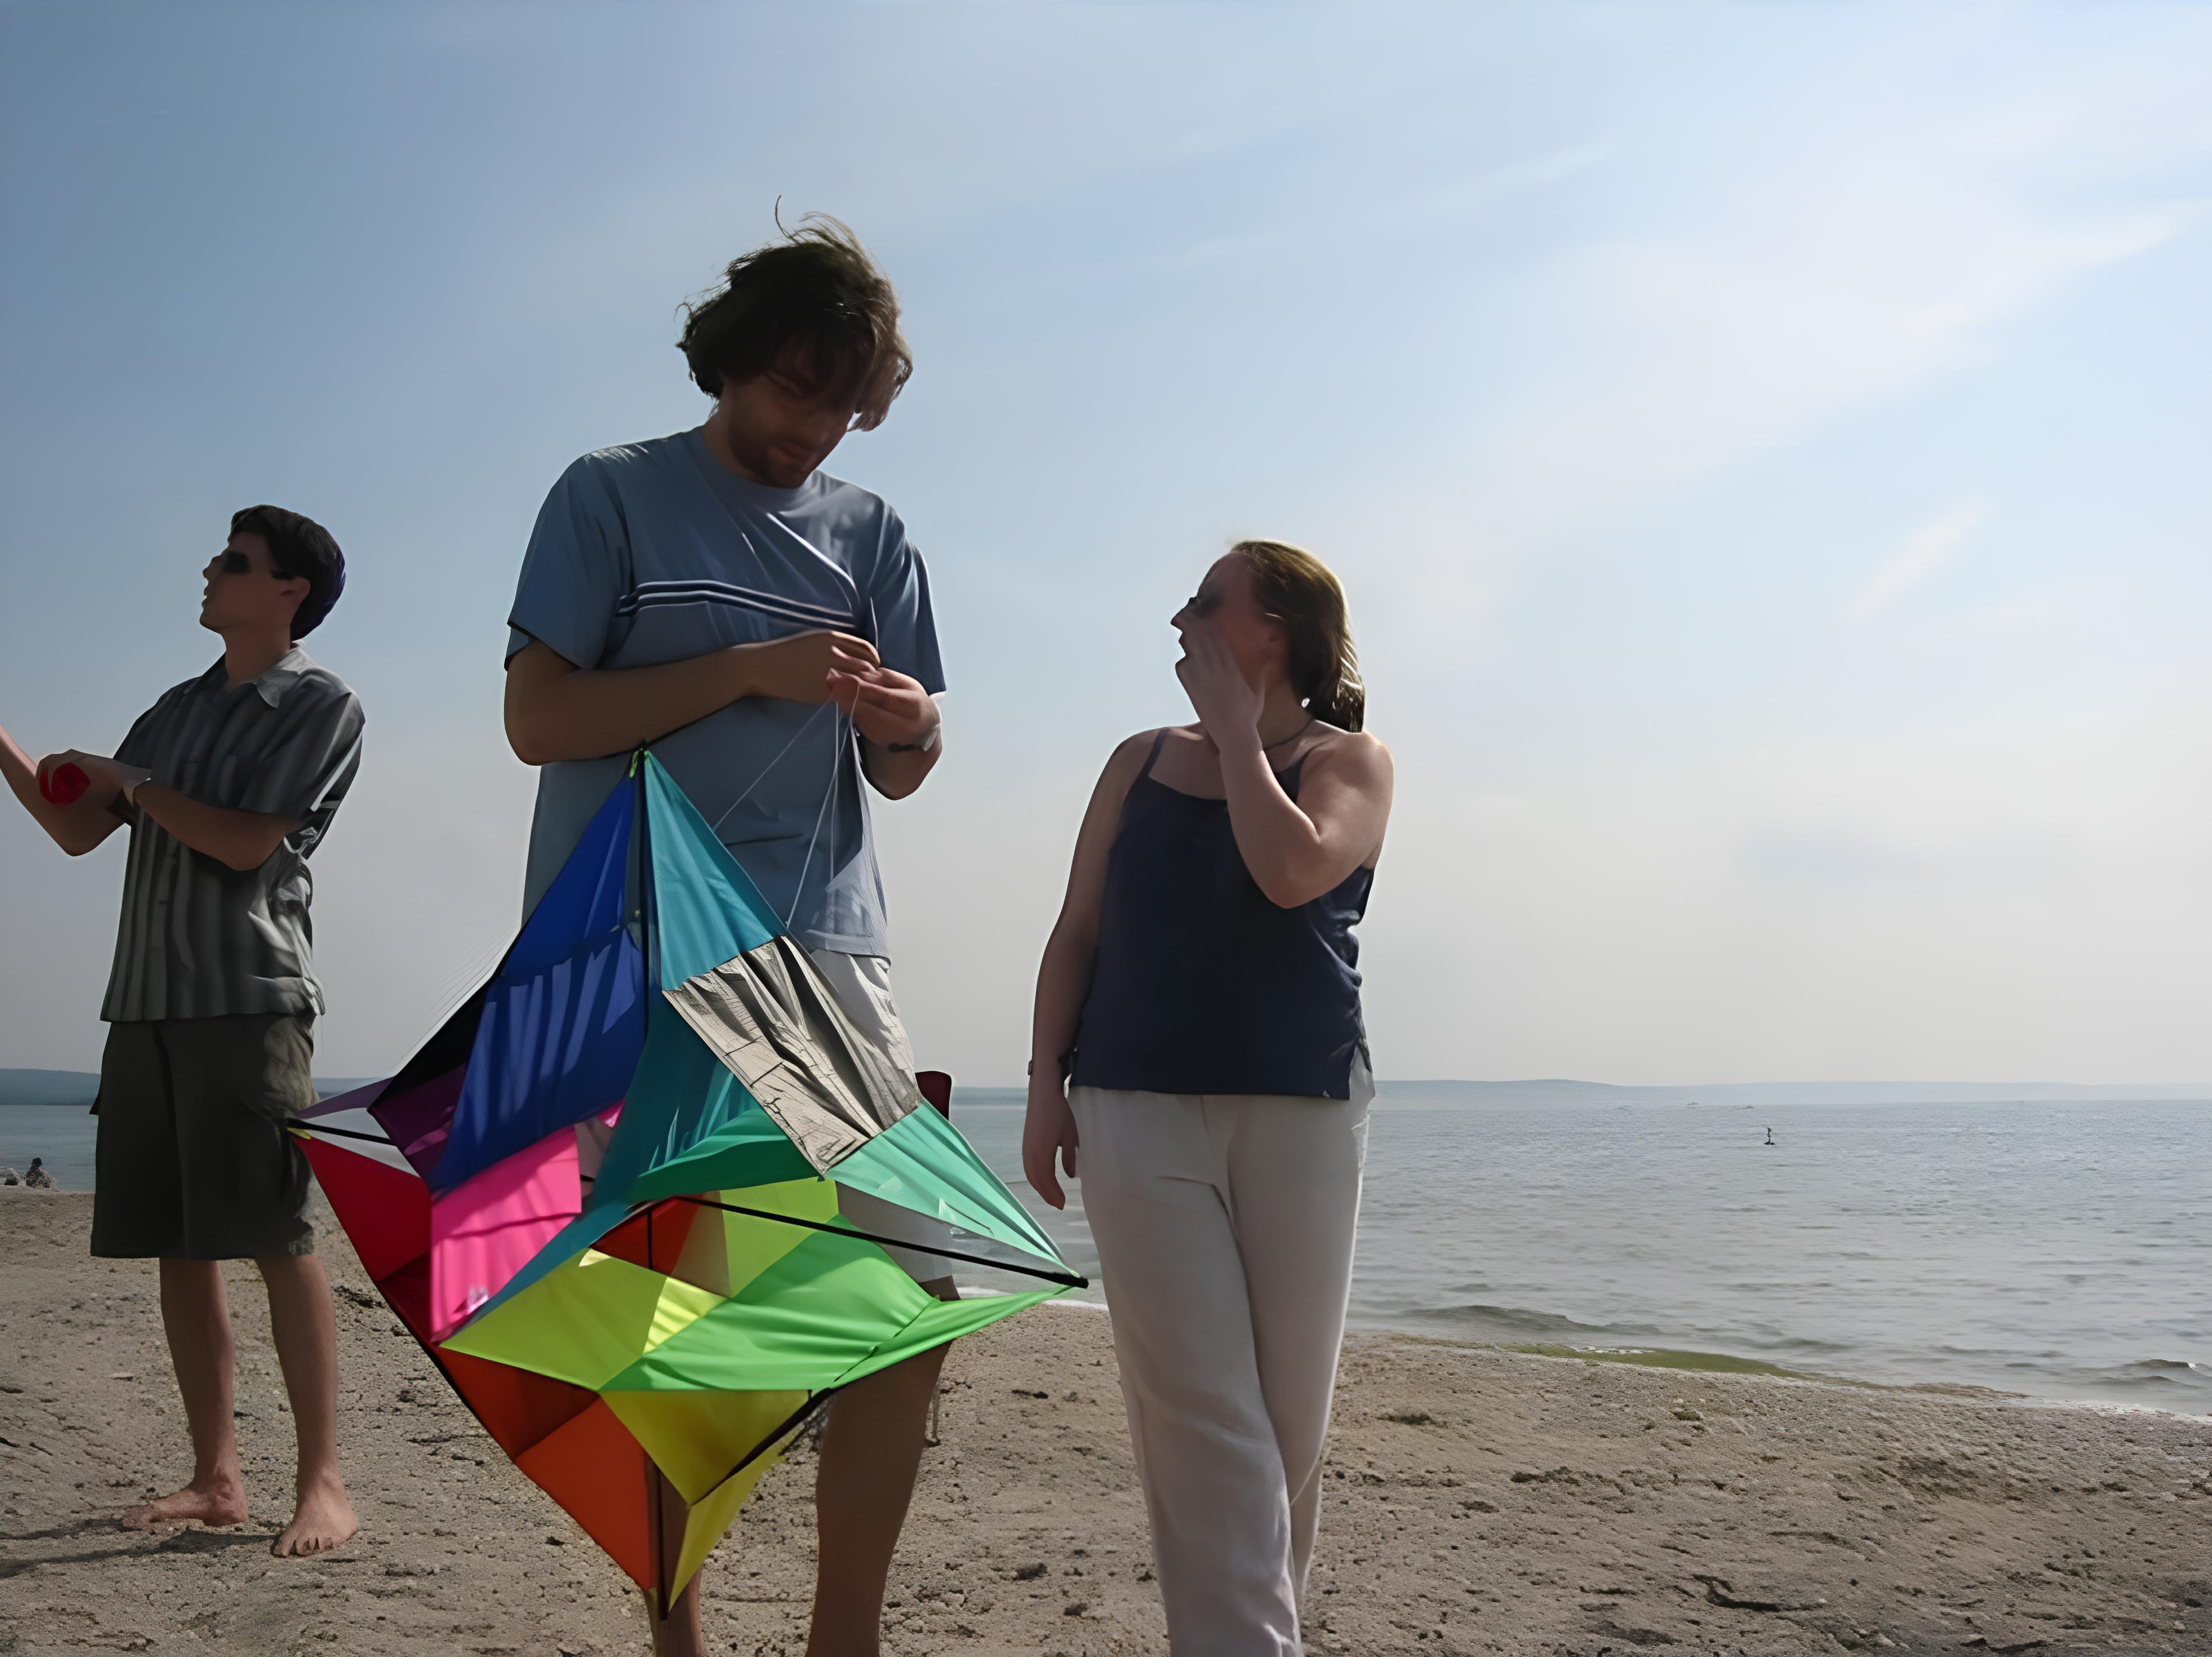
\includegraphics[width=0.23\textwidth]{images/original-segmentation.png}}
	\hspace{0.01\textwidth}
	\subfloat[]{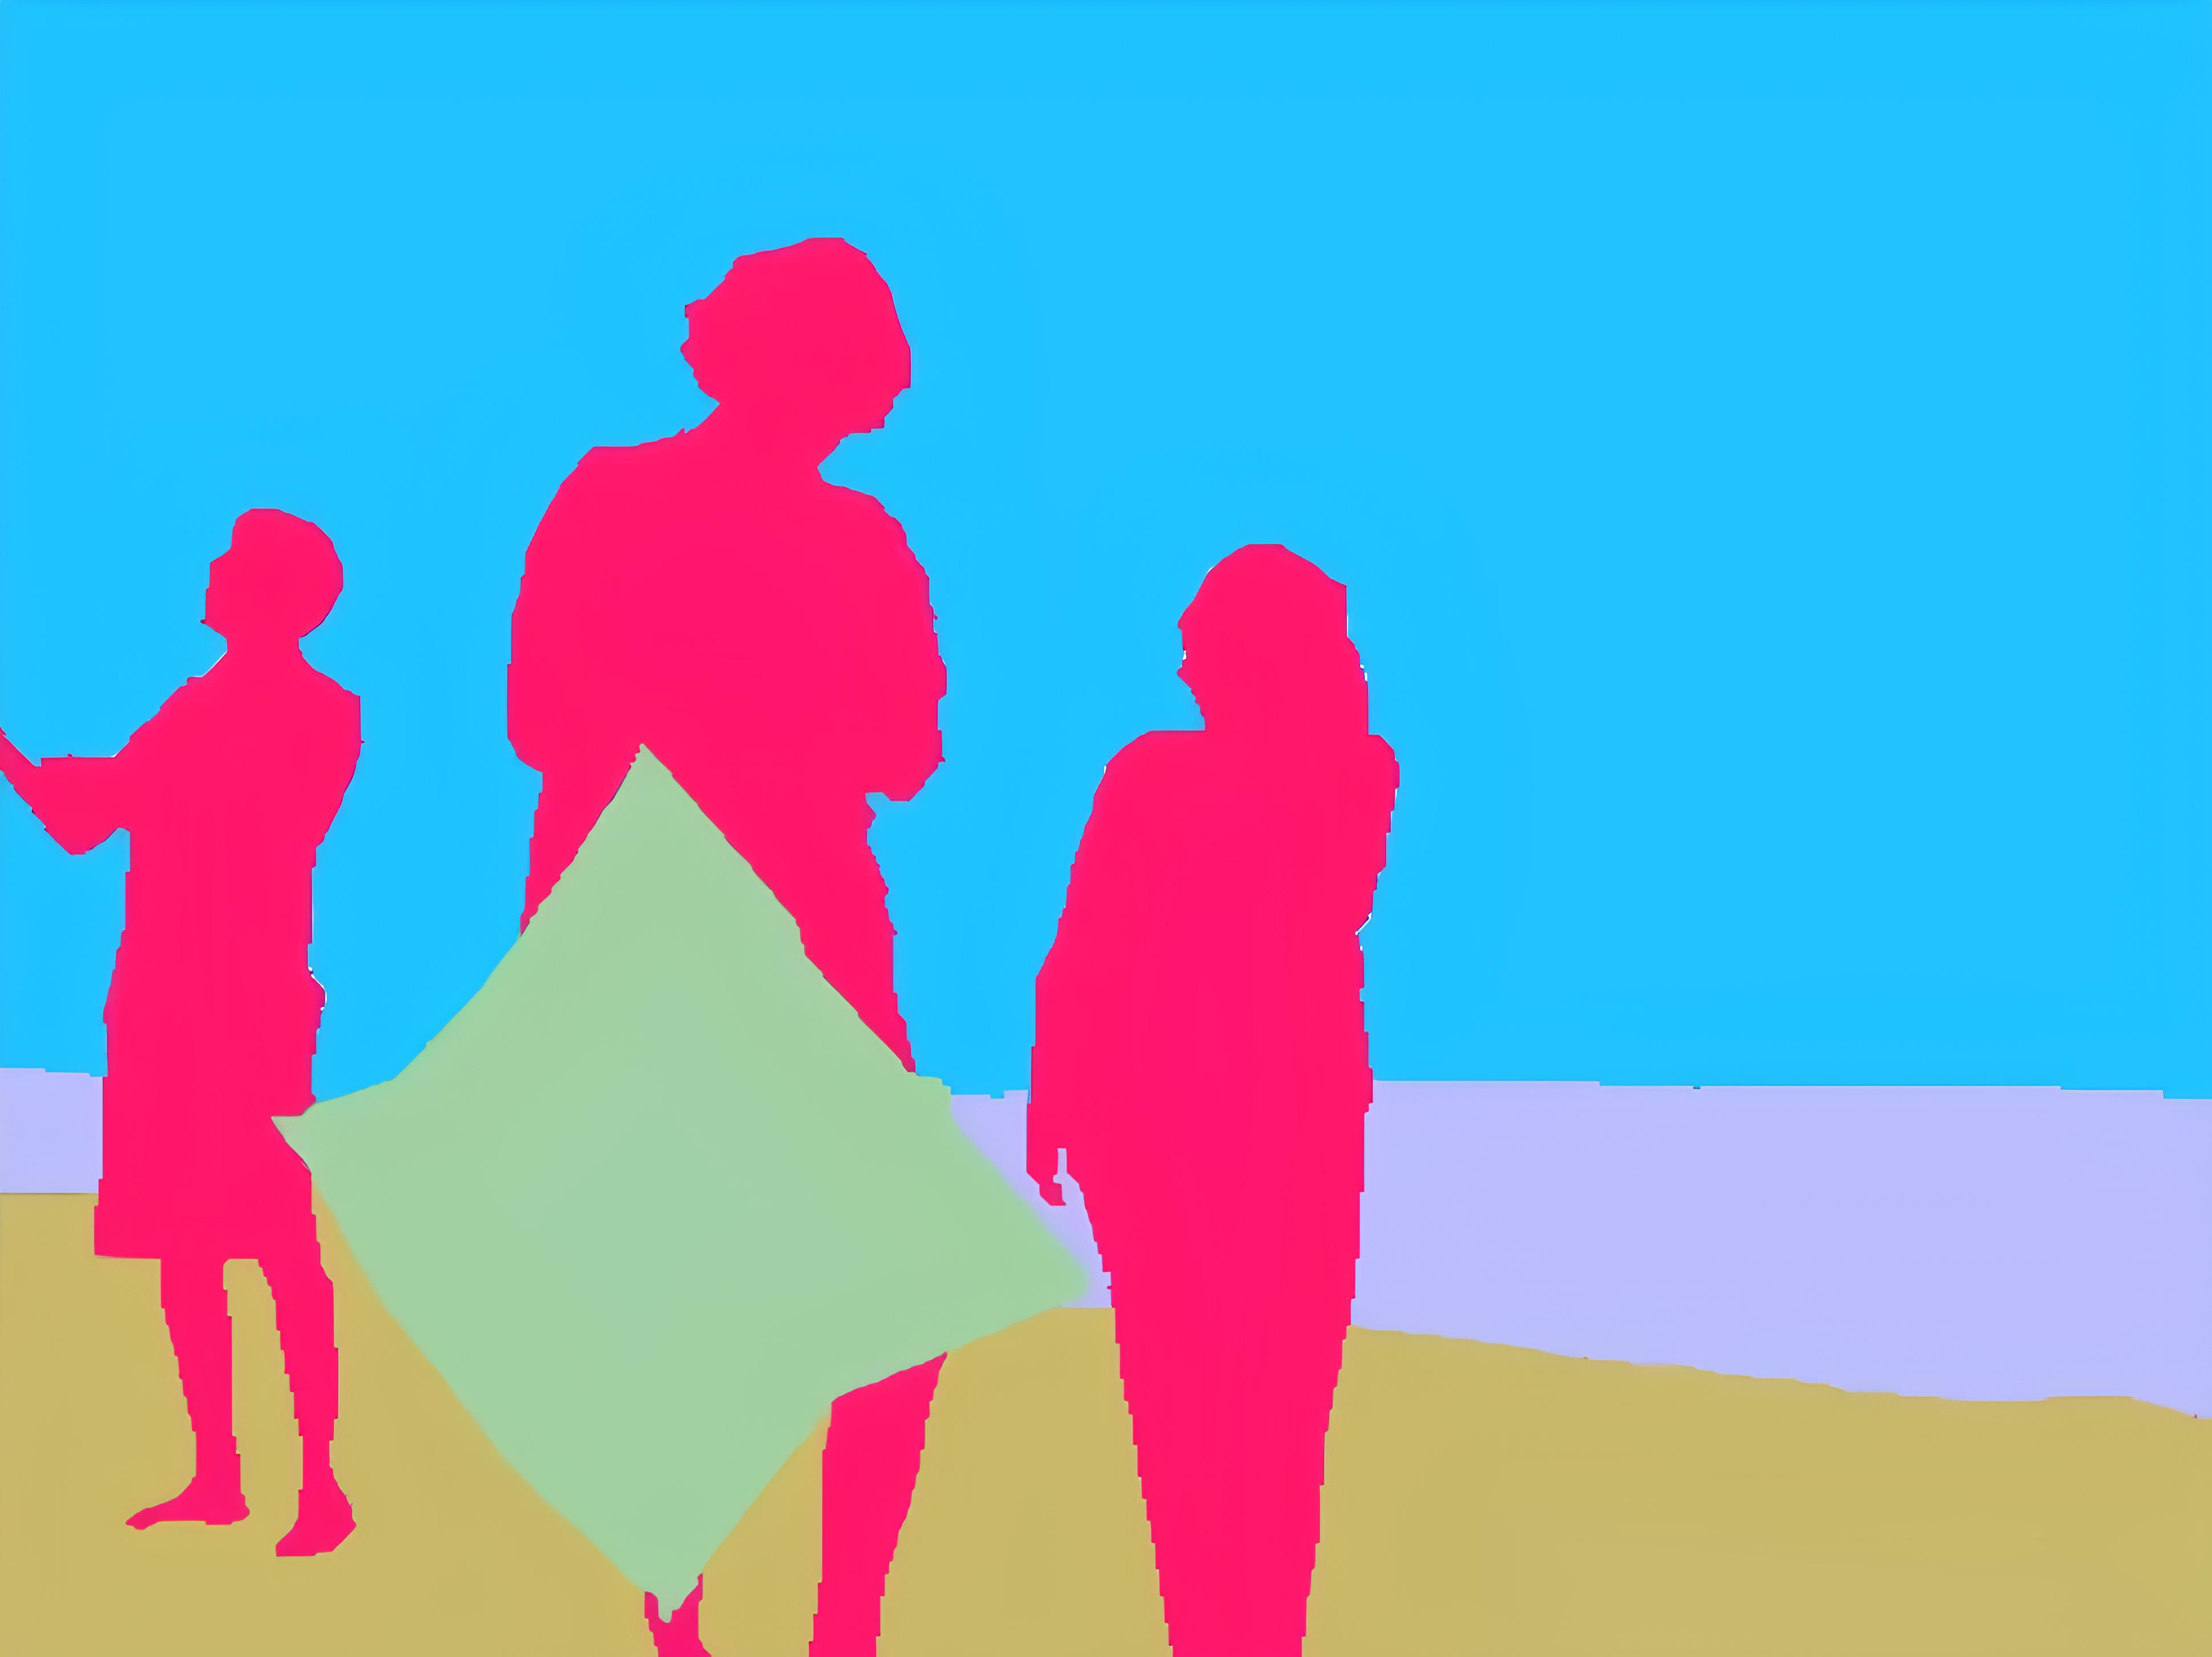
\includegraphics[width=0.23\textwidth]{images/semantic-segmentation.png}}
	\hspace{0.01\textwidth}
	\subfloat[]{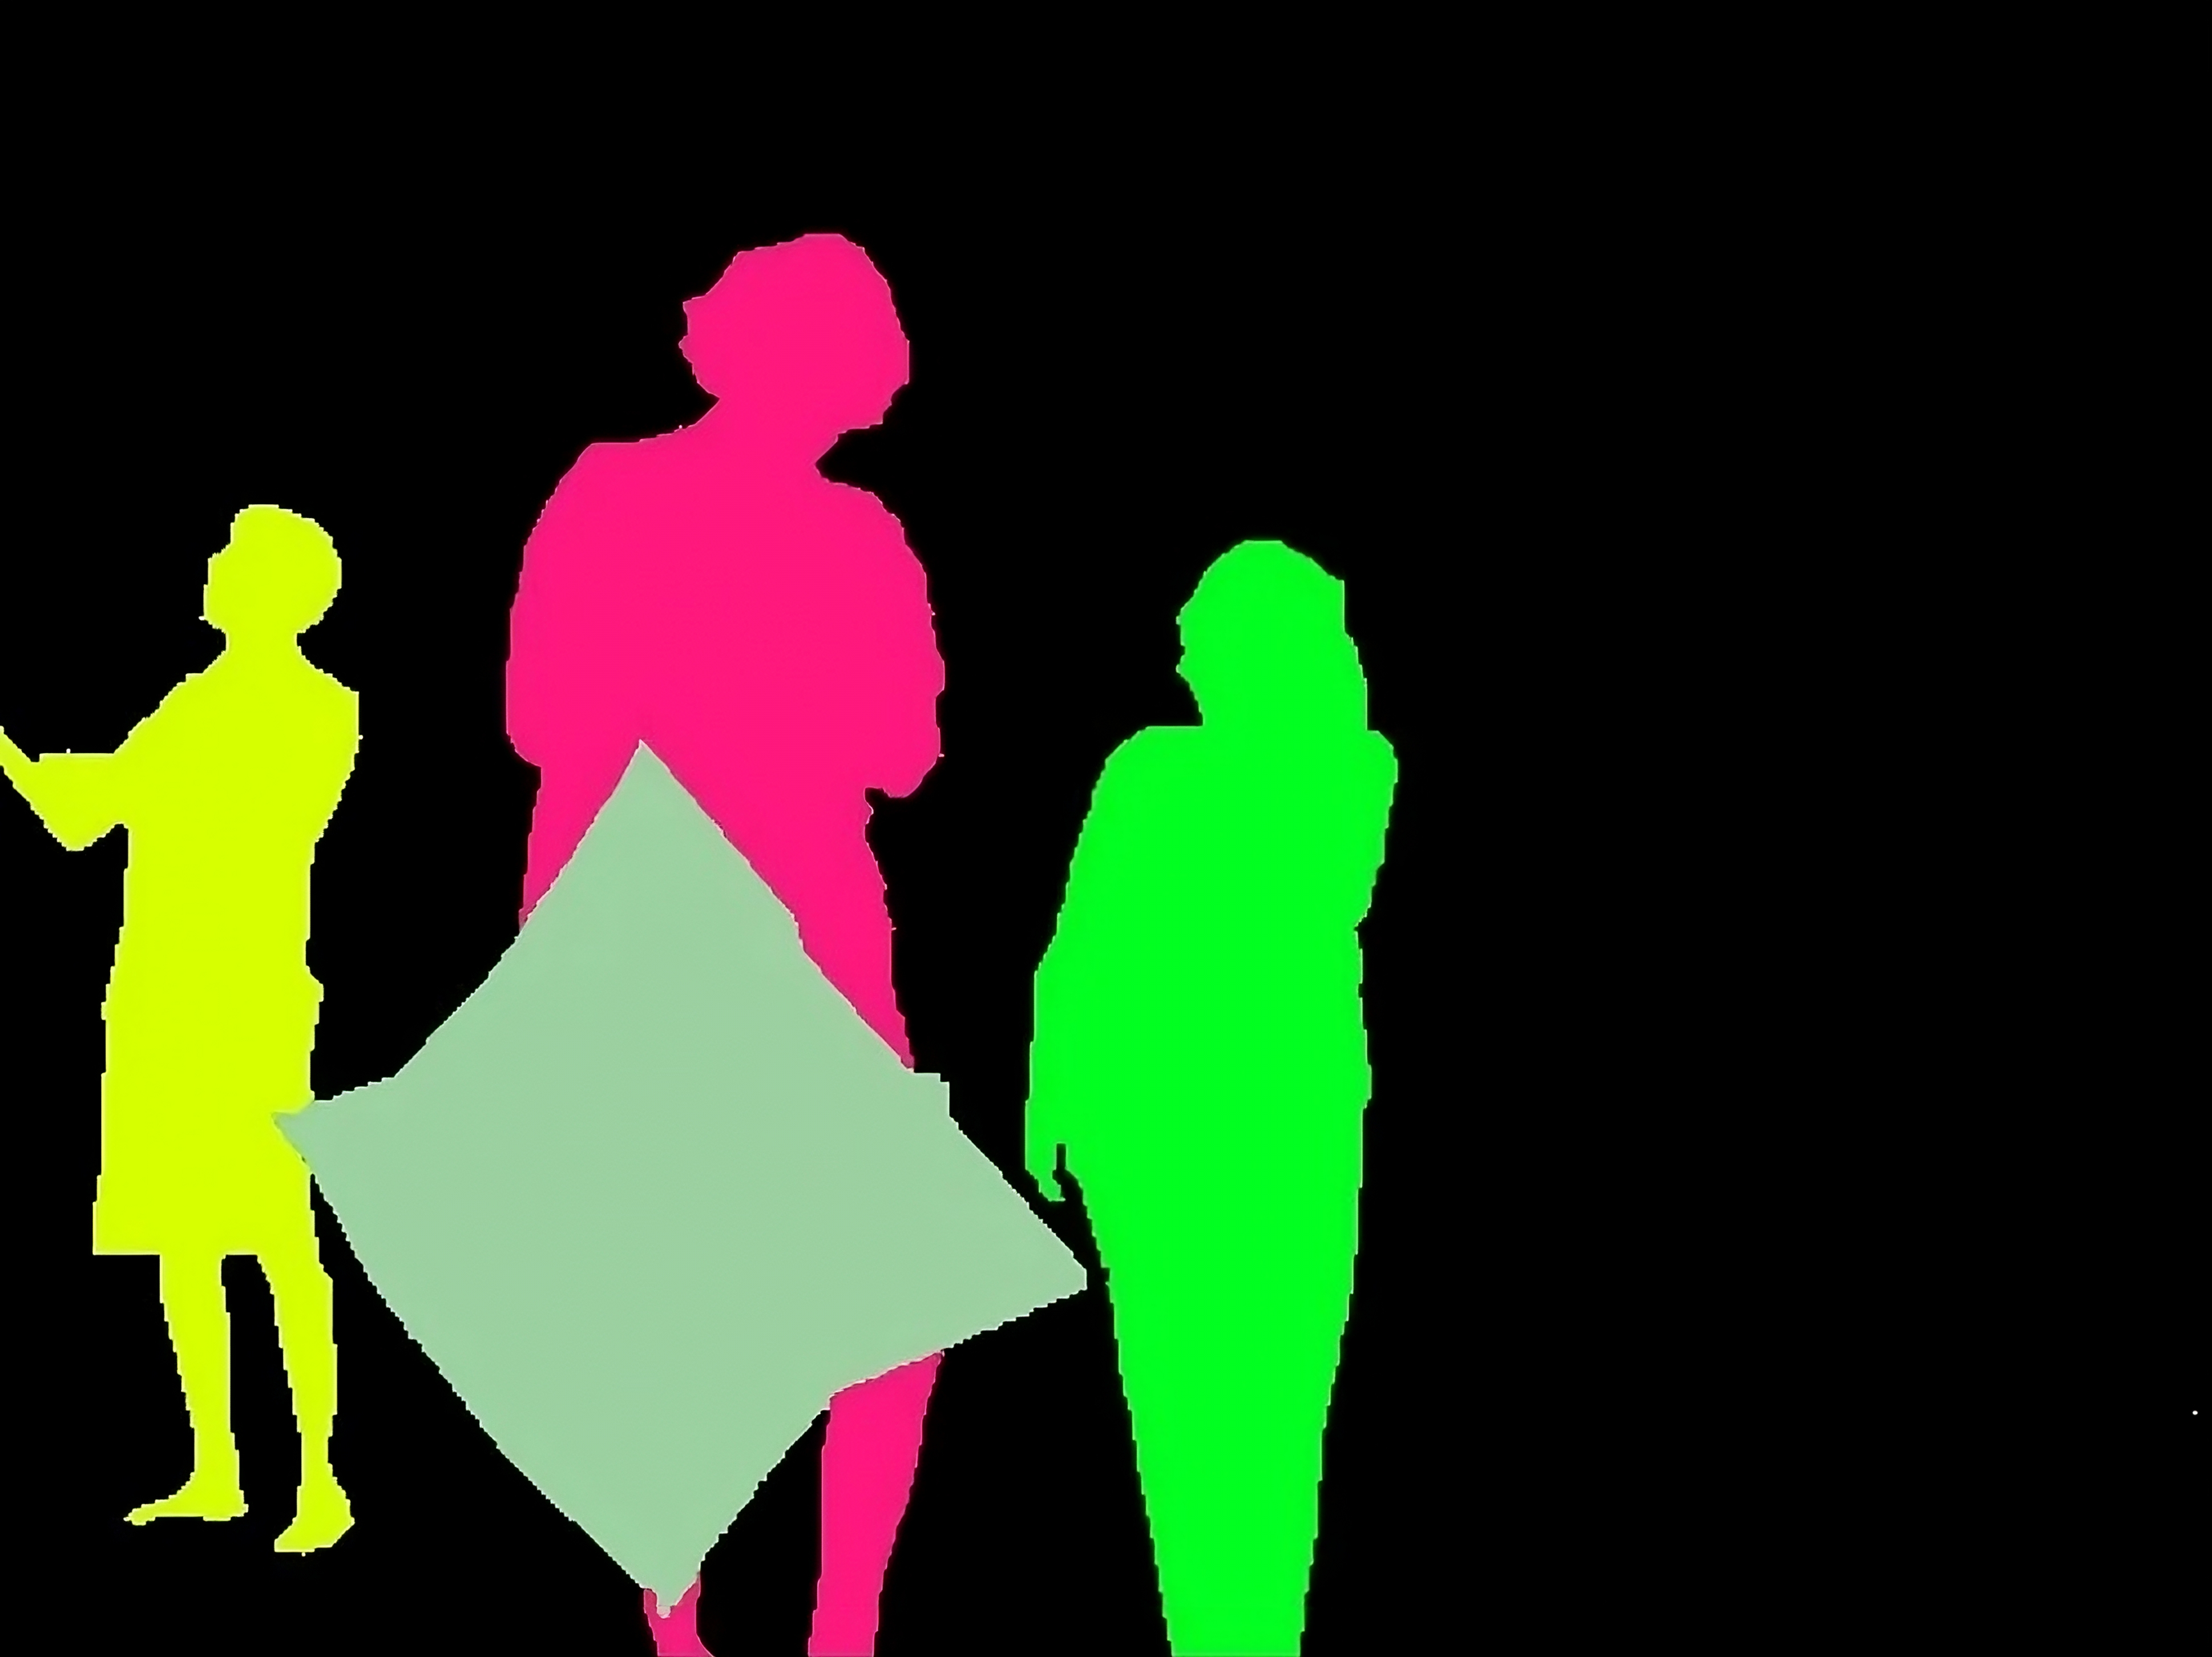
\includegraphics[width=0.23\textwidth]{images/instance-segmentation.png}}
	\caption{Data un'immagine (a), esempio di segmentazione semantica (b) e segmentazione d'istanza (c).}
	\label{fig:segmentazione}
\end{figure}

In questo lavoro si è deciso di adottare la segmentazione semantica, in quanto ci consente di semplificare il lavoro del modello, e di conseguenza ridurne la complessità.

\section{Architettura modello distribuito}
\label{sec:modello_per_fog_robotics}

Mentre l'analisi delle performance nei tre scenari principali (sim-to-sim, real-to-real e sim-to-real) richiede l'utilizzo di una singola rete neurale, il compito di domain adaptation in un sistema distribuito obbliga a riprogettare l'intero modello. Una parte deve essere infatti eseguita sui server fog, mentre l'altra va gestita in cloud. Questi due moduli sono rappresentati da un modello per la trasformazione dei dati (\textit{encoder-decoder}) e uno per la segmentazione semantica (\textit{segmentatore}).

Il nostro obiettivo è trasformare le immagini ricevute in input dall'architettura in altre immagini proiettate sul dominio di addestramento, utilizzando un'architettura di tipo encoder-decoder. Vogliamo quindi rielaborare i dati reali ricevuti in ingresso, e modificarli in modo da farli assomigliare il più possibile a quelli attesi dal segmentatore. L'output dell'encoder-decoder viene poi utilizzato come input del segmentatore, che a questo punto fa inferenza sul dato ricevuto.

Il processo di addestramento di questo modello distribuito è suddiviso in due fasi:

\begin{enumerate}
	\item \textbf{Addestramento del segmentatore}: Inizialmente il segmentatore viene addestrato con dati provenienti dal dominio sorgente. Questo passaggio è essenziale per garantire che il segmentatore apprenda correttamente caratteristiche del dominio di partenza.
	
	\item \textbf{Co-addestramento dell'encoder-decoder e del segmentatore}: Successivamente l'encoder-decoder e il segmentatore vengono co-addestrati con dati provenienti dal dominio di destinazione. In questa fase, i dati passano prima attraverso l'encoder-decoder che cerca di proiettarli sul dominio sorgente, e successivamente vengono dati come input al segmentatore. A questo punto il modello di segmentazione calcola la loss e aggiorna i pesi di entrambi i modelli tramite la funzione di backpropagation. Questo processo consente all'encoder-decoder di imparare a trasformare i dati in maniera efficace, e al contempo il segmentatore si adatta al nuovo dominio tramite processo di \textit{fine-tuning}.
\end{enumerate}

Una criticità di questo approccio è la necessità di disporre di una piccola quantità di dati provenienti dal dominio destinazione, per l'addestramento dell'encoder-decoder. Questa limitazione, nonostante rappresenta un potenziale svantaggio, è significativamente meno onerosa rispetto alla realizzazione di grandi dataset annotati richiesti da altre tecniche. Uno schema riassuntivo dell'architettura proposta è illustrato nella \hyperref[fig:architettura-unet-yolo]{Figura \ref{fig:architettura-unet-yolo}}.

\begin{figure}[t]
	\centering
	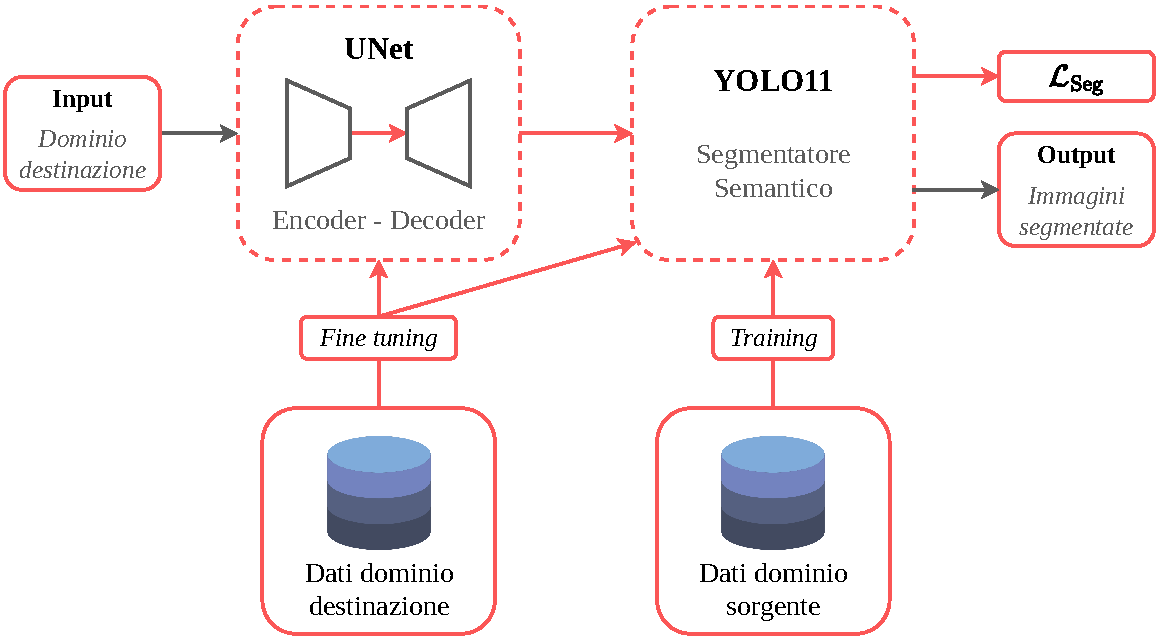
\includegraphics[width=\textwidth, clip]{images/unet-yolo-architecture}
	\caption{Architettura del modello distribuito.}
	\label{fig:architettura-unet-yolo}
\end{figure}

\section{Strumenti}
\label{sec:strumenti}

In questa sezione verranno descritti i diversi strumenti utilizzati in questo elaborato per implementare l'architettura proposta. La scelta di ciascuno strumento è stata guidata da considerazioni relative alle esigenze del progetto e alle caratteristiche tecniche necessarie.

\subsection{Simulatore}
\label{sec:simulatore}

Questo elaborato si basa in parte sul lavoro pregresso realizzato da Riccardo Raffini, che nell'A.A. 2022/2023 ha posto le fondamenta per questa tesi. Raffini ha realizzato un'architettura capace di campionare automaticamente dati da un ambiente simulato, fornendo risultati che hanno guidato la scelta degli strumenti utilizzati in questo progetto. Si può quindi dire che la seguente tesi è un continuo della sua ricerca.

Il simulatore scelto da Raffini è stato iGibson 2.0~\cite{li2021igibson}. A differenza di altre soluzioni, iGibson consente di eseguire un insieme generico di attività domestiche. Questo elemento è fondamentale se l'obiettivo finale è generare e raccogliere campioni di dati relativi ad attività robotiche, non solo inerenti alla navigazione o esplorazione dell'ambiente. In questo simulatore, gli oggetti sono caratterizzati da uno stato (temperatura, umidità, pulizia) che non è definito da semplici valori booleani (caldo/freddo, asciutto/bagnato, pulito/sporco), ma da uno stato fisico esteso. Si cerca quindi di riprodurre in maniera fedele i fenomeni fisici che stanno alla base dei cambiamenti di stato, aumentando così il livello di dettaglio raggiungibile dalle varie attività. Altra peculiarità importante del simulatore, è l'integrazione di un sistema generativo basato su predicati logici. Questo permette di creare scene densamente popolate di oggetti provenienti dai vari dataset~\cite{doi:10.1177/0278364919844314}~\cite{pmlr-v164-srivastava22a}. Questo simulatore si differenzia dagli altri anche per l'integrazione di un'interfaccia di realtà virtuale, funzione che può risultare utile per alcune finalità di ricerca.

Di base iGibson include 15 diverse scene. Ogni scena è semanticamente annotata e contiene diverse categorie di oggetti interattivi, così da garantire un'ottima diversificazione per la campionatura dei dati. Inoltre, il simulatore consente di rendere casuale texture e mesh di ogni oggetto, e in aggiunta permette di caricare scansioni di ambienti reali.

\subsection{Dataset simulato}
\label{sec:dataset_simulato}

Per il suo elaborato, Raffini ha sviluppato un pacchetto ROS~\cite{quigley2009ros} (Robot Operating System) che, integrato al simulatore, permette di controllare un robot di servizio all'interno di un ambiente simulato. Grazie all'architettura progettata, questo robot è in grado di muoversi autonomamente nell'ambiente e raccogliere dati, successivamente elaborati e salvati in un dataset tramite un apposito modulo. Complessivamente sono stati raccolti 60 dataset, campionati da 15 diverse scene.

Questi dataset sono stati concepiti principalmente per addestrare modelli capaci di rilevare oggetti, in particolare per individuare porte e classificare il loro stato (aperte/chiuse). Tuttavia, le immagini raccolte si prestano anche per scopi più generici. I dati sono stati campionati con una frequenza pari a \SI{1}{\hertz}, e ogni campionatura comprende quattro tipologie di immagini: un'immagine RGB dell'ambiente, una mappa di profondità, un'immagine per la segmentazione semantica e una per la segmentazione d'istanza. Sono inoltre presenti dati relativi alle bounding box delle porte, la posa del robot nell'istante della rilevazione, e la posa finale di goal.

\subsection{Dataset reale}
\label{sec:dataset_reale}

Per i dati reali è stato scelto il dataset ScanNet~\cite{dai2017scannet}. ScanNet è un dataset video RGB-D contenente 2,5 milioni di immagini raccolte in più di 1500 ambienti differenti. Ogni scansione contiene informazioni come la posa della fotocamera, ricostruzione della superficie, segmentazione semantica e d'istanza. Per questo progetto è stato utilizzato ScanNet v2, che include le stesse scene della prima versione ma con annotazioni di maggiore qualità. Altre alternative ugualmente valide a questo dataset possono essere il THUD Robotic Dataset~\cite{10611489} e ScanNet++~\cite{yeshwanth2023scannethighfidelitydataset3d}.

In questo caso è stato preferito ScanNet v2 agli altri dataset citati per il gran numero di ambienti disponibili e la loro varietà. Questi spaziano dalle camere da letto, soggiorni, uffici e aule scolastiche, fino a palestre e biblioteche, offrendo così una rappresentazione completa e realistica di vari contesti quotidiani. Di contro, nonostante ScanNet v2 offra annotazioni robuste, ScanNet++ si distingue per una qualità superiore, includendo più dettagli semantici e informazioni sulla geometria più precise. In conclusione, Scannet v2 si è rivelato un ottimo compromesso tra la varietà di ambienti disponibili e la qualità delle annotazioni.

\subsection{Segmentatore semantico}
\label{sec:segmentatore_semantico}

La scelta del segmentatore semantico è stata una delle decisioni più importanti dell'intero progetto, in quanto tutto il lavoro successivo si sarebbe basato interamente su questo modello. Cambiarlo in corsa avrebbe voluto dire ricominciare tutto da capo. Quelli inizialmente considerati per questo lavoro sono stati YOLO11, DETR e Detectron2.

\subsubsection{YOLO11}
\label{sec:yolo11}

YOLO~\cite{JIANG20221066}, acronimo di \textit{You Only Look Once}, è un algoritmo ampiamente utilizzato~\cite{sultana2020review} per la rilevazione e classificazione di oggetti. I suoi principali punti di forza risiedono nelle piccole dimensioni del modello e nel breve tempo necessario per l'inferenza. La sua struttura è semplice e diretta; è infatti in grado di predire posizioni e categorie di oggetti tramite reti neurali, e il tutto in una singola scansione dell'immagine. Questo lo rende molto veloce e adatto ad analizzare flussi video in tempo reale. YOLO possiede inoltre una forte capacità di generalizzazione, consentendogli di apprendere caratteristiche da trasferire ad altri ambienti.

L'architettura YOLO si basa su tre componenti fondamentali. La \textit{backbone} estrae caratteristiche utilizzando reti neurali convoluzionali, trasformando i dati grezzi delle immagini in mappe di caratteristiche multi-scala. Il \textit{neck} agisce come uno stadio intermedio di elaborazione, e permette di aggregare e migliorare le rappresentazioni delle caratteristiche attraverso diverse scale. Infine, la \textit{head}, genera gli output finali localizzando e classificando gli oggetti secondo le mappe precedentemente elaborate.

Sulla base di quest'architettura, YOLO11~\cite{yolo11_ultralytics} estende e migliora quanto realizzato dai suoi predecessori, introducendo nuove migliorie architetturali e ottimizzando al contempo i parametri. Rispetto a YOLOv8, YOLO11 ha una mAP (\textit{mean Average Precision}) più elevata sul dataset COCO, riducendo allo stesso tempo il numero di parametri del 22\%~\cite{khanam2024yolov11overviewkeyarchitectural}. Sono state inoltre raggiunte velocità di elaborazione più elevate, ed è stato migliorato il processo di estrazione delle caratteristiche della backbone e del neck. YOLO11 è stato progettato per essere utilizzato efficacemente sia su piattaforme cloud, che su dispositivi edge, aumentando così il numero di casi d'uso.

\subsubsection{DETR}
\label{sec:detr}

Il modello \textit{DEtection TRansformers}, abbreviato DETR~\cite{carion2020end}, è stato un notevole passo in avanti nell'ambito della rilevazione di oggetti. Questo approccio, ideato dai ricercatori di Facebook, unisce infatti i benefici delle reti neurali profonde a quelli dei transformer~\cite{10.1145/3505244}, portando ad un'architettura più semplice e con predizioni più accurate anche in caso di sovrapposizione di oggetti. Inoltre, l'utilizzo dei transformer consente di catturare in modo ottimale le relazioni tra gli oggetti e il contesto globale dell'immagine.

L'architettura si compone di una rete neurale convoluzionale e di un transformer, seguito da una serie di reti neurali dirette~\cite{article_890416} (FNN, Forward Neural Network). I transformer sono stati inizialmente ideati nell'ambito dell'elaborazione del linguaggio naturale (NLP, Natural Language Processing), e DETR è innovativo in quanto primo modello di computer vision ad integrare questo componente.

Questo modello risulta innovativo sotto molti punti di vista, ma presenta anche diverse sfide e limitazioni. Addestrare DETR può risultare infatti costoso in termini di risorse hardware e tempo richiesto, in particolare a causa della presenza dei transformer. In aggiunta, l'addestramento richiede dataset di grandi dimensioni, il che ne limita l'uso in contesti in cui i dati disponibili sono limitati.

\subsubsection{Detectron2}
\label{sec:detectron}

Detectron2 è un altro modello sviluppato dal gruppo di ricerca di Facebook. Questo modello offre performance eccellenti per compiti di segmentazione semantica su immagini singole, ma richiede hardware costoso sia per l'addestramento che per l'inferenza. Queste limitazioni rendono difficile poter lavorare su flussi di dati in tempo reale, e le sue numerose dipendenze risultano un problema per rilasciarlo in produzione.

\vspace{10pt}

La scelta finale è ricaduta infine su YOLO11, in quanto perfetto per l'analisi di flussi video in tempo reale, e richiedendo al contempo un numero esiguo di risorse. Questo modello è inoltre presente in cinque formati, ognuno caratterizzato da un numero crescente di parametri e con un conseguente aumento di complessità e di prestazioni. Nella \hyperref[tab:yolo-prestazioni-segmentazione]{Tabella \ref{tab:yolo-prestazioni-segmentazione}} sono riportati i diversi modelli disponibili per YOLO11. È quindi possible scegliere quello più adatto in base alle proprie esigenze. Nel nostro caso abbiamo deciso di utilizzare il modello YOLO11l-seg, la versione \textit{large} di YOLO11 adatto a compiti di segmentazione semantica.

\begin{table}[t]
	\centering
	\begin{tabular}{
			@{}l
			>{\centering\arraybackslash}p{2cm}
			>{\centering\arraybackslash}p{2cm}
			>{\centering\arraybackslash}p{2cm}
			>{\centering\arraybackslash}p{2cm}
			>{\centering\arraybackslash}p{2cm}@{}}
		\toprule
		\textbf{Modello} & 
		\begin{tabular}[c]{@{}c@{}}\textbf{Immagine} \\ \footnotesize{(pixel)}\end{tabular} & 
		$\textbf{mAP}^{\text{box}}_{50-95}$ & 
		$\textbf{mAP}^{\text{mask}}_{50-95}$ & 
		\begin{tabular}[c]{@{}c@{}}\textbf{Velocità} \\ NVIDIA T4 \\ \footnotesize{(ms)}\end{tabular} & 
		\begin{tabular}[c]{@{}c@{}}\textbf{Parametri} \\ \footnotesize{(M)}\end{tabular} \\
		\midrule
		YOLO11n-seg & 640 & 38.9 & 32.0 & $1.8 \pm 0.0$ & 2.9 \\
		\rowcolor[HTML]{F4F4F4} YOLO11s-seg & 640 & 46.6 & 37.8 & $2.9 \pm 0.0$ & 10.1 \\
		YOLO11m-seg & 640 & 51.5 & 41.5 & $6.3 \pm 0.1$ & 22.4 \\
		\rowcolor[HTML]{F4F4F4} YOLO11l-seg & 640 & 53.4 & 42.9 & $7.8 \pm 0.2$ & 27.6 \\
		YOLO11x-seg & 640 & 54.7 & 43.8 & $15.8 \pm 0.7$ & 62.1 \\
		\bottomrule
	\end{tabular}
	\caption{Performance dei vari modelli YOLO11 per la segmentazione semantica.}
	\label{tab:yolo-prestazioni-segmentazione}
\end{table}

\subsection{Encoder-decoder}
\label{sec:encoder_decoder}

Come encoder-decoder si è scelto di utilizzare una UNet. Quest'architettura, introdotta per la prima volta nell'articolo \textit{U-Net: Convolutional Networks for Biomedical Image Segmentation}~\cite{ronneberger2015u}, è stata realizzata come soluzione alla scarsa disponibilità di dati in ambito medico. Si è quindi cercato di creare un'architettura in grado di imparare da una piccola quantità di dati, mantenendo al contempo accuratezza e velocità di inferenza. E questo è esattamente quello che ci serve: vogliamo infatti un modello capace di imparare da una piccola quantità di dati, e riuscire a generalizzare e performare in maniera rapida e ottimale. 

La UNet è formata da due componenti principali, un encoder e un decoder. Il primo serve a ridurre le dimensioni delle immagini, mantenendo e trasmettendo ai layer successivi caratteristiche importanti dell'immagine. Il decoder effettua invece il lavoro inverso, interpolando la mappa delle caratteristiche e producendo una mappa di segmentazione utilizzando i pattern appresi durante la fase di encoding. Grazie ai suoi 23 layer e alle \textit{skip connections} la UNet è capace di estrarre e catturare caratteristiche complesse, andando poi a ricostruire le informazioni spaziali.

A partire dal 2015, anno di pubblicazione del primo articolo relativo alla UNet, l'architettura originale è stata rivista e nuove varianti sono state create. Quelle più rilevanti sono:

\begin{itemize}
	\item \textbf{Dense UNet}: A differenza della classica UNet, quest'architettura consente una segmentazione più precisa grazie all'utilizzo di DenseNet~\cite{8296389} (Densely Connected Convolutional Networks), introducendo connessioni dense tra i vari layer convoluzionali. Questo migliora la propagazione di caratteristiche e riduce il problema della scomparsa del gradiente.
	
	\item \textbf{Attention UNet}: L'Attention UNet~\cite{oktay2018attentionunetlearninglook} permette di focalizzare l'attenzione solo su determinate parti della mappa delle caratteristiche, andando quindi a ridurre la quantità di risorse computazionali necessarie per produrre il risultato finale. Inoltre, le connessioni tra encoder e decoder non sono concatenate direttamente, ma vengono pesate in maniera adattiva.
	
	\item \textbf{3D UNet}: Questa architettura~\cite{çiçek20163dunetlearningdense} può tornare utile nell'analisi di dati volumetrici, molto frequenti ad esempio nel campo della biomedicina. Creare manualmente annotazioni per tutte le sezioni di un singolo dato può risultare un lavoro tedioso e inutile, in quanto sezioni vicine risulteranno simili. Sarebbe quindi difficile realizzare manualmente grandi dataset da utilizzare per l'addestramento di una rete neurale. Le 3D UNet, tuttavia, sono capaci di apprendere avendo a disposizione un esiguo numero di sezioni 2D per ogni dato, riuscendo a fornire come output segmentazioni precise~\cite{çiçek20163dunetlearningdense}.
\end{itemize}

Per questo progetto abbiamo optato per la UNet classica, ma è possibile che eventuali lavori futuri possano adottare evoluzioni o addirittura modelli del tutto differenti.

\section{Preparazione dei dataset}
\label{sec:preparazione_dei_dataset}

Fino ad ora si è discusso di tutti gli strumenti necessari per la realizzazione degli esperimenti e dell'architettura UNet-YOLO. Nel seguente capitolo verrà invece spiegato nel dettaglio il processo che ha portato alla conversione e creazione dei dataset usati per l'addestramento.

\subsection{Conversione dataset iGibson}
\label{sec:conversione_dataset_igibson}

Per prima cosa è stato necessario convertire i dataset di iGibson in un formato compatibile con il framework YOLO. I dati raccolti da Raffini sono suddivisi in due diverse directory denominate \textit{0} e \textit{1}. Nella directory 0 sono presenti campioni che non presentano rilevazioni di porte, mentre la directory 1 contiene campioni che includono almeno una porta. Questa distinzione è stata fatta esclusivamente per semplificare il lavoro di addestramento e validazione di Raffini. Nel nostro caso, non trattando una singola categoria di oggetti ma lavorando con dati di segmentazione semantica, possiamo unire senza alcun problema i dati di queste due directory. 

Ognuna di queste directory contiene al suo interno altre subdirectory, ognuna con una tipoligia diversa di dati.:

\begin{itemize}
	\item \textbf{bounding\_boxes}: Questa directory include un file di testo per campione, nel quale è salvata una lista di coordinate delle bounding box delle porte $(x1, y1, x2, y2)$, lo stato della porta (aperta/chiusa, tradotto in $0/1$), l'id della porta e il suo nome all'interno del simulatore iGibson. Un esempio è
	
	\begin{verbatim}
		[(351, 0, 125, 328, 1, 23, 'door_10'),
		 (269, 112, 59, 171, 1, 24, 'door_9')]
	\end{verbatim}
	
	\item \textbf{depth\_image}: Contiene un file per campione all'interno del quale è salvato un array NumPy tridimensionale. Ogni pixel rappresenta un valore di profondità, ovvero la distanza tra il sensore e l'oggetto all'interno della scena. Il valore di ogni pixel è compreso tra 0 ed 1, dove valori vicini allo zero indicano che l'oggetto è vicino al sensore, mentre valori vicini ad uno l'opposto.
	
	\item \textbf{goal\_status}: All'interno di questa directory sono presenti file di testo che rappresentano i diversi obiettivi del robot all'interno dell'ambiente simulato. Un obiettivo è un luogo da raggiungere all'interno della mappa, ed è rappresentato da una posizione, l'orientamento finale che il robot di servizio deve assumere, e lo stato di raggiungimento dell'obiettivo. Un esempio è
	
	\begin{verbatim}
		[{'position': {'x': 0.78, 'y': -0.6, 'z': 0.0},
		  'orientation': {'x': 0.0, 'y': 0.0, 'z': 0.0, 'w': 1.0}}, '1']
	\end{verbatim}
	
	\item \textbf{rgb\_image}: In questa directory ci sono le immagini RGB dell'ambiente campionate dal robot. Come per i dati relativi alla profondità, anche queste immagini sono salvate in tensori tridimensionali NumPy. I valori originali dei pixel [0, 255] sono stati normalizzati nell'intervallo $[0, 1]$; bisognerà quindi tenere in considerazione anche questo fattore quando si dovranno convertire i tensori in immagini.
	
	\item \textbf{sampling\_pose}: Sono contenuti file di testo nei quali sono salvate le pose del robot lungo tutto il tragitto percorso, in corrispondenza di ogni campionatura. La posa comprende le coordinate del robot all'interno della mappa e il suo orientamento. Un esempio è
	
	\begin{verbatim}
		{'position': {'x': -2.22, 'y': 3.45, 'z': 0.1},
		 'orientation': {'x': 0.0, 'y': 0.0, 'z': 0.37, 'w': 0.93}}
	\end{verbatim}
	
	\item \textbf{semantic\_image}: Contiene tensori tridimensionali NumPy rappresentanti la mappa semantica della scena, nella quale ogni pixel ha un colore in base alla classe dell'oggetto di appartenenza. Essendo il numero di classi inferiore al valore massimo di un singolo canale (255), solo il primo canale è utilizzato, mentre i valori degli altri due sono sempre pari a zero. Se quindi si converte il tensore, si ottiene un'immagine con una sola scala cromatica.
	
	\item \textbf{semantic\_instance\_image}: A differenza alla directory semantic\_image, qui sono presenti tensori a quattro dimensioni che combinano informazioni sulla semantica e sulle istanze degli oggetti. In questa rappresentazione, il primo canale indica il numero della classe di appartenenza dell'oggetto, il secondo e il terzo canale sono sempre a zero, mentre l'ultimo contiene il numero dell'istanza di un determinato oggetto all'interno della scena.
\end{itemize}

Tra tutti questi dati, gli unici che ci interessano per questo lavoro sono quelli contenuti nelle directory \textit{rgb\_image} e \textit{semantic\_image}.

\subsubsection{Formato dataset YOLO11}
\label{sec:formato_dataset_yolo11}

Modelli YOLO11 per diversi task necessitano di dataset strutturati in maniera differente. Per il compito di segmentazione semantica è necessario creare un dataset col seguente formato; per ogni immagine bisogna creare un file di testo con lo stesso nome dell'immagine, e con estensione \textit{.txt}. All'interno di questo file, ogni riga rappresenta un'istanza singola di un oggetto e si compone di due parti: la classe dell'oggetto e le sue coordinate che lo delimitano. La classe è rappresentata da un intero (ad esempio 0 per le porte, 1 per i muri, etc.) mentre le coordinate che delimitano il contorno dell'oggetto sono posizioni assolute rispetto all'angolo in alto a sinistra dell'immagine, normalizzate tra 0 e 1. Una generica istanza all'interno del file di testo può essere la seguente

\begin{verbatim}
	<class-index> <x1> <y1> <x2> <y2> ... <xn> <yn>
\end{verbatim}

Dove \textit{<class-index>} è la classe di appartenenza dell'oggetto, mentre le coppie \textit{<x1> <y1> <x2> <y2> ... <xn> <yn>} sono le coordinate che delimitano l'oggetto in questione. Tutte le coordinate sono separate da uno spazio.

Il seguente è invece un esempio di file nel quale sono indicate le istanze di due oggetti diversi, delimitati da un segmento di 3 punti e da uno di 5 punti.

\begin{verbatim}
	0 0.681 0.485 0.670 0.487 0.676 0.487
	1 0.504 0.000 0.501 0.004 0.498 0.004 0.493 0.010 0.492 0.0104
\end{verbatim}

\subsubsection{Script di conversione}
\label{sec:script_di_conversione_igibson}

È quindi necessario convertire i dati di segmentazione semantica di iGibson in un formato valido per YOLO11. Poichè non esiste un modo automatico per fare questa operazione, è stato necessario realizzare una serie di script Python. I principali sono:

\begin{itemize}
	\item \textbf{decompress\_data.py}: I dati all'interno dei dataset iGibson sono compressi in formato \textit{.tar.gz}. Data una directory di partenza, questo script decomprime automaticamente tutti i file in tutte le sue subdirectory.
	
	\item \textbf{extract\_images\_and\_segmentation.py}: Dato il nome di una directory, questo script estrae tutte le immagini RGB e converte i dati di segmentazione semantica nel formato richiesto da YOLO11. Il tutto viene salvato in una nuova directory chiamata di default \textit{yolo-dataset/train}.
	
	\item \textbf{merge\_classes.py}: Ogni tipologia di oggetto è associata ad una classe diversa. Per come è strutturato il dataset di iGibson, anche oggetti appartenenti alla stessa macrocategoria sono a loro volta suddivisi in ulteriori classi. Un esempio sono le sedie; il simulatore non ha una singola classe per indicare questa categoria, ma ha differenti sottoclassi che indicano le diverse tipologie di sedia (ad esempio pieghevole, da ufficio, girevole, di legno, a dondolo, etc.). Grazie a questo programma è possibile unire più classi in un'unica macroclasse. Tutte le sedie avranno quindi un unico identificativo.
	
	\item \textbf{remove\_classes.py}: Nei dati possono anche essere presenti classi troppo poco rappresentate o che non ci interessa analizzare. Questo script permette di rimuovere le classi non desiderate dal dataset. Un esempio è la classe \textit{altoparlante} che è stata rimossa in quanto presente in una sola stanza di una singola scena.
	
	\item \textbf{create\_validation\_data.py}: Una volta salvate le immagini e convertiti i file di segmentazione, con questa funzione è possibile creare un dataset di validazione. Per farlo basta indicare la proporzione di dati da trasferire, valore compreso nell'intervallo $[0, 1]$.
\end{itemize}

Tutte le funzioni in questi file sono chiamate e gestite in maniera automatica dallo script \textit{convert\_dataset.py}, ed è possibile cambiare i valori predefiniti di percorsi e nomi modificando il file \textit{paths.json}. Al termine della conversione, lo script principale genera automaticamente il file \textit{dataset.yaml} che contiene informazioni riguardo il percorso dei dati di training e validazione, nonchè la lista di tutte le classi con i rispettivi nomi.

\subsection{Conversione dataset ScanNet}
\label{sec:conversione_dataset_scannet}

Per accedere al dataset ScanNet, è innanzinutto necessario compilare un documento disponibile alla pagina GitHub del progetto e accettare i termini e le condizioni d'uso. Una volta approvata la richiesta, viene fornito via email uno script Python col quale si può scaricare il dataset.

ScanNet è organizzato in scan (o scene), ognuna delle quali è identificata da un intero univoco, chiamato \textit{<scan\_id>}. Ogni scena è salvata in una directory dedicata, che contiene dati e metadati. Tra tutti i dati disponibili, quelli più rilevanti per questo elaborato sono:

\begin{itemize}
	\item \textbf{\textit{<scan\_id>}.sens}: È un file binario compresso, contenente un flusso dati RGB-D e informazioni aggiuntive come la posa del robot, dati di calibrazione, e altre informazioni relative al flusso video. Per estrarre dati da questo file è disponibile uno script nella repository ufficiale, denominato \textit{reader.py}. Per eseguirlo basta specificare il percorso al file .sens, la directory di output e la tipologia di dati da estrarre. Analogamente al dataset iGibson, in questo caso ci interessa estrerre solo le immagini RGB.
	
	\item \textbf{\textit{<scan\_id>}\_2d-label-filt.zip}: Questo file include immagini in formato PNG a 16 bit, contenenti informazioni riguardanti la segmentazione semantica. A differenza del file \textit{.sens} descritto prima, non è necessario alcuno script per decodificare ed estrarre le immagini.
\end{itemize}

\subsubsection{Script di conversione}
\label{sec:script_di_conversione_scannet}

Il programma di conversione è simile a quanto già visto per il dataset iGibson. L'unica aggiunta rilevante consiste in uno script che permette di scaricare automaticamente una o più scene, indicando i vari identificativi in un file di testo chiamato \textit{scenes.txt}. Gli identificati devono essere indicati uno per riga. Un esempio di formattazione corretta è

\begin{verbatim}
	scene0673_00
	scene0610_00
	scene0022_00
	scene0456_00
	scene0002_00
\end{verbatim}

Sono anche state effettuate modifiche minori allo script di conversione ScanNet. Ad esempio è stato aggiunto il supporto a immagini PNG con profondità 16 bit e sono stati integrati gli script di estrazione dati disponibili nella repository GitHub. Come per la conversione del dataset iGibson, anche in questo caso tutte le funzioni e i moduli sono gestiti in maniera automatica dallo script \textit{convert\_dataset.py}.

\section{Implementazione modello distribuito}
\label{sec:implementazione_modello_per_distribuito}

I moduli che compongono il modello distribuito sono due: l'encoder-decoder, implementato tramite modello UNet, e il segmentatore semantico basato su YOLO11. Per realizzare e addestrare il modello non basta selezionare i componenti appropriati, ma è necessario integrarli all'interno di una pipeline di addestramento ben definita. Si presentano quindi due possibili approcci: il primo è creare uno script per il training da zero, mentre il secondo consiste nell'integrare la UNet all'interno della pipeline già fornita da YOLO11.

Il primo caso offre un controllo completo per quanto riguarda l'ottimizzazione dei parametri, il calcolo della loss, la backpropagation e altri dettagli implementativi. Di contro dovremmo anche implementare manualmente una classe per la gestione dei dati. Questo include operazioni come la lettura, il preprocessing e il partizionamento dei dataset di training e di validazione. Inoltre andrebbero implementate funzionalità aggiuntive come il salvataggio e la visualizzazione delle statistiche di addestramento e delle loss, già integrate nel trainer di YOLO11. Utilizzare il codice già pronto di YOLO11 ci consente invece di sfruttare tutte le funzionalità già esistenti del framework Ultralytics. Integrare la UNet all'interno di queste classi ci permette di risparmiare tempo e di accedere a funzionalità avanzate e soprattutto già testate.

Nonstante il primo approccio offra maggior controllo e flessibilità, è necessaria una grande quantità di tempo e risorse, il tutto per implementare funzionalità già esistenti. Considerando che l'obiettivo di questo elaborato non è la realizzazione di una particolare pipeline di addestramento ma uno studio più ampio sul domain shift, si è scelto di integrare la UNet all'interno del codice già disponibile.

Per implementare la UNet all'interno del framework Ultralytics è essenziale comprendere la struttura e la gerarchia delle classi utilizzate.

\subsection{Classi per l'addestramento}
\label{sec:classi_per_addestramento}

Le classi principali che riguardano l'addestramento sono:

\begin{itemize}
	\item \textbf{SegmentationTrainer}: È la classe da istanziare per effettuare l'addestramento di un modello di segmentazione semantica YOLO11. Eredita dalla classe DetectionTrainer e definisce la funzione di loss per questo particolare task.
	
	\item \textbf{DetectionTrainer}: Estende la classe BaseTrainer e fornisce funzionalità aggiuntive per l'addestramento del modello. Le sue funzioni principali includono: costruzione del dataset, creazione del dataloader, impostazione degli attributi del modello, output riguardo il progresso dell'addestramento e altro ancora.
	
	\item \textbf{BaseTrainer}: Permette di creare un trainer utilizzabile per vari compiti. Gestisce l'inizializzazione del trainer, dell'ottimizzatore e la configurazione del dispositivo. Permette inoltre la ripresa dell'addestramento da un certo checkpoint, il tracciamento delle metriche di addestramento e la memorizzazione delle metriche dei risultati.
\end{itemize}

Di queste classi sono stati modificati il SegmentationTrainer e il BaseTrainer. Nella prima sono stati implementati metodi per il caricamento e il salvataggio del modello UNet, mentre nella seconda è stata estesa la funzione di addestramento \textit{\_do\_train()} con un'operazione di checkpointing che salva i pesi della UNet alla fine di ogni epoca.

\subsection{Classi del modello}
\label{sec:classi_del_modello}

Come nel caso precedente, anche le classi che compongono il modello sono tre:

\begin{itemize}
	\item \textbf{CombinedModel}: Inizialmente questa classe era chiamata SegmentationModel ma è stata poi rinominata in quanto combina i modelli UNet e YOLO11. Estende la classe DetectionModel, e l'unico comportamento differente è la definizione della funzione di loss.
	
	\item \textbf{DetectionModel}: Eredita dalla classe BaseModel e implementa la logica specifica per il task generico di object detection. In questa classe vengono definiti i modelli e viene definita la funzione \textit{forward()}.
	
	\item \textbf{BaseModel}: È la classe base per tutti i modello YOLO11, e gestisce le operazioni fondamentali come il forward pass, la fusione di layer, il caricamento dei pesi e l'inizializzazione. Vengono inoltre definiti i metodi \textit{predict()} per l'inferenza e \textit{loss()} per il calcolo della loss, lasciando però alle sottoclassi il compito di specificarne il criterio.
\end{itemize}

Nella classe DetectionModel è stato prima istanziato il modello UNet, e in seguito si è cambiata la logica del metodo forward. Invece di passare direttamente l'input al metodo forward della superclasse, viene prima elaborato dalla UNet e, successivamente, l'output risultante viene fornito come argomento al metodo forward di YOLO11. Il \hyperref[lst:implementazionemetodoforward]{Codice \ref{lst:implementazionemetodoforward}} ne mostra l'implementazione.

\lstset{style=pythonstyle}
\begin{lstlisting}[language=Python, caption={Implementazione del metodo forward nella classe DetectionModel.}, label={lst:implementazionemetodoforward}, float]
	def forward(self, x, *a, **kw):
		if isinstance(x, dict):
			# Fase di addestramento
			img = x['img']
			unet_out = self.unet(img).type_as(img)
			
			unet_out = torch.nn.functional.interpolate(
				unet_out, size=img.shape[2:], 
				mode='bilinear', align_corners=False
			)
			
			return super().forward({**x, 'img': unet_out}, *a, **kw)
		
		else:
			# Fase di inferenza
			unet_out = self.unet(x).type_as(x)
			
			unet_out = torch.nn.functional.interpolate(
				unet_out, size=x.shape[2:], 
				mode='bilinear', align_corners=False
			)
			
			return super().forward(unet_out, *a, **kw)
\end{lstlisting}

\section{Addestramento dei modelli}
\label{sec:addestramento_dei modelli}

\subsection{Segmentatore semantico}
\label{sec:addestramento_segmentatore_semantico}

Una volta che abbiamo a disposizione un dataset formattato secondo le specifiche YOLO11 fornite da Ultralytics, non ci resta che iniziare l'addestramento. Questo può essere effettuato in due diversi modi: tramite linea di comando oppure utilizzando codice Python. In entrambi i casi, il trainer andrà prima a caricare un modello preesistente o scaricherà quello base, e successivamente inizierà il processo di addestrameto utilizzando i parametri specificati. Un esempio di script di addestramento è mostrato nel \hyperref[lst:addestramentoyolo]{Codice \ref{lst:addestramentoyolo}}. Oltre ai parametri indicati ne sono presenti molti altri consultabili dal sito ufficiale di Ultralytics.

\lstset{style=pythonstyle}
\begin{lstlisting}[language=Python, caption={Addestramento del modello YOLO11.}, label={lst:addestramentoyolo}, float]
	# Caricamento modello
	model = YOLO('yolo11l-seg.pt')
	
	# Addestramento modello
	results = model.train(
		data='../path/to/dataset/dataset.yaml',
		epochs=40,
		batch=8,
		save=True,
		imgsz=512
	)
\end{lstlisting}

Durante il processo di addestramento e al termine di ogni epoca, vengono calcolate le metriche relative alle performance del modello. Quelle principali sono la \textit{precisione} (precision), la \textit{sensibilità} (recall) e la \textit{precisione media} (mAP, mean Average Precision).

La precisione quantifica quanto bene il modello riesce a non fare errori, e quindi ad evitare falsi positivi. Più la precisione è alta, più tutte le rilevazioni sono corrette e meno si hanno falsi positivi. Si sta quindi cercando di minimizzare la possibilità che un'area venga erroneamente classificata come un oggetto.

La sensibilità misura la capacità di un modello a riconoscere tutti gli oggetti all'interno di un'immagine, o in altre parole quanti degli oggetti presenti sono stati identificati. Un'alta sensibilità corrisponde a un numero basso di falsi negativi.

\[ \text{\textit{Sensibilità}} = \frac{VP}{VP + FN} \qquad \text{\textit{Precisione}} = \frac{VP}{VP + FP} \]

La mAP indica invece la media delle precisioni calcolate tra tutte le classi di oggetti e con diverse soglie di sensibilità. In breve, serve a calcolare le performance di un modello considerando sia la sua abilità a identificare correttamente oggetti (precisione), che quella nel saperli rilevare tutti (sensibilità). È calcolata come

\[ \text{\textit{mAP}} = \frac{1}{N} \sum_{i=1}^{N} AP_i \]

dove $AP_i$ indica la precisione media della classe $i$, e $N$ è il numero totale di classi nel dataset.

\subsection{Modello distribuito}
\label{sec:addestramento_encoder_decoder}

Per addestrare questo modello è sufficiente creare un dizionario contenente nome e valore dei parametri da passare, istanziare la classe SegmentationTrainer e chiamare il metodo \textit{train()} per iniziare l'addestramento. Assieme alla mappa di argomenti, è anche possibile specificare se si vogliono salvare i pesi della UNet alla fine di ogni epoca e se si vuole caricare un modello pre-addestrato di UNet. Per salvare i pesi della UNet a fine addestramento, chiamare il metodo \textit{save\_unet()}. Il \hyperref[lst:addestramentomodellodistribuito]{Codice \ref{lst:addestramentomodellodistribuito}} mostra l'intero processo di addestramento.

\lstset{style=pythonstyle}
\begin{lstlisting}[language=Python, caption={Addestramento del modello distribuito.}, label={lst:addestramentomodellodistribuito}, float]
	# Definizione argomenti
	args = dict(
		model='yolo11-seg.pt',
		data='../path/to/dataset/dataset.yaml',
		epochs=40,
		batch=2
	)
	
	# Istanziazione del trainer
	trainer = SegmentationTrainer(
		overrides=args,
		save_unet_every_epoch=True,
		unet_path='path/to/unet/unet.pt'
	)
	
	# Addestramento modello
	trainer.train()
	trainer.save_unet()
\end{lstlisting}

% CAPITOLO 5: Analisi sperimentale
\chapter{Analisi sperimentale}
\label{chap:analisi}

In questo capitolo sono descritti gli esperimenti condotti per approfondire il problema del domain shift, analizzandolo in ambienti simulati, reali e nel passaggio tra simulato e reale. Sarà poi testata l'architettura UNet-YOLO in vari contesti e verranno illustrati i risultati finali con le relative considerazioni.

\section{Setup}
\label{sec:setup}

Gli esperimenti descritti in questo capitolo sono stati svolti su due diverse macchine, utilizzate in base alle disponibilità del laboratorio. La prima, chiamata da qui in avanti \textit{PC1}, monta un processore AMD Ryzen 7 5700G, memoria da 16GB e scheda video NVIDIA RTX 3060Ti. La seconda, che verrà indicata come \textit{PC2}, è dotata di un processore Intel Core i5 8400, 16GB di memoria e scheda video NVIDIA GTX 1050Ti. Entrambe le macchine operano con il sistema operativo Ubuntu 20.04.6 LTS.

Per eseguire gli script di conversione e addestramento è stato creato un ambiente virtuale con Python 3.12 tramite Anaconda~\cite{anaconda}, nel quale sono stati installati i seguenti pacchetti

\begin{verbatim}
	ultralytics==8.3.40
	pytorch==2.5.1
	torchvision==0.20.1
	pytorch-cuda==11.8
	opencv==4.10.0
	imageio==2.33.1
	pypng==0.20220715.0
\end{verbatim}

Si consiglia di installare tutte le dipendenze contemporaneamente, così da permettere ad Anaconda di risolvere eventuali conflitti in maniera automatica. Una volta creato un nuovo ambiente, basta eseguire il seguente comando per installare tutti i pacchetti necessari

\begin{verbatim}
	conda install -c pytorch -c nvidia -c conda-forge pytorch=2.5.1 \
	torchvision=0.20.1 pytorch-cuda=11.8 ultralytics=8.3.40 opencv=4.10.0 \
	imageio=2.33.1 pypng=0.20220715.0
\end{verbatim}

Negli esperimenti proposti in seguito, tutti modelli sono stati addestrati su 25 classi diverse di oggetti. Queste sono in comune tra i dataset iGibson e ScanNet, e rappresentano tutte oggetti di uso comune. Le classi considerate sono le seguenti:

\begin{verbatim}
	 bathtub, bed, cabinet, chair, coffee_machine, cradle, door,
	 fitness_equipment, floor, guitar, lamp, microwave, monitor, piano,
	 picture, plant, refrigerator, shower, sink, sofa, table, toilet,
	 trash_bin, wall, washing_machine, window
	
\end{verbatim}

\section{Domain shift}
\label{sec:studio_domain_shift}

In questa prima sezione viene analizzato il domain shift nei tre scenari precedentemente descritti: sim-to-sim, real-to-real e sim-to-real. Per ciascuno sono fornite le descrizioni degli esperimenti e si conclude analizzando i risultati ottenuti. Tutti questi esperimenti sono stati effettuati utilizzando solo il modello di segmentazione YOLO11.

\subsection{Sim-to-sim}
\label{sec:sim_to_sim}

In questi esperimenti viene analizzato il domain shift all'interno di ambienti simulati, studiando come le variazioni di scenari influenzano le prestazioni del modello. I primi due esperimenti sono stati condotti utilizzano gli stessi dati di addestramento provenienti da 12 scene, mentre per l'ultimo si sono utilizzate tutte e 15 le ambientazioni fornite da iGibson.

\subsubsection{Esperimento 1}
\label{sec:esperimento_1}

Come primo caso è stato testato il modello all'interno degli stessi ambienti utilizzati per l'addestramento. Nella pratica sono state prese immagini e dati di segmentazione semantica da 12 ambienti diversi, nei quali si sono campionati dati attraverso 12 diverse run. Di questi dati raccolti, 35000 immagini sono state utilizzate per l'addestramento, mentre le altre 4401 sono state usate per la validazione. Il modello è stato addestrato sulla macchina PC1 per 60 epoche, con una dimensione di batch pari a 16 e risoluzione delle immagini di 512 pixel. Il processo di training è durato circa 15 ore, e le metriche sull'addestramento sono riportate nella \hyperref[fig:training-1]{Figura \ref{fig:training-1}}.

\begin{figure}[h!]
	\centering
	{\includegraphics[width=0.48\textwidth]{images/domain-shift/sim-to-sim/1/train-loss}}
	\hspace{0.01\textwidth}
	{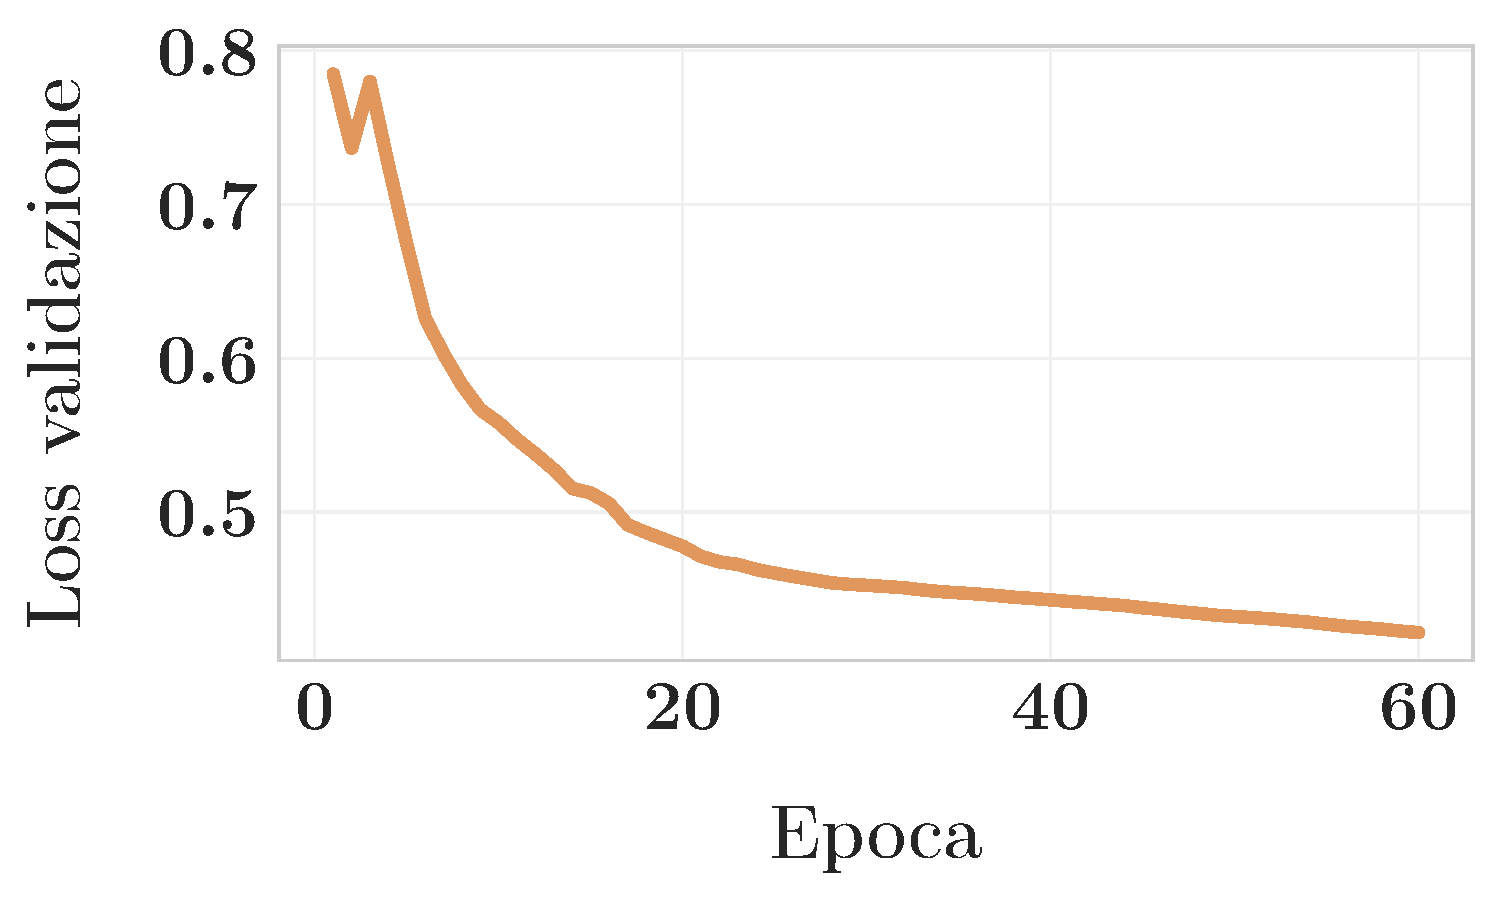
\includegraphics[width=0.48\textwidth]{images/domain-shift/sim-to-sim/1/validation-loss}}
	\hspace{0.01\textwidth}
	\\
	{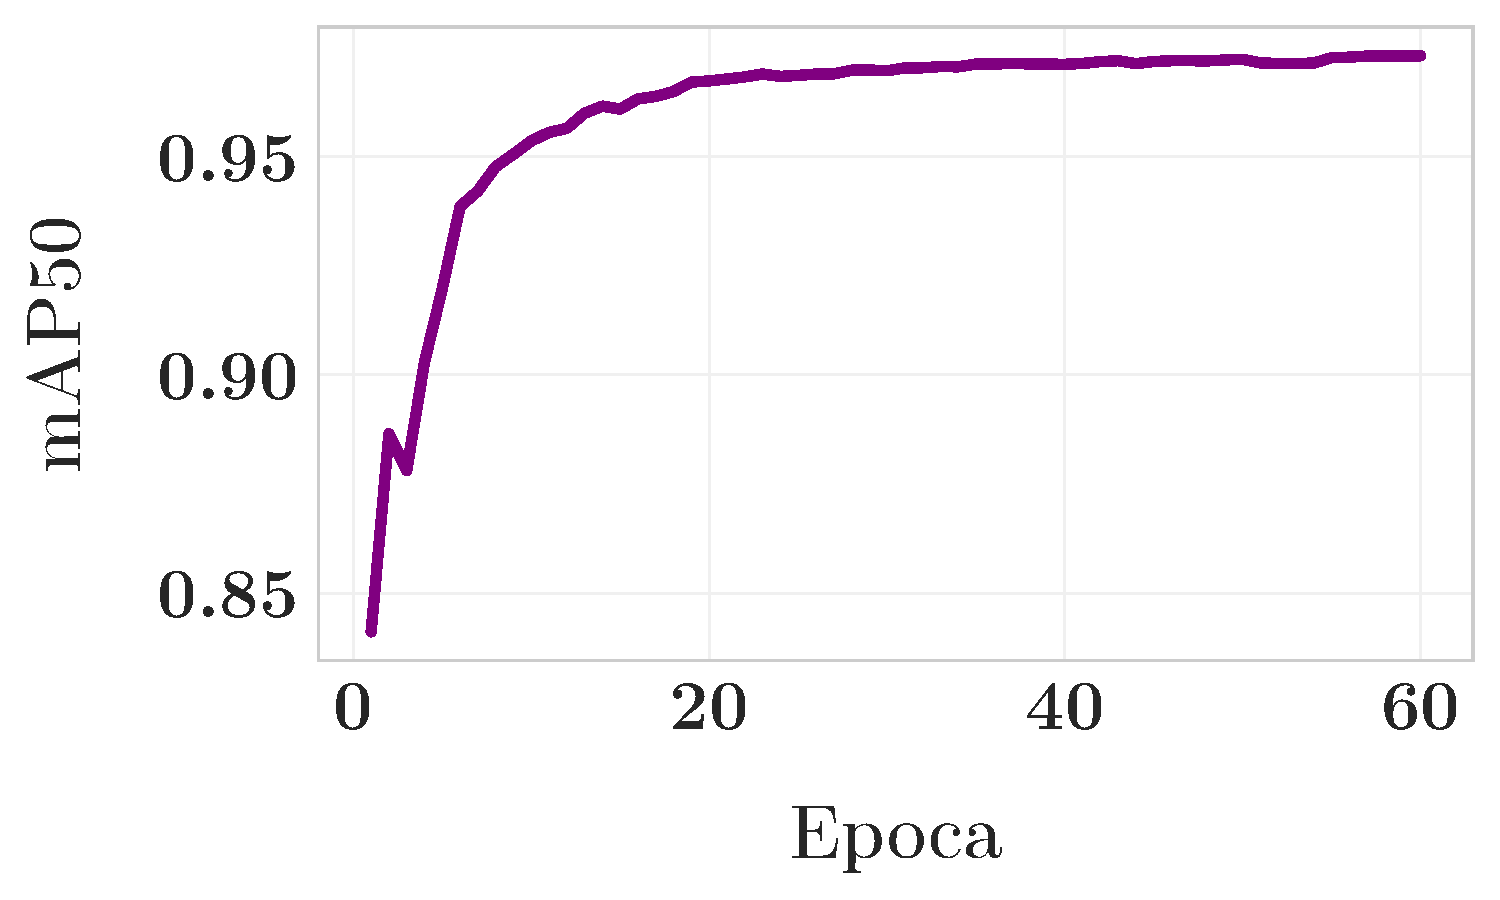
\includegraphics[width=0.48\textwidth]{images/domain-shift/sim-to-sim/1/map50}}
	\hspace{0.01\textwidth}
	{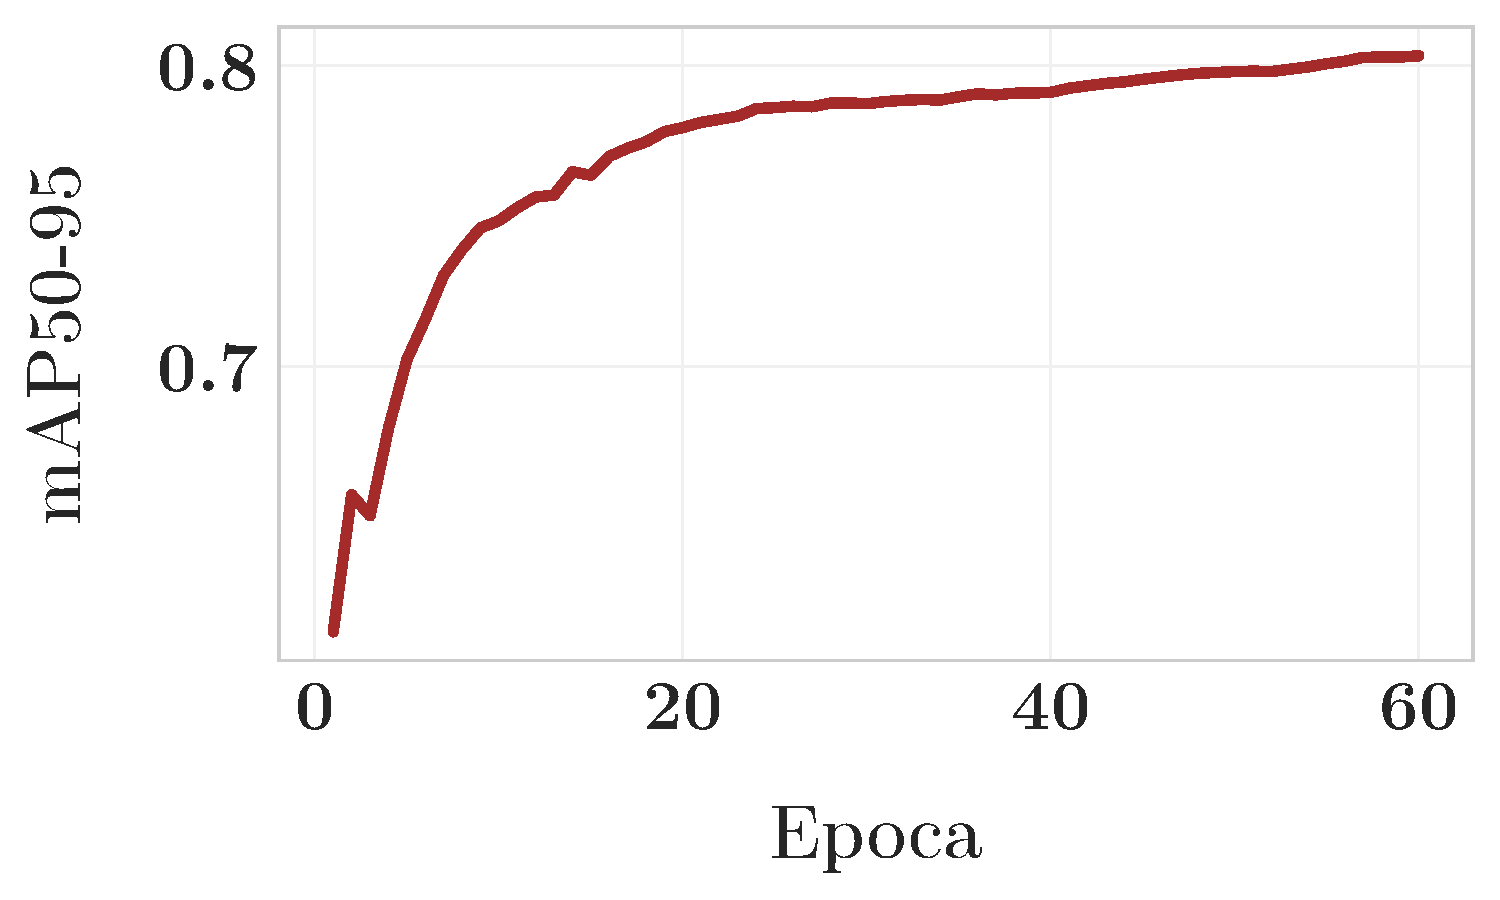
\includegraphics[width=0.48\textwidth]{images/domain-shift/sim-to-sim/1/map50-95}}
	\caption{Metriche di addestramento nel caso di ambienti simulati, con dati di validazione provenienti dagli stessi ambienti di training.}
	\label{fig:training-1}
\end{figure}

Si osserva come il modello performa quasi alla perfezione negli stessi ambienti di training. La mAP50 è infatti pari a 0.973, mentre la mAP50-95 raggiunge valori di 0.803. In genere un modello si può considerare utilizzabile se la sua mAP50 supera lo 0.4. L'analisi dei grafici delle loss mostra un decremento costante sia per i dati di training e di validazione, e questo permette di escludere fenomeni di overfitting o underfitting. L'andamento indica quindi un processo di ottimizzazione stabile ed efficace. Un esempio di dato originale e segmentato dal modello è mostrato nella \hyperref[fig:prediction-1]{Figura \ref{fig:prediction-1}}.

\begin{figure}[h!]
	\centering
	\subfloat[]{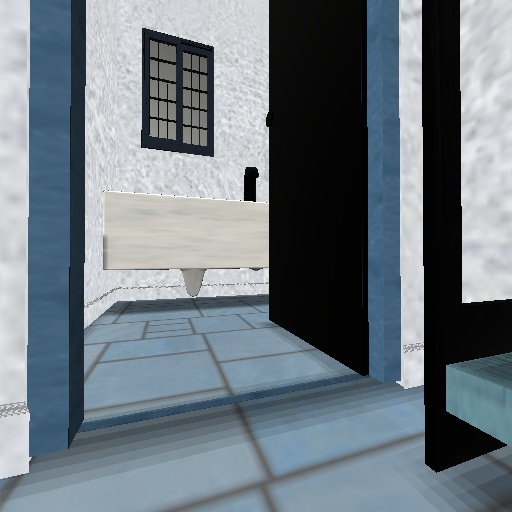
\includegraphics[width=0.42\textwidth]{images/domain-shift/sim-to-sim/1/original-1.jpg}}
	\hspace{0.01\textwidth}
	\subfloat[]{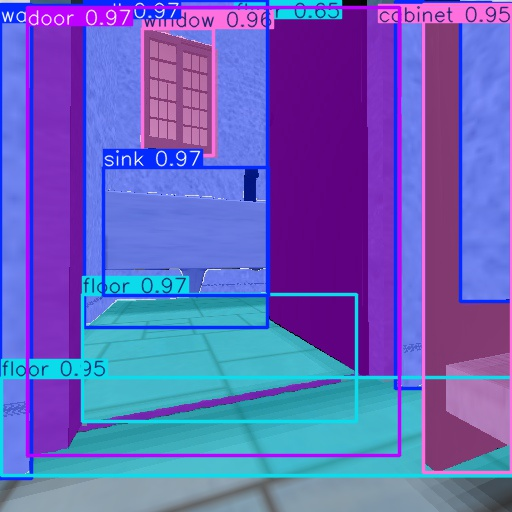
\includegraphics[width=0.42\textwidth]{images/domain-shift/sim-to-sim/1/prediction-1.jpg}}
	\caption{Output del modello (b) considerando dati provenienti dal simulatore (a).}
	\label{fig:prediction-1}
\end{figure}

\subsubsection{Esperimento 2}
\label{sec:esperimento_2}

Si è quindi passati ad analizzare un altro scenario di domain shift, nel quale il modello viene prima addestrato su un insieme di ambienti, e poi testato in altri ambienti mai visti prima. In questo caso sono stati mantenuti inalterati i dati di addestramento dell'esperimento precedente, mentre sono state utilizzate altre 4401 immagini provenienti da 3 diversi ambienti per il testing. Per questo esperimento, l'addestramento è stato svolto sul PC1, mantenendo tutti i restanti parametri inalterati. Le metriche di addestramento ottenute dopo 15 ore di training sono illustrate nella \hyperref[fig:training-2]{Figura \ref{fig:training-2}}.

\begin{figure}[h!]
	\centering
	{\includegraphics[width=0.48\textwidth]{images/domain-shift/sim-to-sim/2/train-loss}}
	\hspace{0.01\textwidth}
	{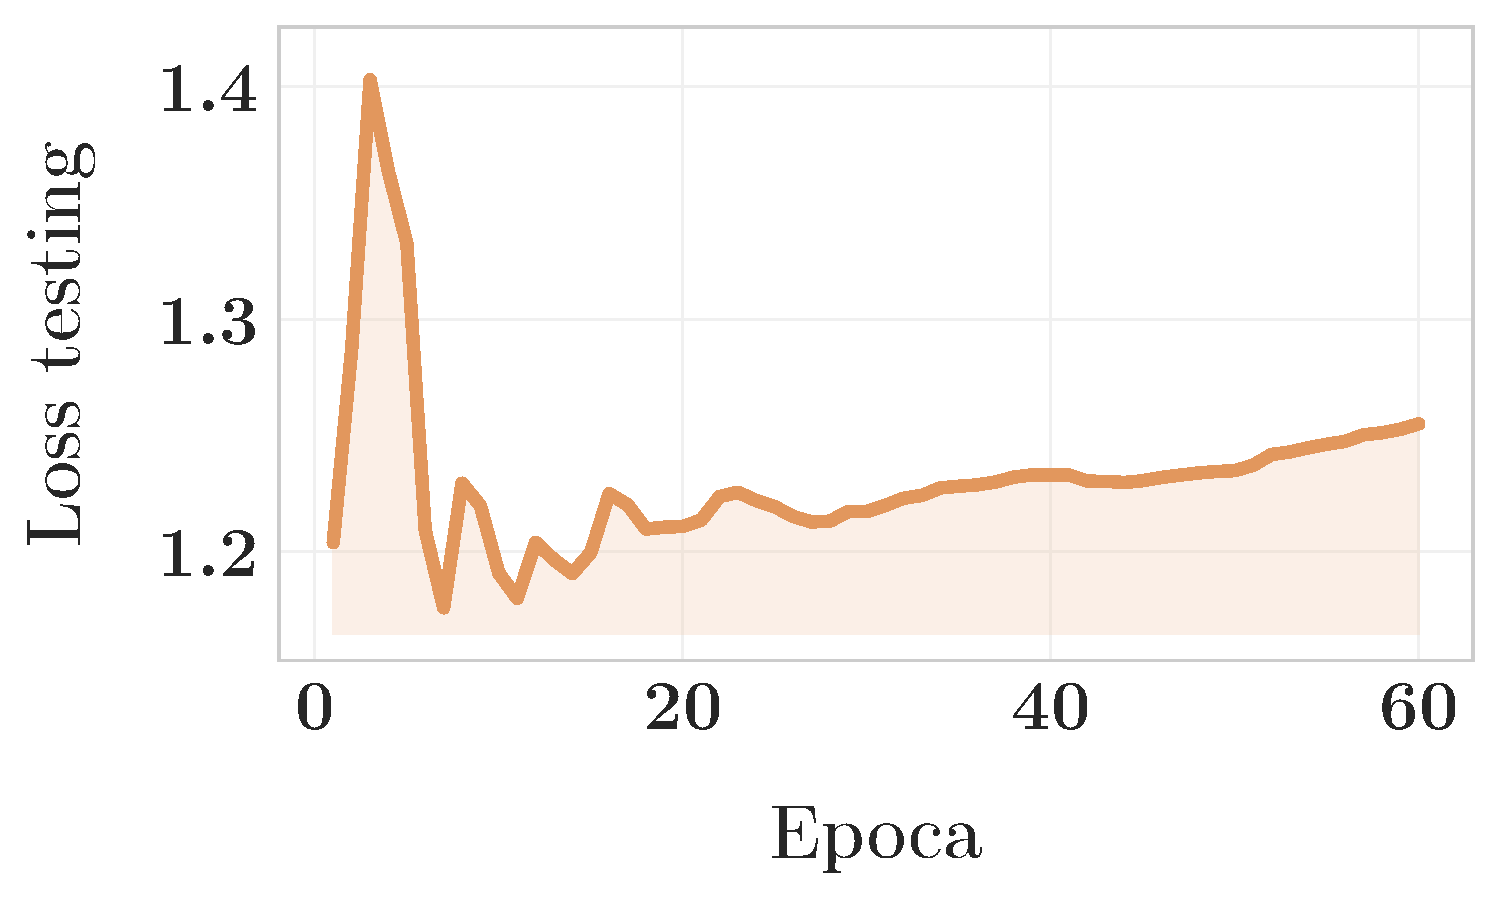
\includegraphics[width=0.48\textwidth]{images/domain-shift/sim-to-sim/2/testing-loss}}
	\hspace{0.01\textwidth}
	\\
	{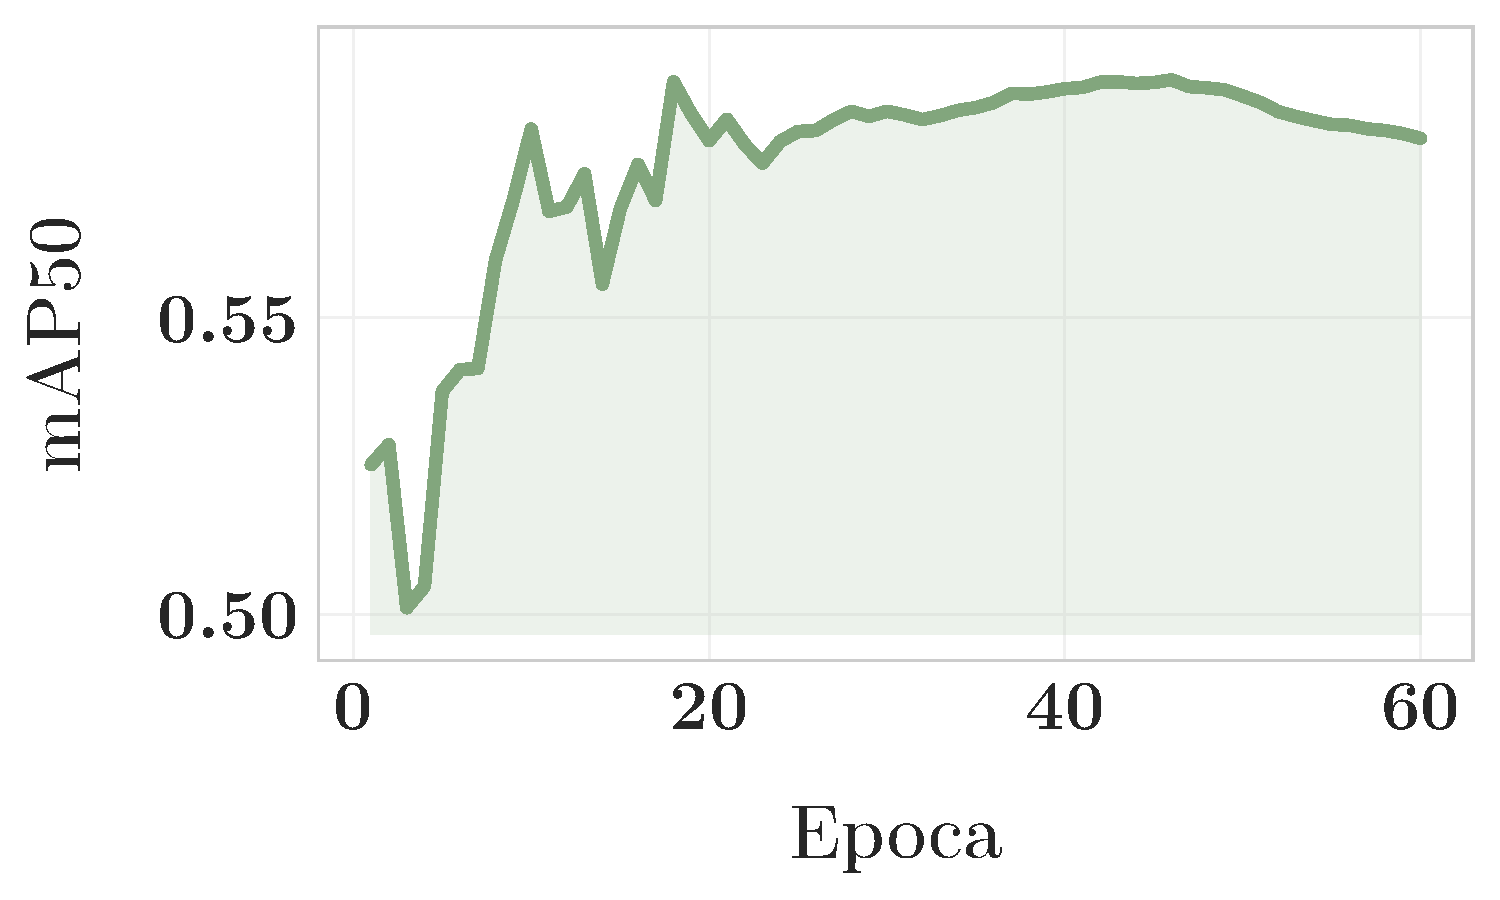
\includegraphics[width=0.48\textwidth]{images/domain-shift/sim-to-sim/2/map50}}
	\hspace{0.01\textwidth}
	{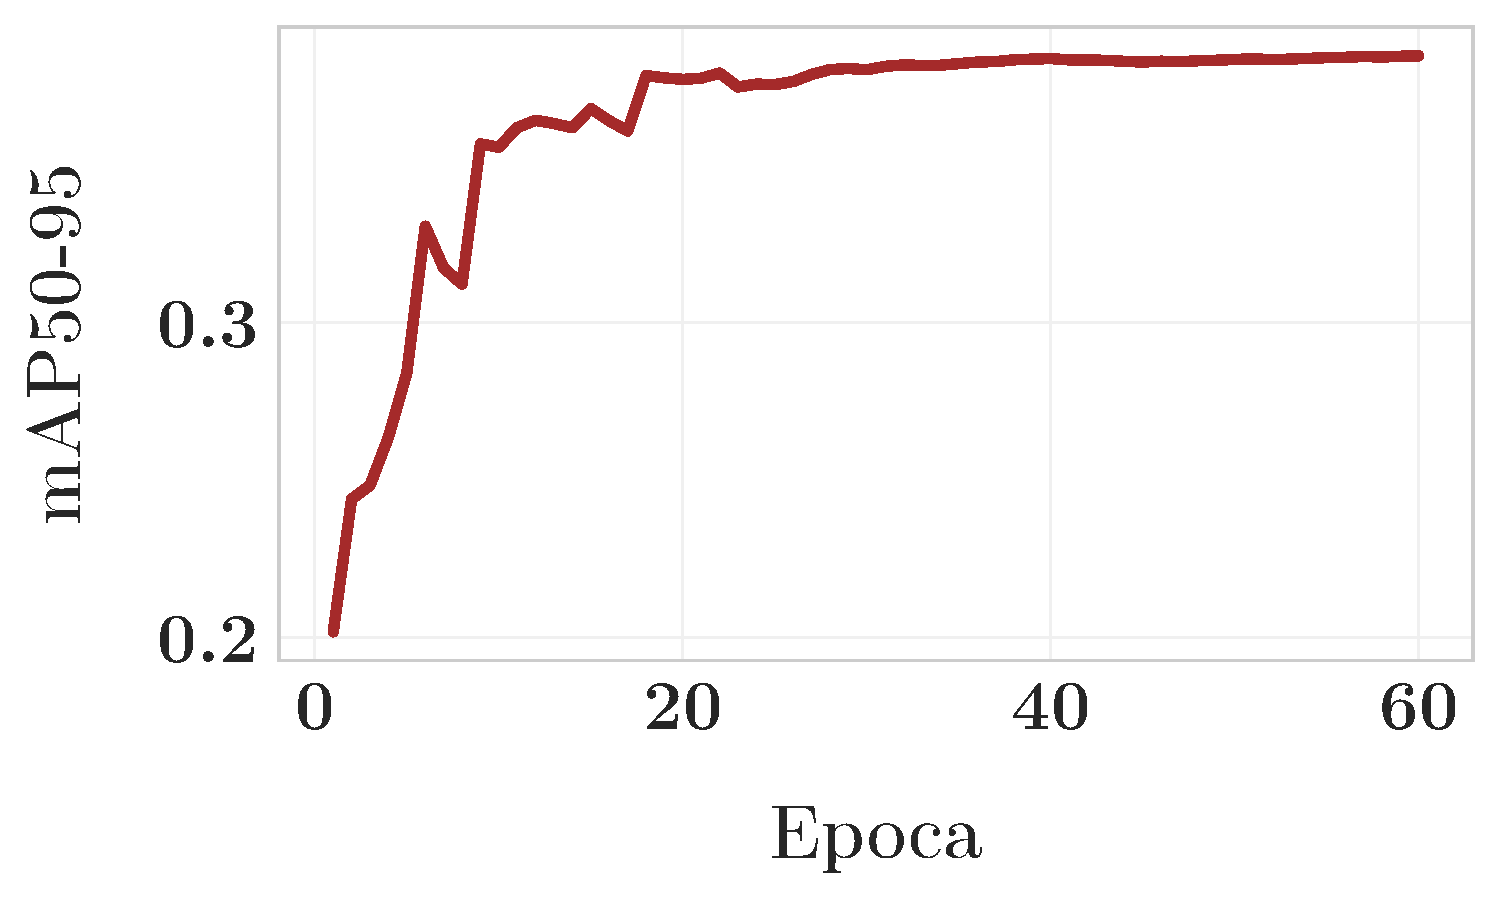
\includegraphics[width=0.48\textwidth]{images/domain-shift/sim-to-sim/2/map50-95}}
	\caption{Metriche di addestramento nel caso di ambienti simulati, con dati di testing diversi da quelli utilizzati per il training.}
	\label{fig:training-2}
\end{figure}

I risultati mostrano un impatto significativo dovuto al domain shift sulle prestazioni del modello. Le immagini di testing contengono infatti oggetti, texture e planimetrie differenti dispetto a quelle utilizzate per il training, il che rende la generalizzazione più complessa. In aggiunta, nelle scene di testing, oggetti appartenenti ad una stessa classe possono presentare forme e colori diversi rispetto a quelli visti in addestramento.

Di conseguenza, la mAP50 finale è pari a 0.580 mentre la mAP50-95 risulta essere 0.432. Si ha quindi un calo di prestazioni rispettivamente di 0.393 e 0.371 rispetto all'\hyperref[sec:esperimento_1]{Esperimento 1}. Questo calo è significativo e conferma l'impatto del domain shift, ma potrebbe essere mitigato aumentando la varietà degli ambienti di addestramento.

Inoltre è interessante notare come le metriche di mAP raggiungano il loro picco massimo all'epoca 47, per poi deteriorarsi in maniera progressiva. Questo indica che proseguire l'addestramento oltre questa soglia non migliorerebbe le prestazioni, ma anzi le peggiorerebbe.  In questo caso, aumentare il numero di epoche di addestramento non farebbe altro che diminuire la mAP. Per ottimizzare tempo, risorse e ottenere il miglior modello possibile, l'addestramento dovrebbe essere interrotto all'epoca 47.

\subsubsection{Esperimento 3}
\label{sec:esperimento_3}

Per concludere, è stato anche creato un terzo modello utilizzato in esperimenti successivi. In questo caso si è addestrato YOLO11 con 35000 immagini provenienti da tutti e 15 gli ambienti, e ottenute nel corso di 30 diverse run. Per la validazione sono state invece utilizzate 5000 immagini provenienti dagli stessi 15 ambienti. Il modello è stato addestrato sul PC1 per 15 ore e per un totale di 60 epoche, e le metriche ottenute risultano molto simili al quelle del primo esperimento. L'unica differenza riguarda la mAP50 e mAP50-95 in qunato leggermente più basse, rispettivamente a 0.966 e 0.784. Questo può essere dovuto alla maggior variabilità introdotta dalle immagini provenienti da più ambienti, rendendo necessario un numero maggiore di epoche per ottenere gli stessi valori.

\subsection{Real-to-real}
\label{sec:real_to_real}

Il secondo caso di studio riguarda l'analisi del domain shift in ambienti reali. Vengono addestrati modelli utilizzando 10, 50 e 395 diverse scene provenienti dal dataset ScanNet. Nel primo caso vengono mostrate le metriche di addestramento con informazioni relative alla validazione, mentre negli ultimi due casi vengono mostrate solo le più interessanti metriche di training con le loss di testing.

\subsubsection{Esperimento 4}
\label{sec:esperimento_4}

Per il primo esperimento sono state utilizzate 8956 immagini di training provenienti da 10 scene, e 1580 immagini per la validazione provenienti dagli stessi 10 ambienti. Il modello è stato addestrato per 60 epoche sul PC1, con batch di dimensione 12, risoluzione delle immagini a 640 pixel, e parametro \textit{rect} impostato a \textit{True}. Essendo le immagini di scannet rettangolari, con quest'ultima impostazione si evita di tagliare le immagini in un formato quadrato, e si indica la dimensione in pixel del lato più lungo, ovvero 640. Dopo 4 ore e 30 minuti di addestramento, sono state generate le metriche riportate nella \hyperref[fig:training-3]{Figura \ref{fig:training-3}}.

\begin{figure}[t]
	\centering
	{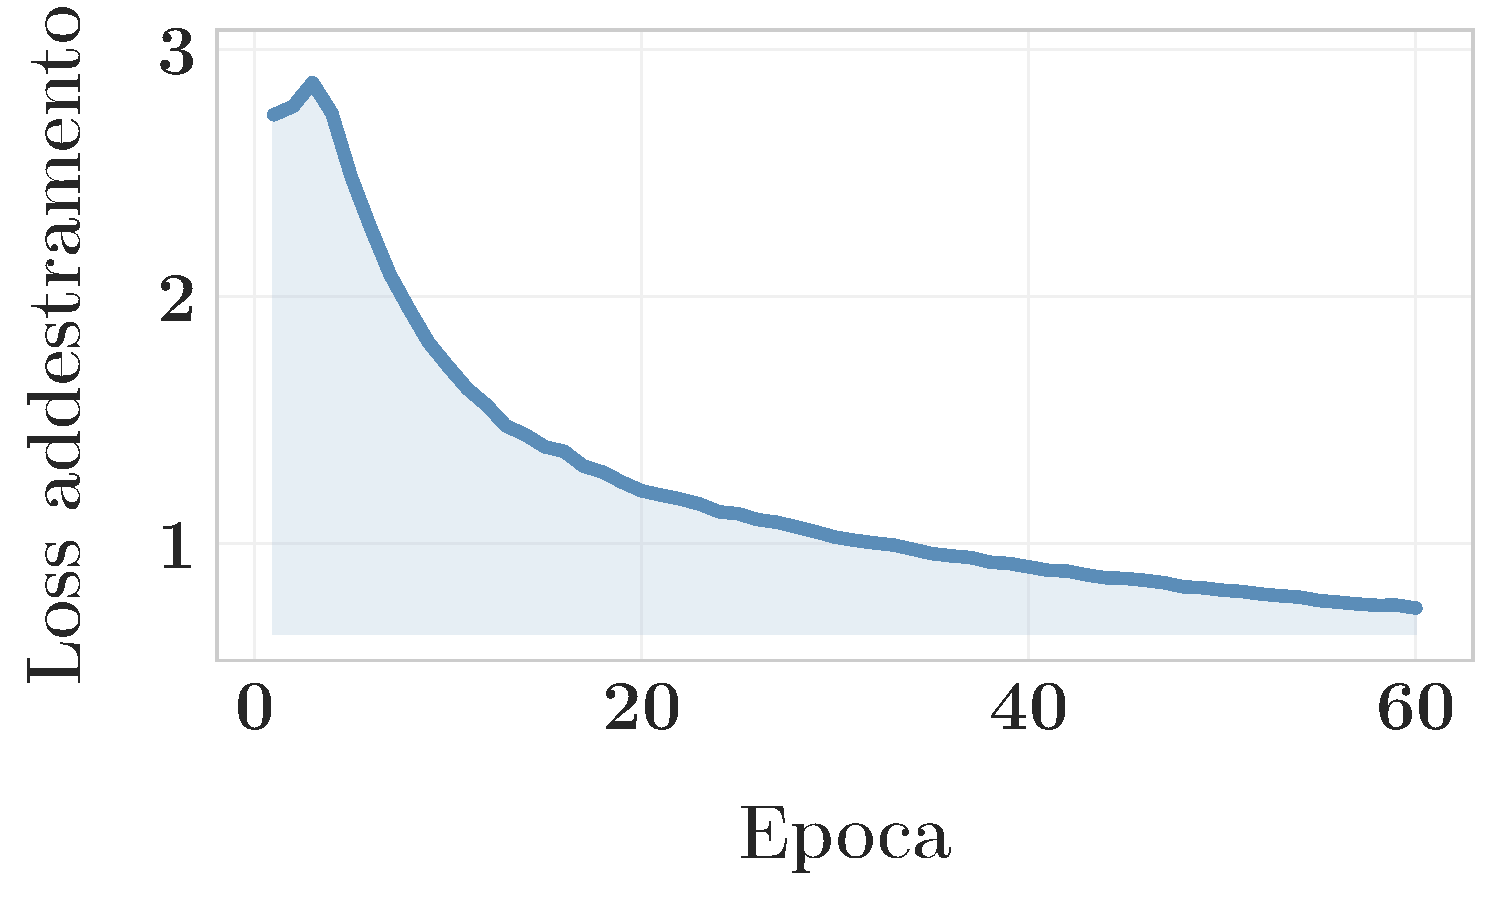
\includegraphics[width=0.48\textwidth]{images/domain-shift/real-to-real/4/train-loss}}
	\hspace{0.01\textwidth}
	{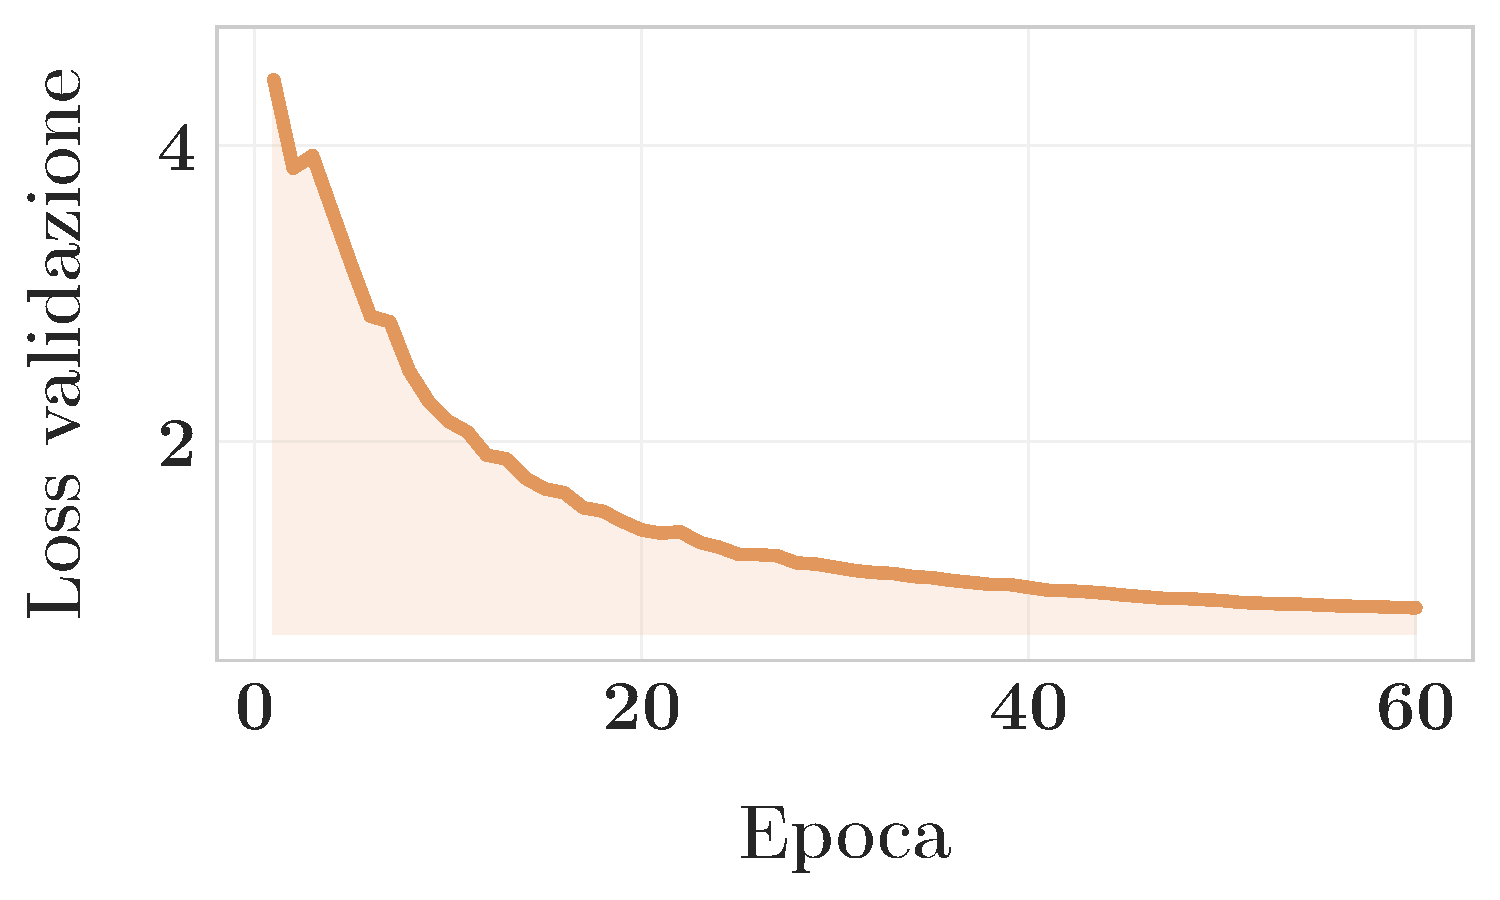
\includegraphics[width=0.48\textwidth]{images/domain-shift/real-to-real/4/validation-loss}}
	\hspace{0.01\textwidth}
	\\
	{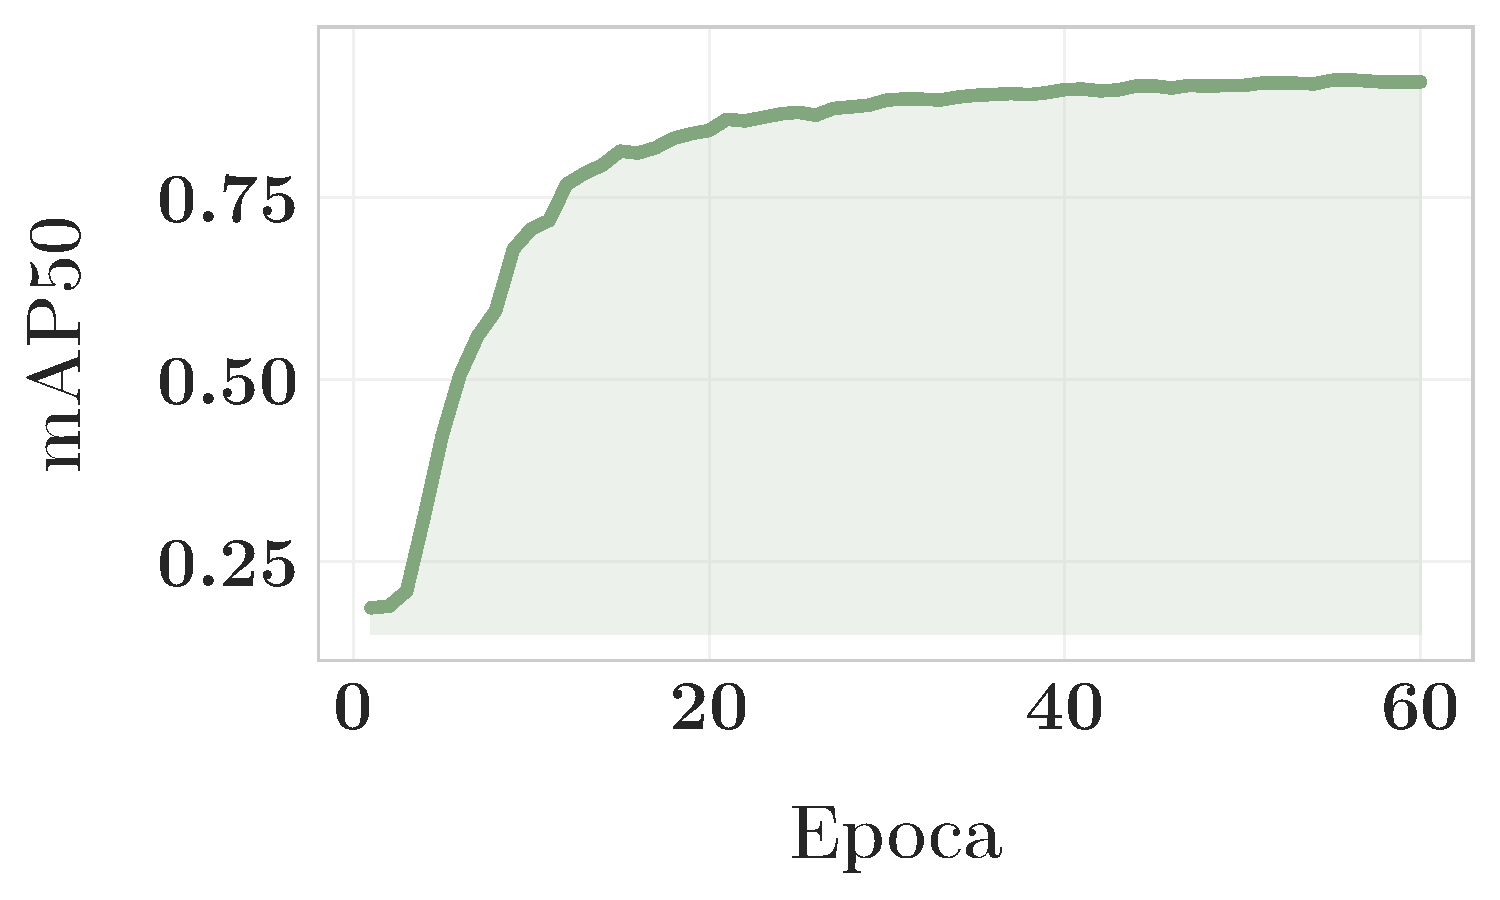
\includegraphics[width=0.48\textwidth]{images/domain-shift/real-to-real/4/map50}}
	\hspace{0.01\textwidth}
	{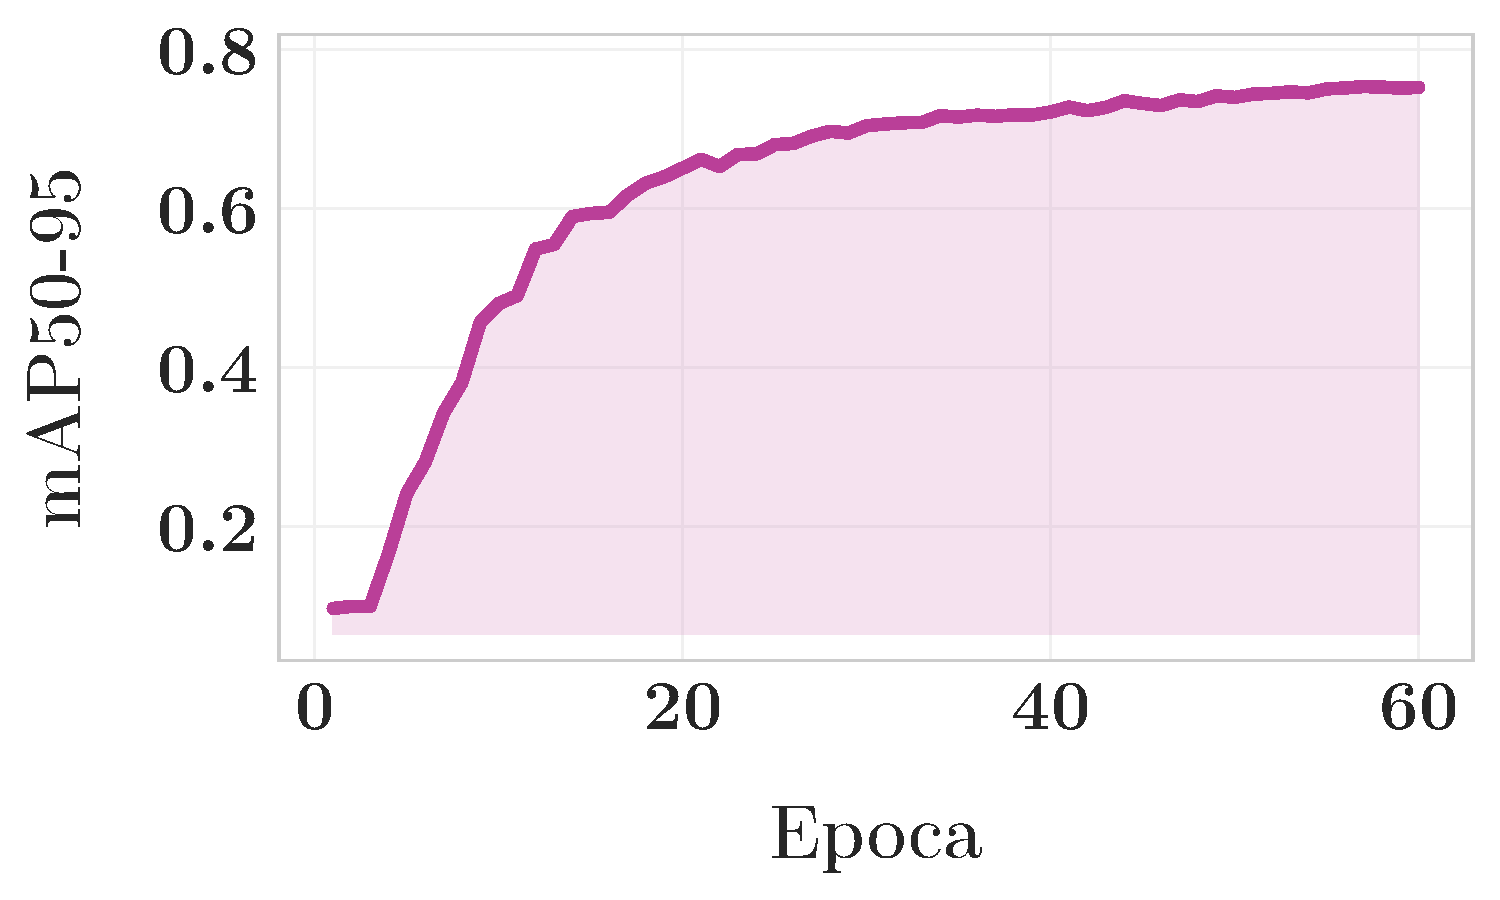
\includegraphics[width=0.48\textwidth]{images/domain-shift/real-to-real/4/map50-95}}
	\caption{Metriche di addestramento nel caso di 10 ambienti reali, con dati di validazione provenienti dagli stessi ambienti di training.}
	\label{fig:training-3}
\end{figure}

Come quanto visto nella sezione sim-to-sim, anche qui il modello apprende quasi alla perfezione negli stessi ambienti di training. In particolare la mAP50 e la mAP50-95 sono rispettivamente 0.908 e 0.753, valori leggermente più bassi del caso sim-to-sim, ma comunque ottimi. Questa differenza è principalmente dovuta alla maggior complessità delle scene reali, che presentano un dettaglio e variabilità maggiore rispetto a quelle simulate. Anche in questo esperimento l'andamento delle loss indica che il modello non presenta overfitting o underfitting. La \hyperref[fig:prediction-2]{Figura \ref{fig:prediction-2}} mostra un esempio di dato originale e la relativa segmentazione ottenuta da questo modello.

\begin{figure}[h!]
	\centering
	\subfloat[]{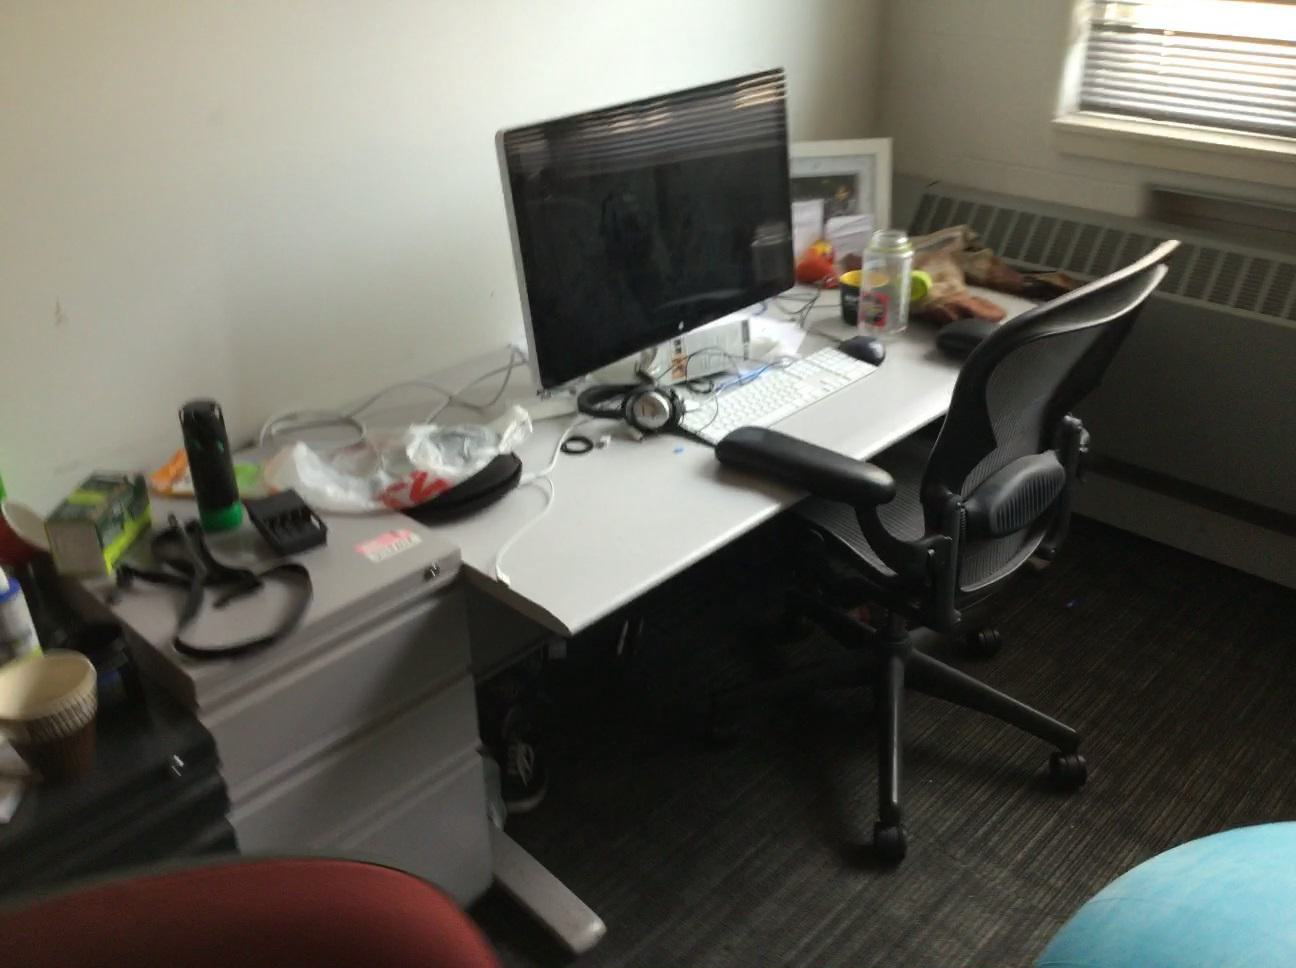
\includegraphics[width=0.42\textwidth]{images/domain-shift/real-to-real/4/original-1.jpg}}
	\hspace{0.01\textwidth}
	\subfloat[]{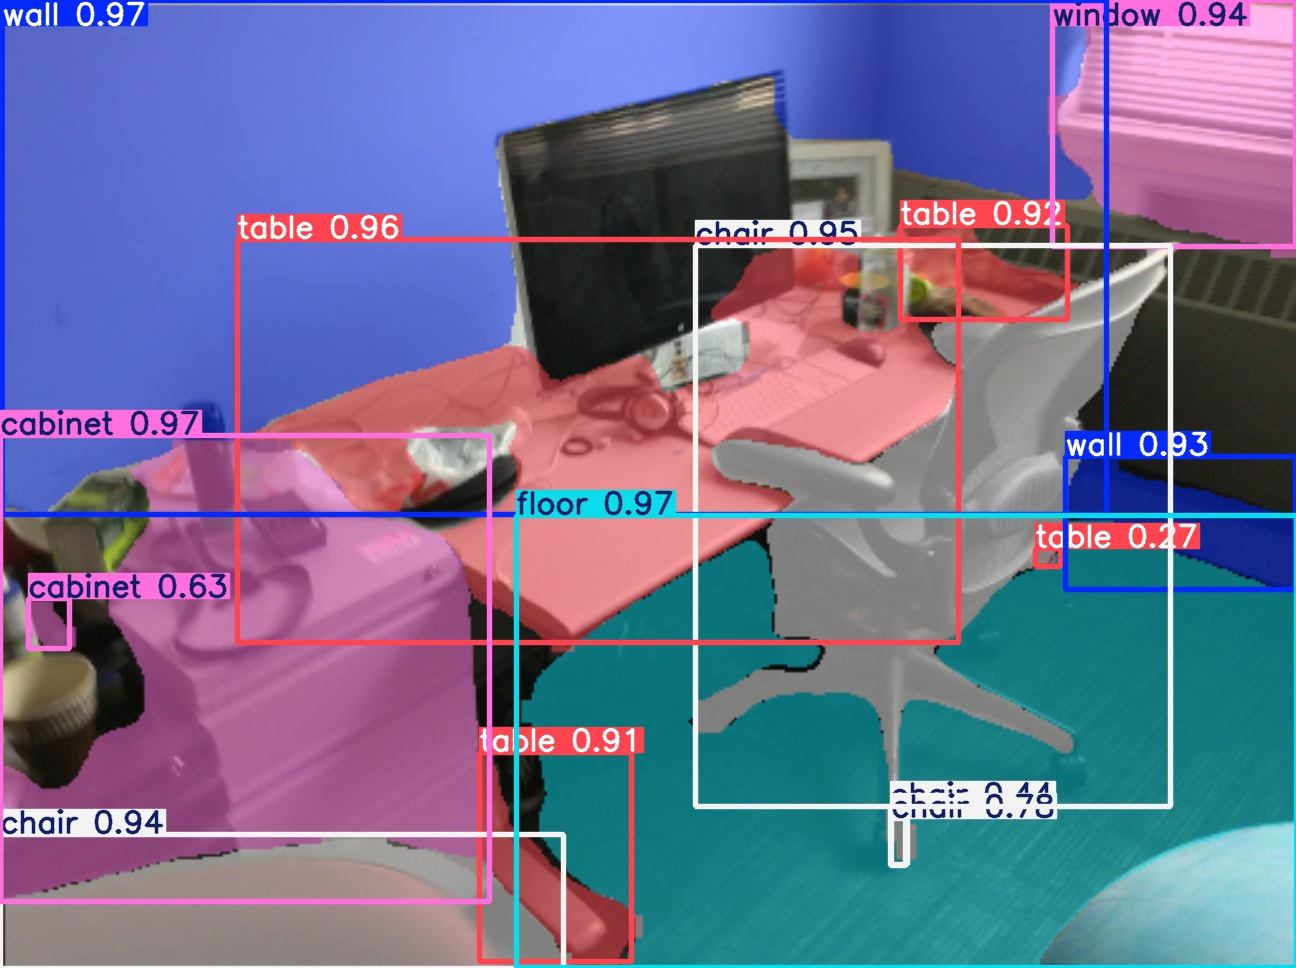
\includegraphics[width=0.42\textwidth]{images/domain-shift/real-to-real/4/prediction-1.jpg}}
	\caption{Output del modello (b) considerando un'immagine presa dalle 10 scene ScanNet usate per l'addestramento (a).}
	\label{fig:prediction-2}
\end{figure}

A causa del basso numero di scene utilizzate per addestrare questo modello, ha poco senso analizzare le performance in testing. Di contro, nei prossimi esperimenti non verrà più mostrato l'andamento di training e validazione, in quanto praticamente identico a tutti i casi già visti fino ad ora. Saranno invece mostrate le metriche di training con dati di testing.

\subsubsection{Esperimento 5}
\label{sec:esperimento_5}

Nel seguente espetimento è stato addestrato il modello YOLO11 con 8000 immagini provenienti da 50 diverse scene. Successivamente è stato validato con 1000 immagini provenienti dagli stessi 50 ambienti, e testato con altre 1000 immagini provenienti da 20 ambienti non utilizzati per il training. Il modello è stato poi addestrato per 60 epoche con batch size di 10 sul PC1, per una durata totale di 4 ore. Le metriche di training e testing sono riportate in \hyperref[fig:training-4]{Figura \ref{fig:training-4}}.

\begin{figure}[h!]
	\centering
	{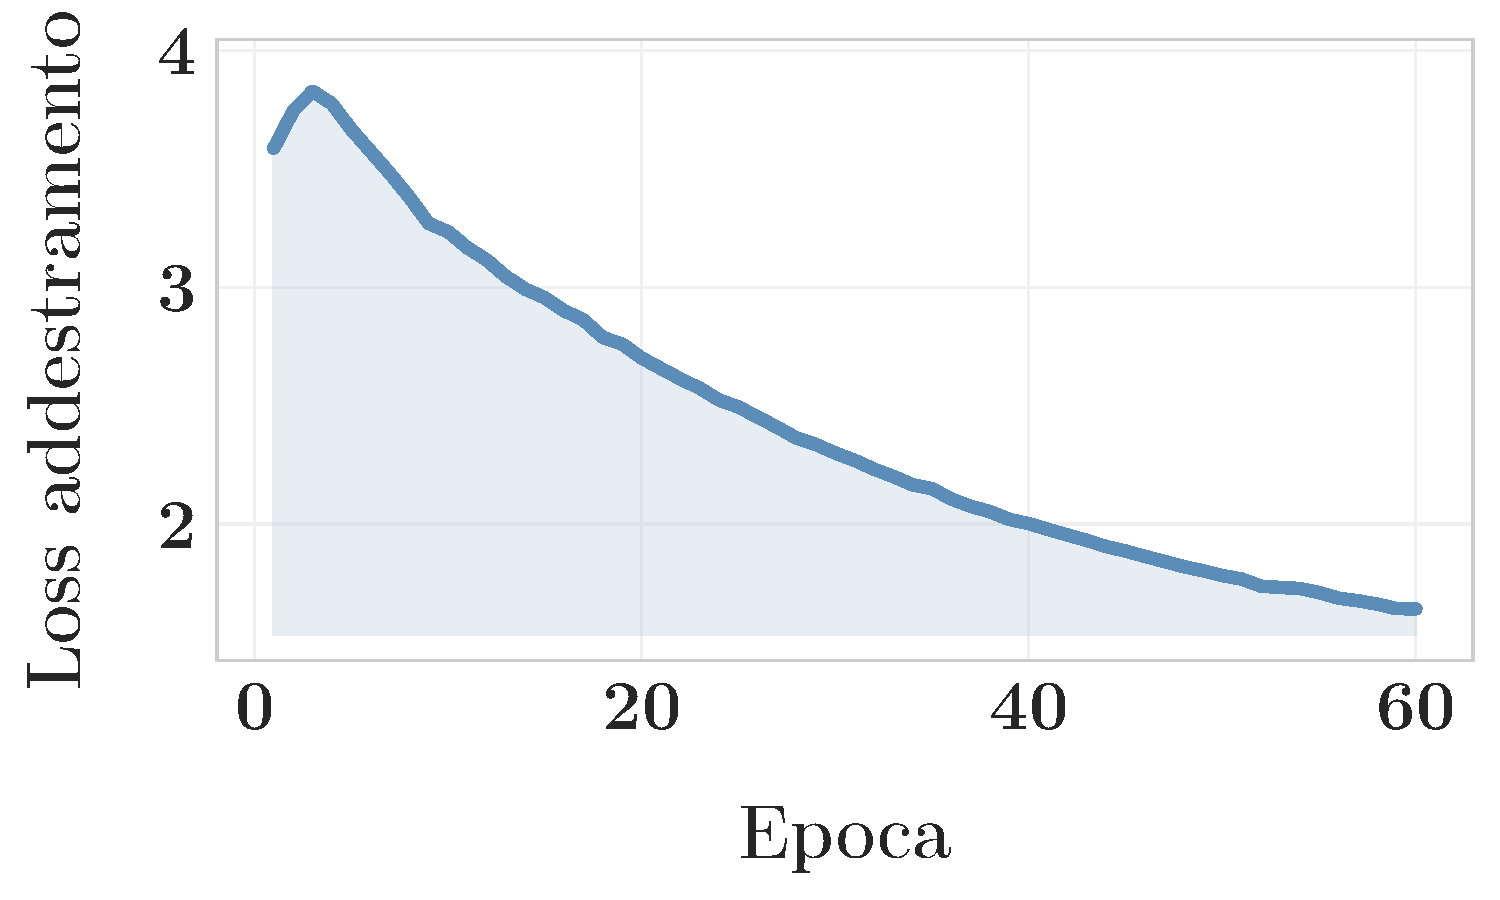
\includegraphics[width=0.48\textwidth]{images/domain-shift/real-to-real/5/train-loss}}
	\hspace{0.01\textwidth}
	{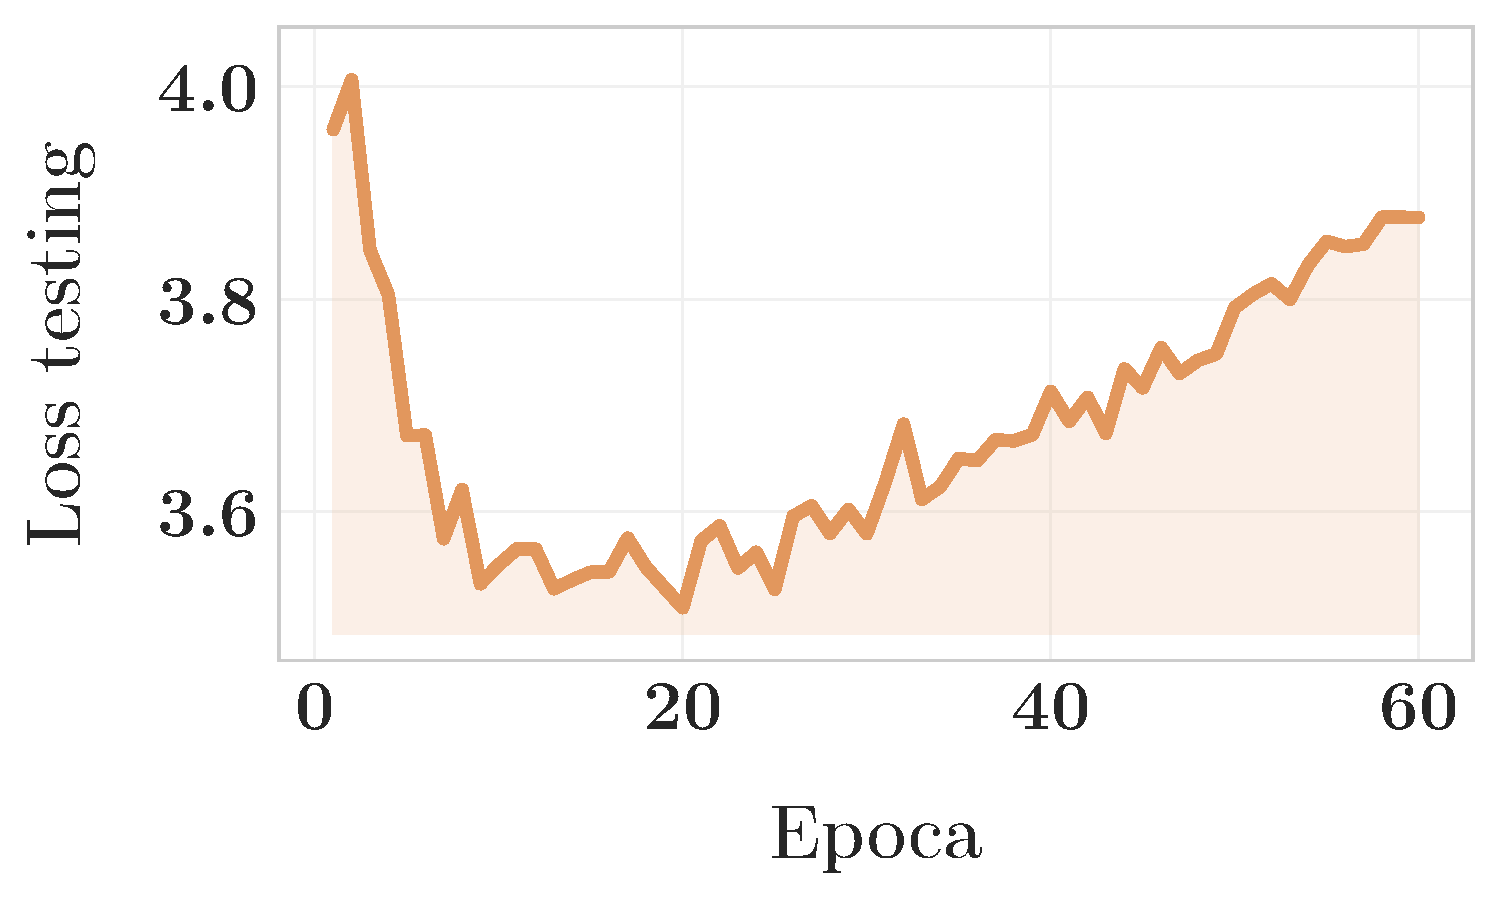
\includegraphics[width=0.48\textwidth]{images/domain-shift/real-to-real/5/testing-loss}}
	\hspace{0.01\textwidth}
	\\
	{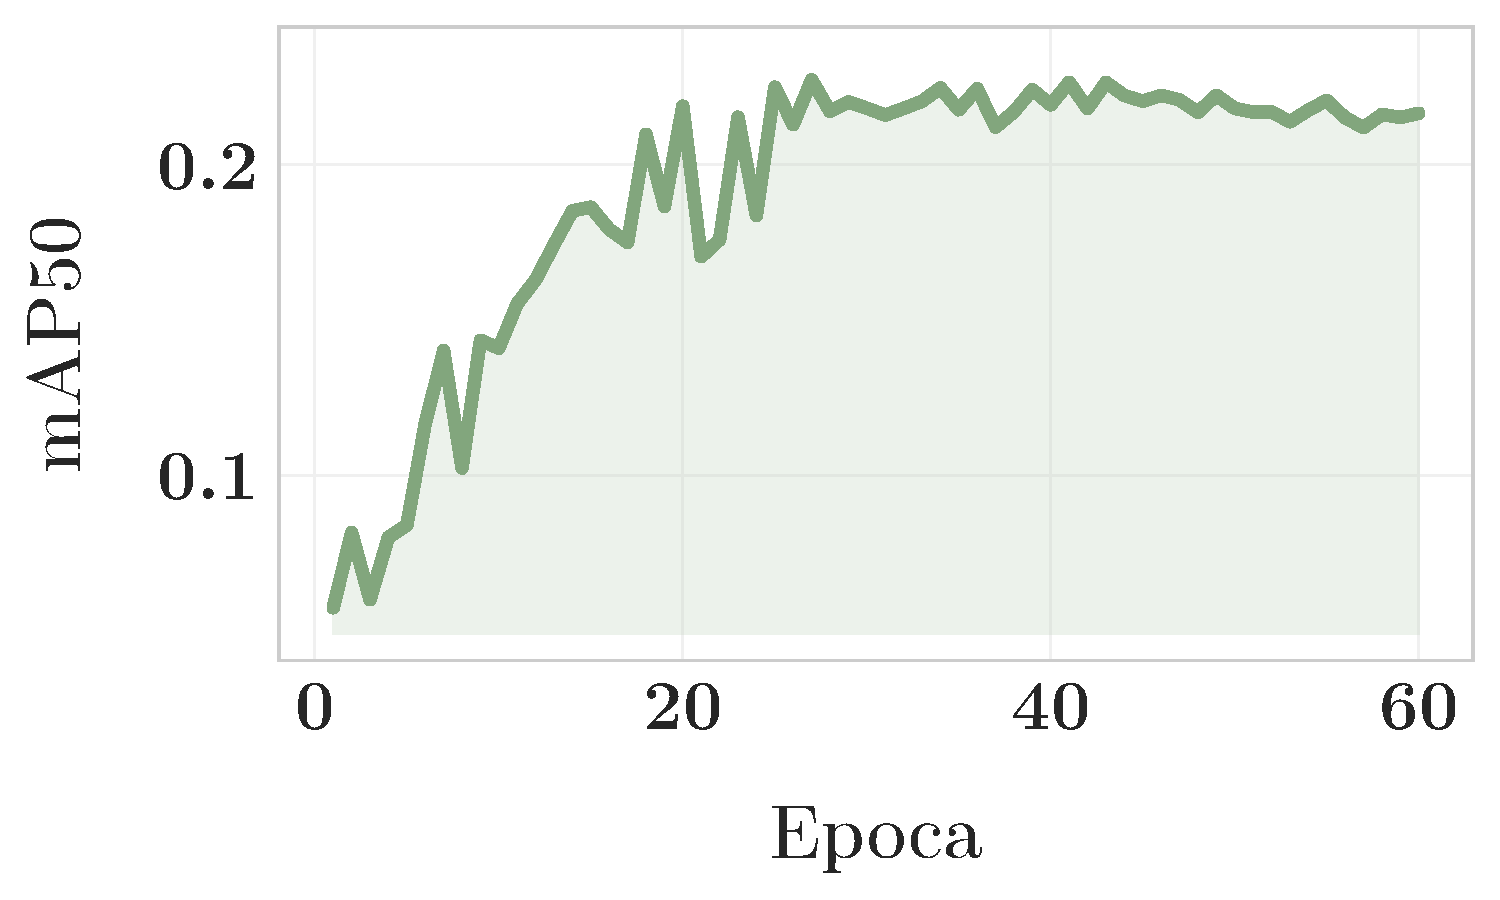
\includegraphics[width=0.48\textwidth]{images/domain-shift/real-to-real/5/map50}}
	\hspace{0.01\textwidth}
	{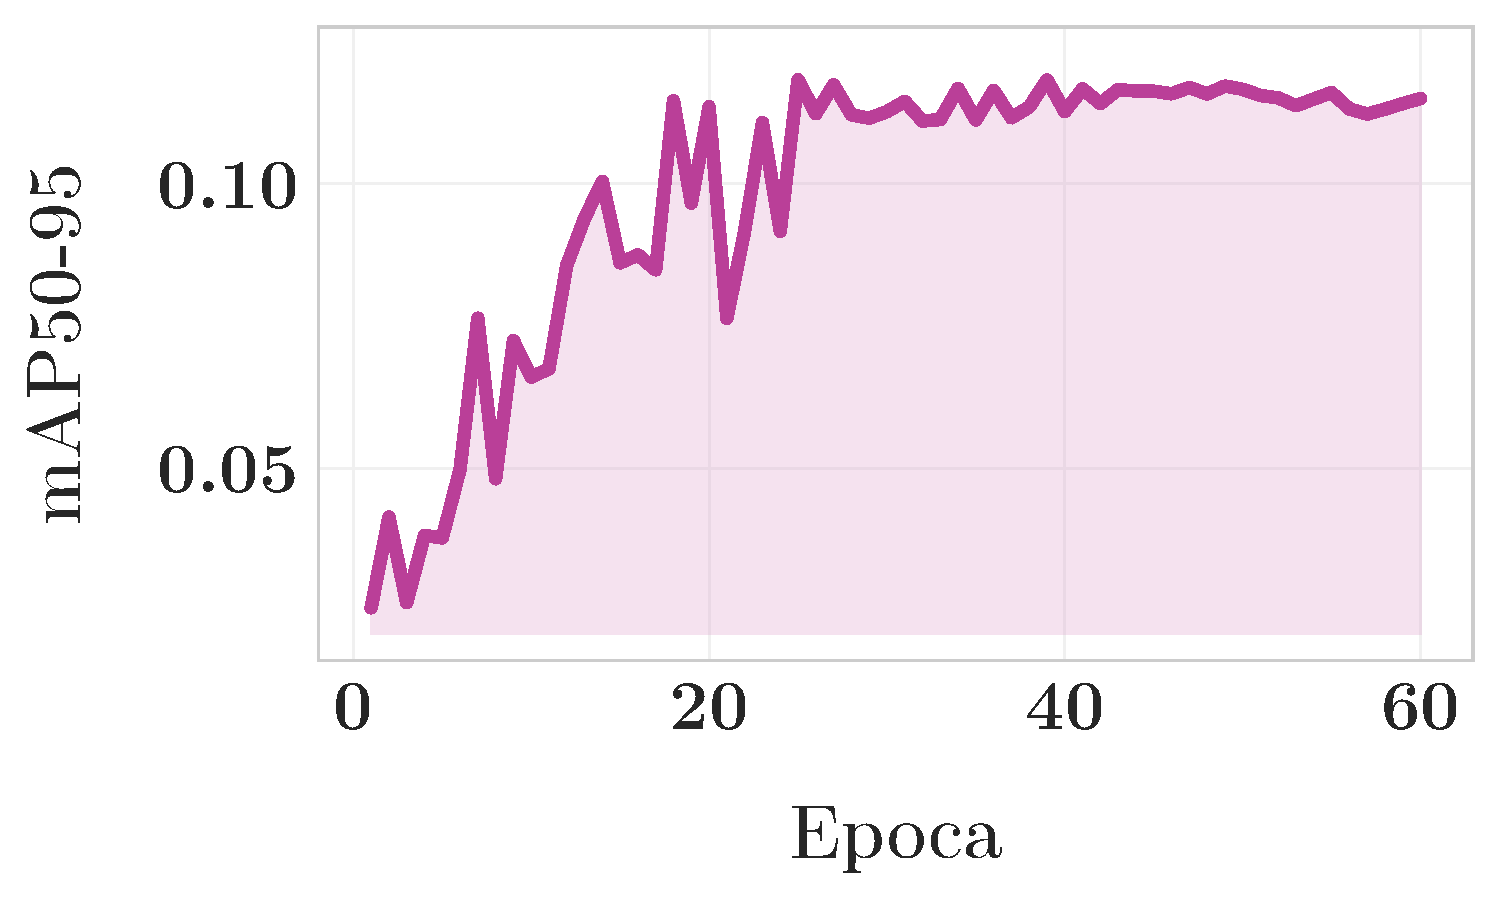
\includegraphics[width=0.48\textwidth]{images/domain-shift/real-to-real/5/map50-95}}
	\caption{Metriche di addestramento nel caso di 50 ambienti reali, con dati di testing provenienti da 20 diversi ambienti.}
	\label{fig:training-4}
\end{figure}

Osservando i grafici della loss di addestramento e testing, si nota che con l'avanzare delle epoche il modello migliora le proprie capacità di segmentare oggetti. Nonostante questo, la loss di testing ci dice che a partire dall'epoca 30, il modello inizia ad avere i primi segnali di overfitting, ma non sembra avere un impatto negativo sull'andamento delle curve di mAP. Dai grafici delle mAP si deduce invece che il modello impara a segmentare correttamente gli oggetti. La mAP50 al suo picco (epoca 27) risulta essere 0.227, mentre la mAP50-95 alla stessa epoca misura 0.117.

A confronto i dati di validazione presi dalle stesse immagini di addestramento mostrano una mAP50 di 0.636 e una mAP50-95 di 0.415. Anche in questo caso si nota un domain shift abbastanza marcato, simile a quanto già visto nell'\hyperref[sec:esperimento_2]{Esperimento 2} della sezione sim-to-sim. Questo può essere principalmente causato dal basso numero di ambienti utilizzati, che non riescono a catturare adeguatamente la diversità presente nei dati di testing.

\subsubsection{Esperimento 6}
\label{sec:esperimento_6}

Per verificare l'ultima ipotesi formulata, in questo esperimento è stato utilizzato un dataset più grande, composto da 8000 immagini provenienti da 395 scene diverse. Le immagini di testing sono rimaste invariate rispetto all'esperimento precedente, mentre quelle di validazione sono sempre 1000 e provengono dagli stessi ambienti di training. Anche i parametri utilizzati per l'addestramento sono rimasti invariati. I risultati del training sono illustrati nella \hyperref[fig:training-5]{Figura \ref{fig:training-5}}.

\begin{figure}[h!]
	\centering
	{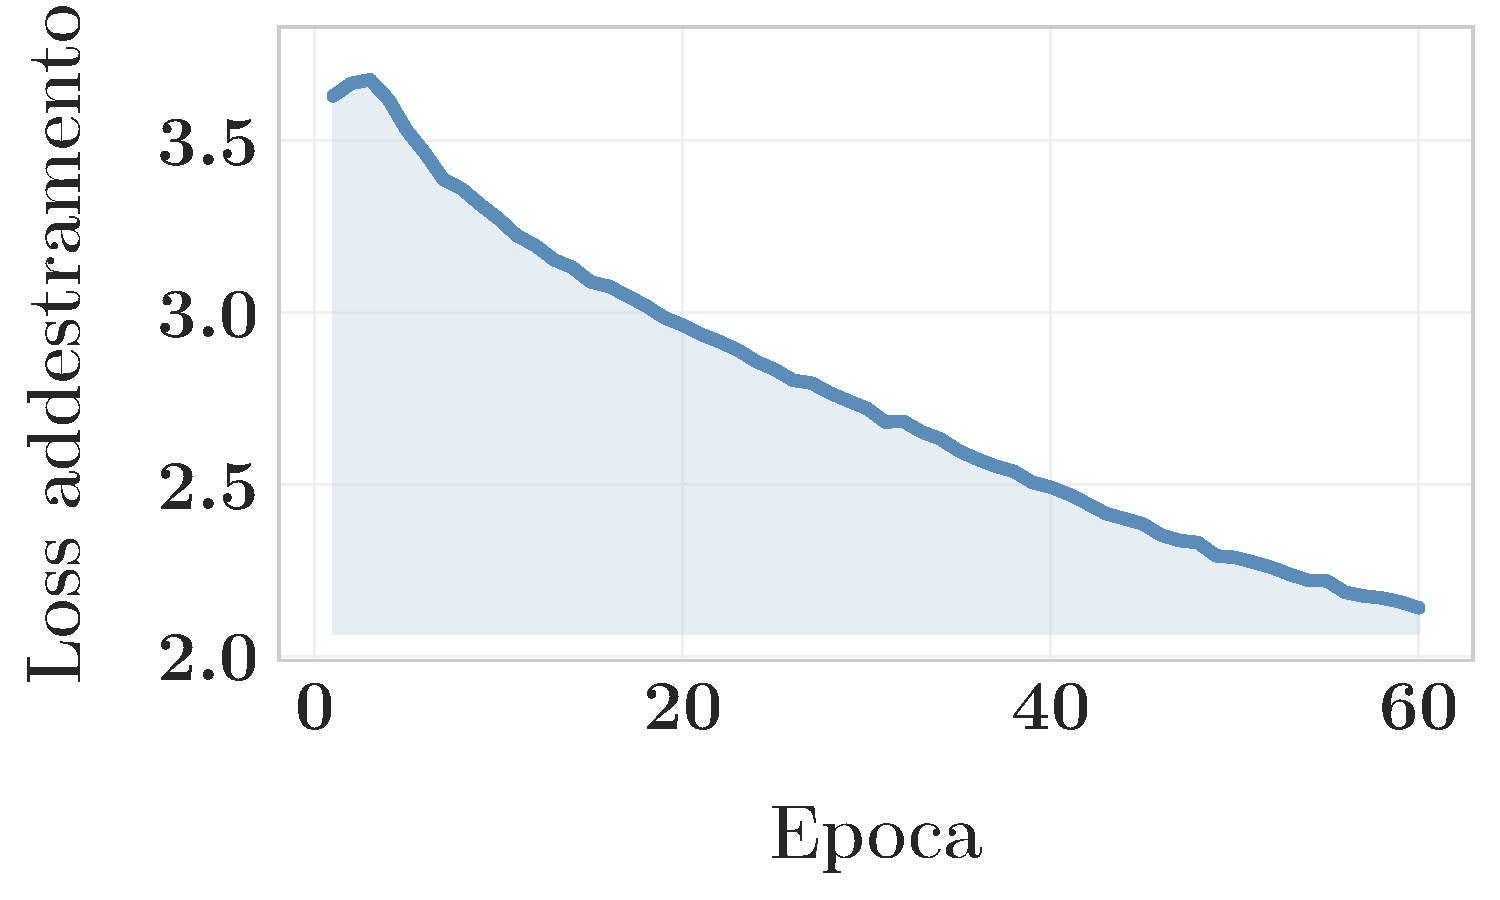
\includegraphics[width=0.48\textwidth]{images/domain-shift/real-to-real/6/train-loss}}
	\hspace{0.01\textwidth}
	{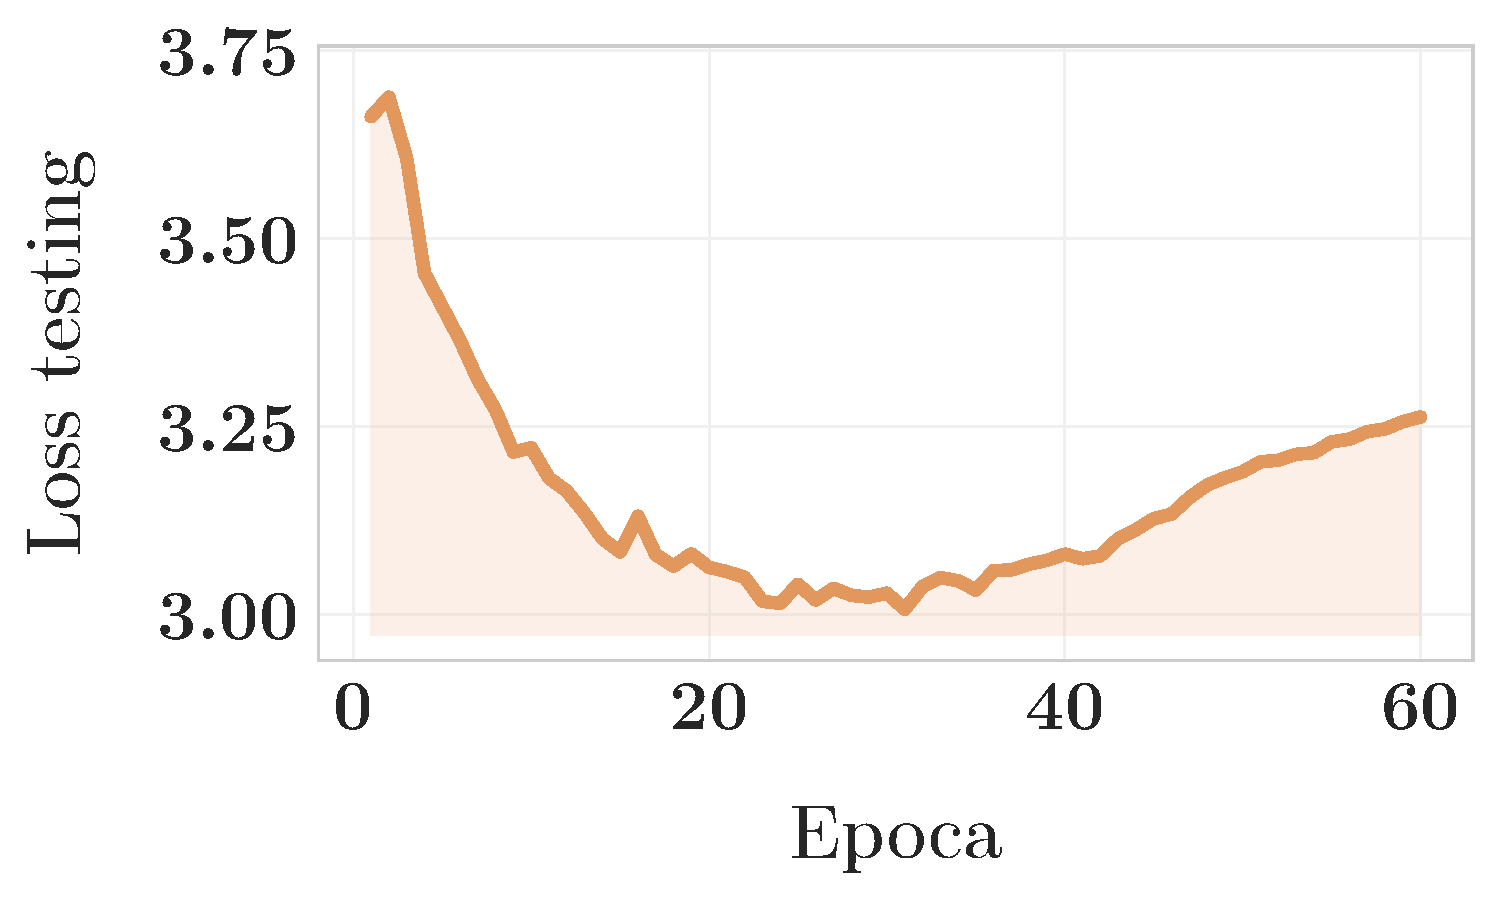
\includegraphics[width=0.48\textwidth]{images/domain-shift/real-to-real/6/testing-loss}}
	\hspace{0.01\textwidth}
	\\
	{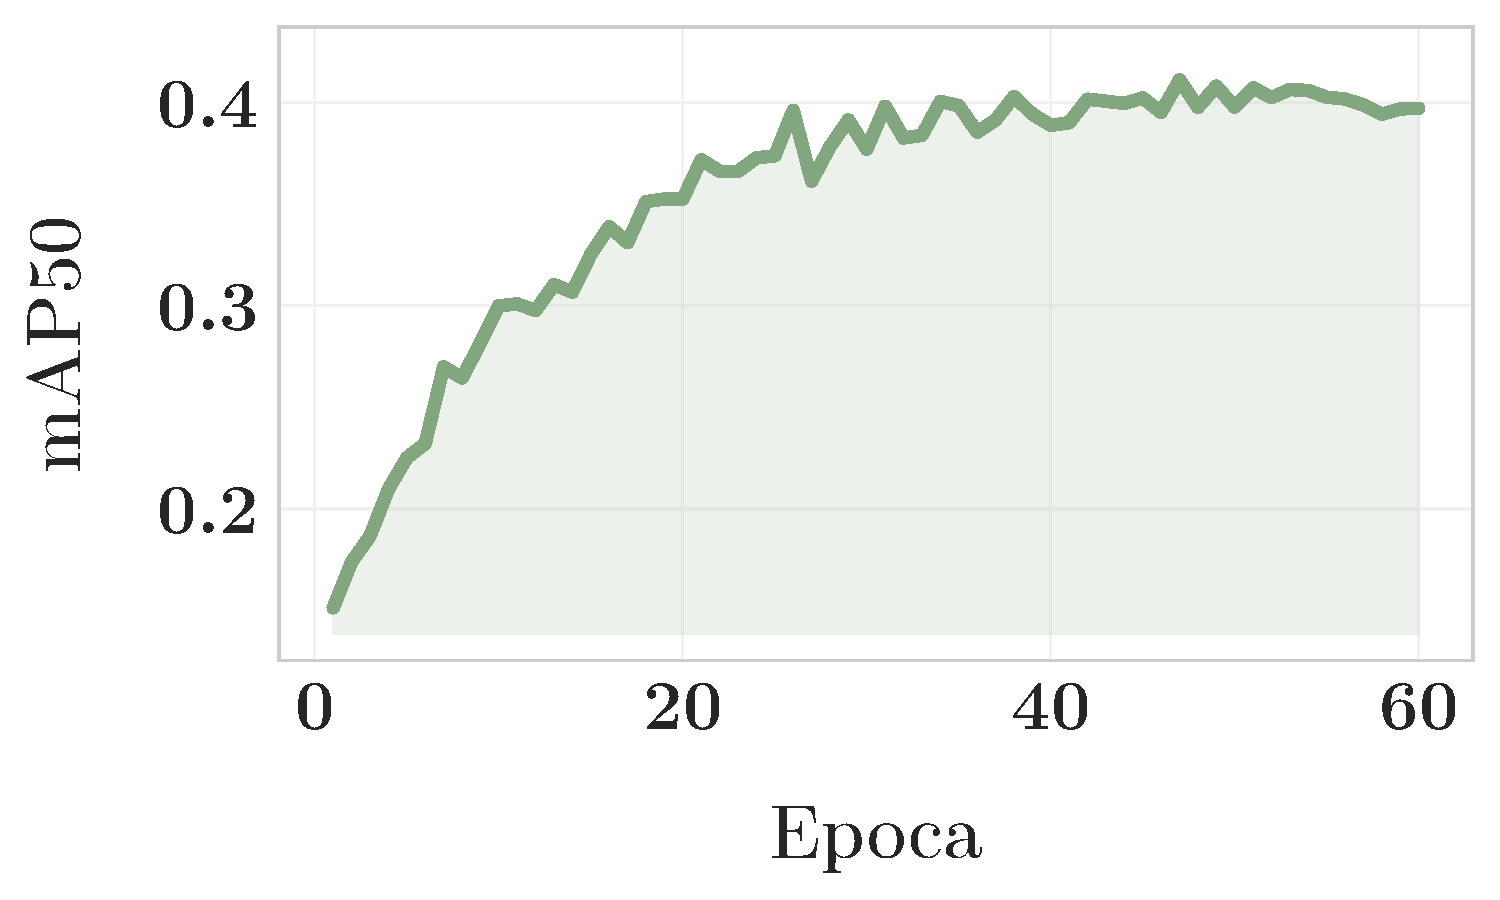
\includegraphics[width=0.48\textwidth]{images/domain-shift/real-to-real/6/map50}}
	\hspace{0.01\textwidth}
	{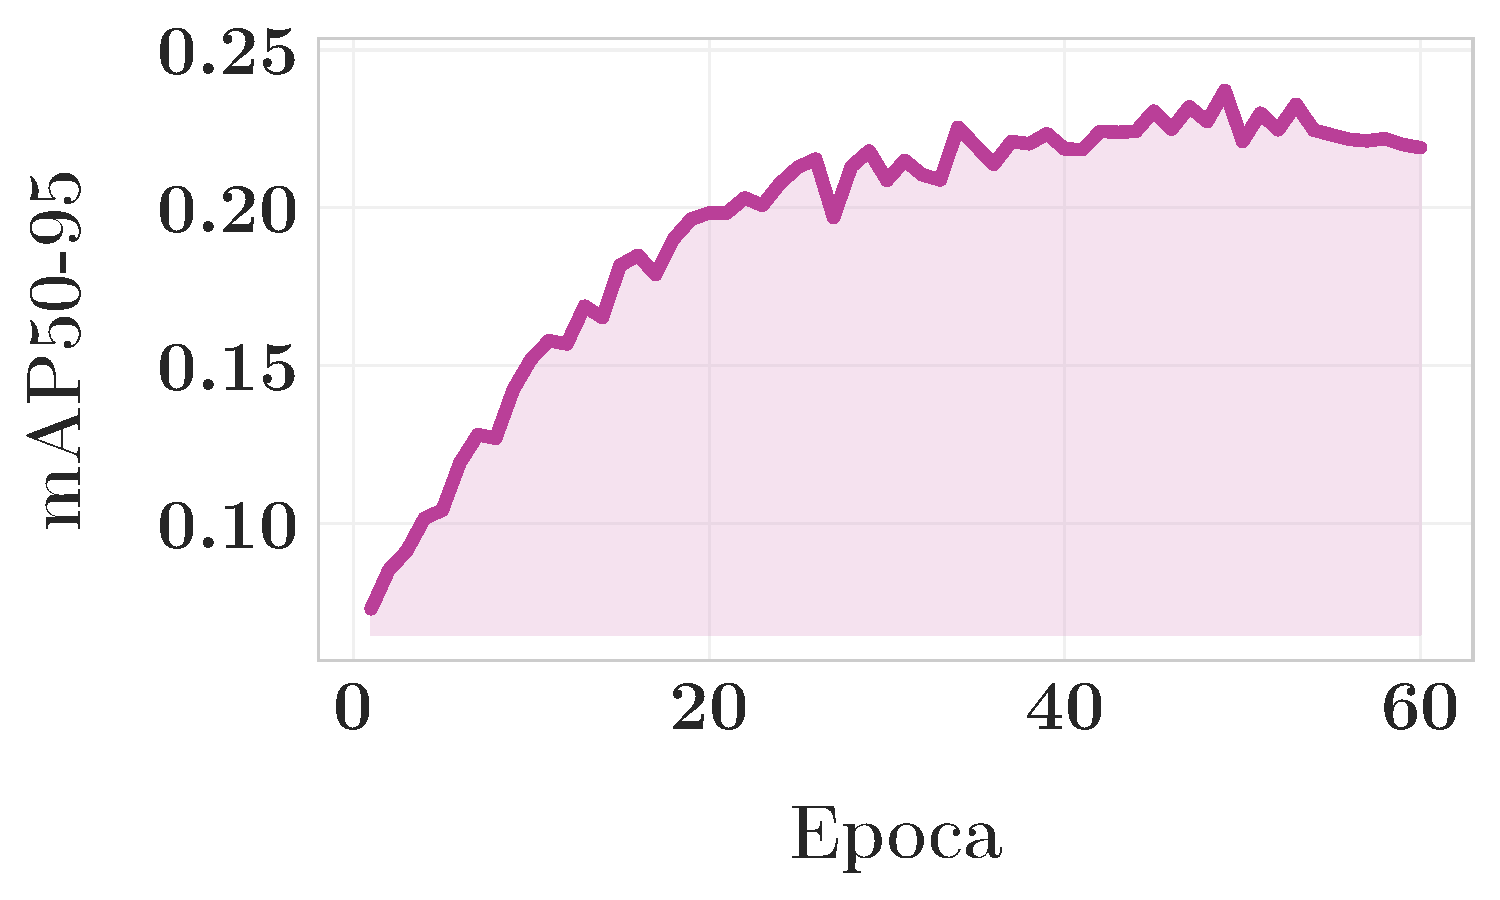
\includegraphics[width=0.48\textwidth]{images/domain-shift/real-to-real/6/map50-95}}
	\caption{Metriche di addestramento nel caso di 50 ambienti reali, con dati di testing provenienti da 20 diversi ambienti.}
	\label{fig:training-5}
\end{figure}

L'andamento dei grafici di loss risulta molto simile a quanto visto nell'esperimento precedente. La loss di training continua a calare quasi costantemente, mentre quella di testing, a partire dall'epoca 30, inizia ad aumentare, indicando un inizio di overfitting. Le cose invece sono diverse per quanto riguarda le metriche mAP. Nel suo picco massimo (epoca 47), la mAP50 raggiunge un valore di 0.411, mentre la mAP50-95 si attesta a 0.232. Questi valori sono quasi il doppio rispetto a quelli dell'esperimento precedente, evidenziando un notevole miglioramento delle prestazioni del modello.

Durante l'inferenza su immagini provenienti da ambienti reali, il modello dimostra di saper segmentare correttamente le classi di oggetti più rappresentate all'interno del dataset. Tra queste classi figurano: cabinet, chair, door, floor, monitor, picture e wall. Un esempio delle predizioni del modello è illustrato nella \hyperref[fig:prediciton-3]{Figura \ref{fig:prediciton-3}}.

\begin{figure}[h!]
	\centering
	{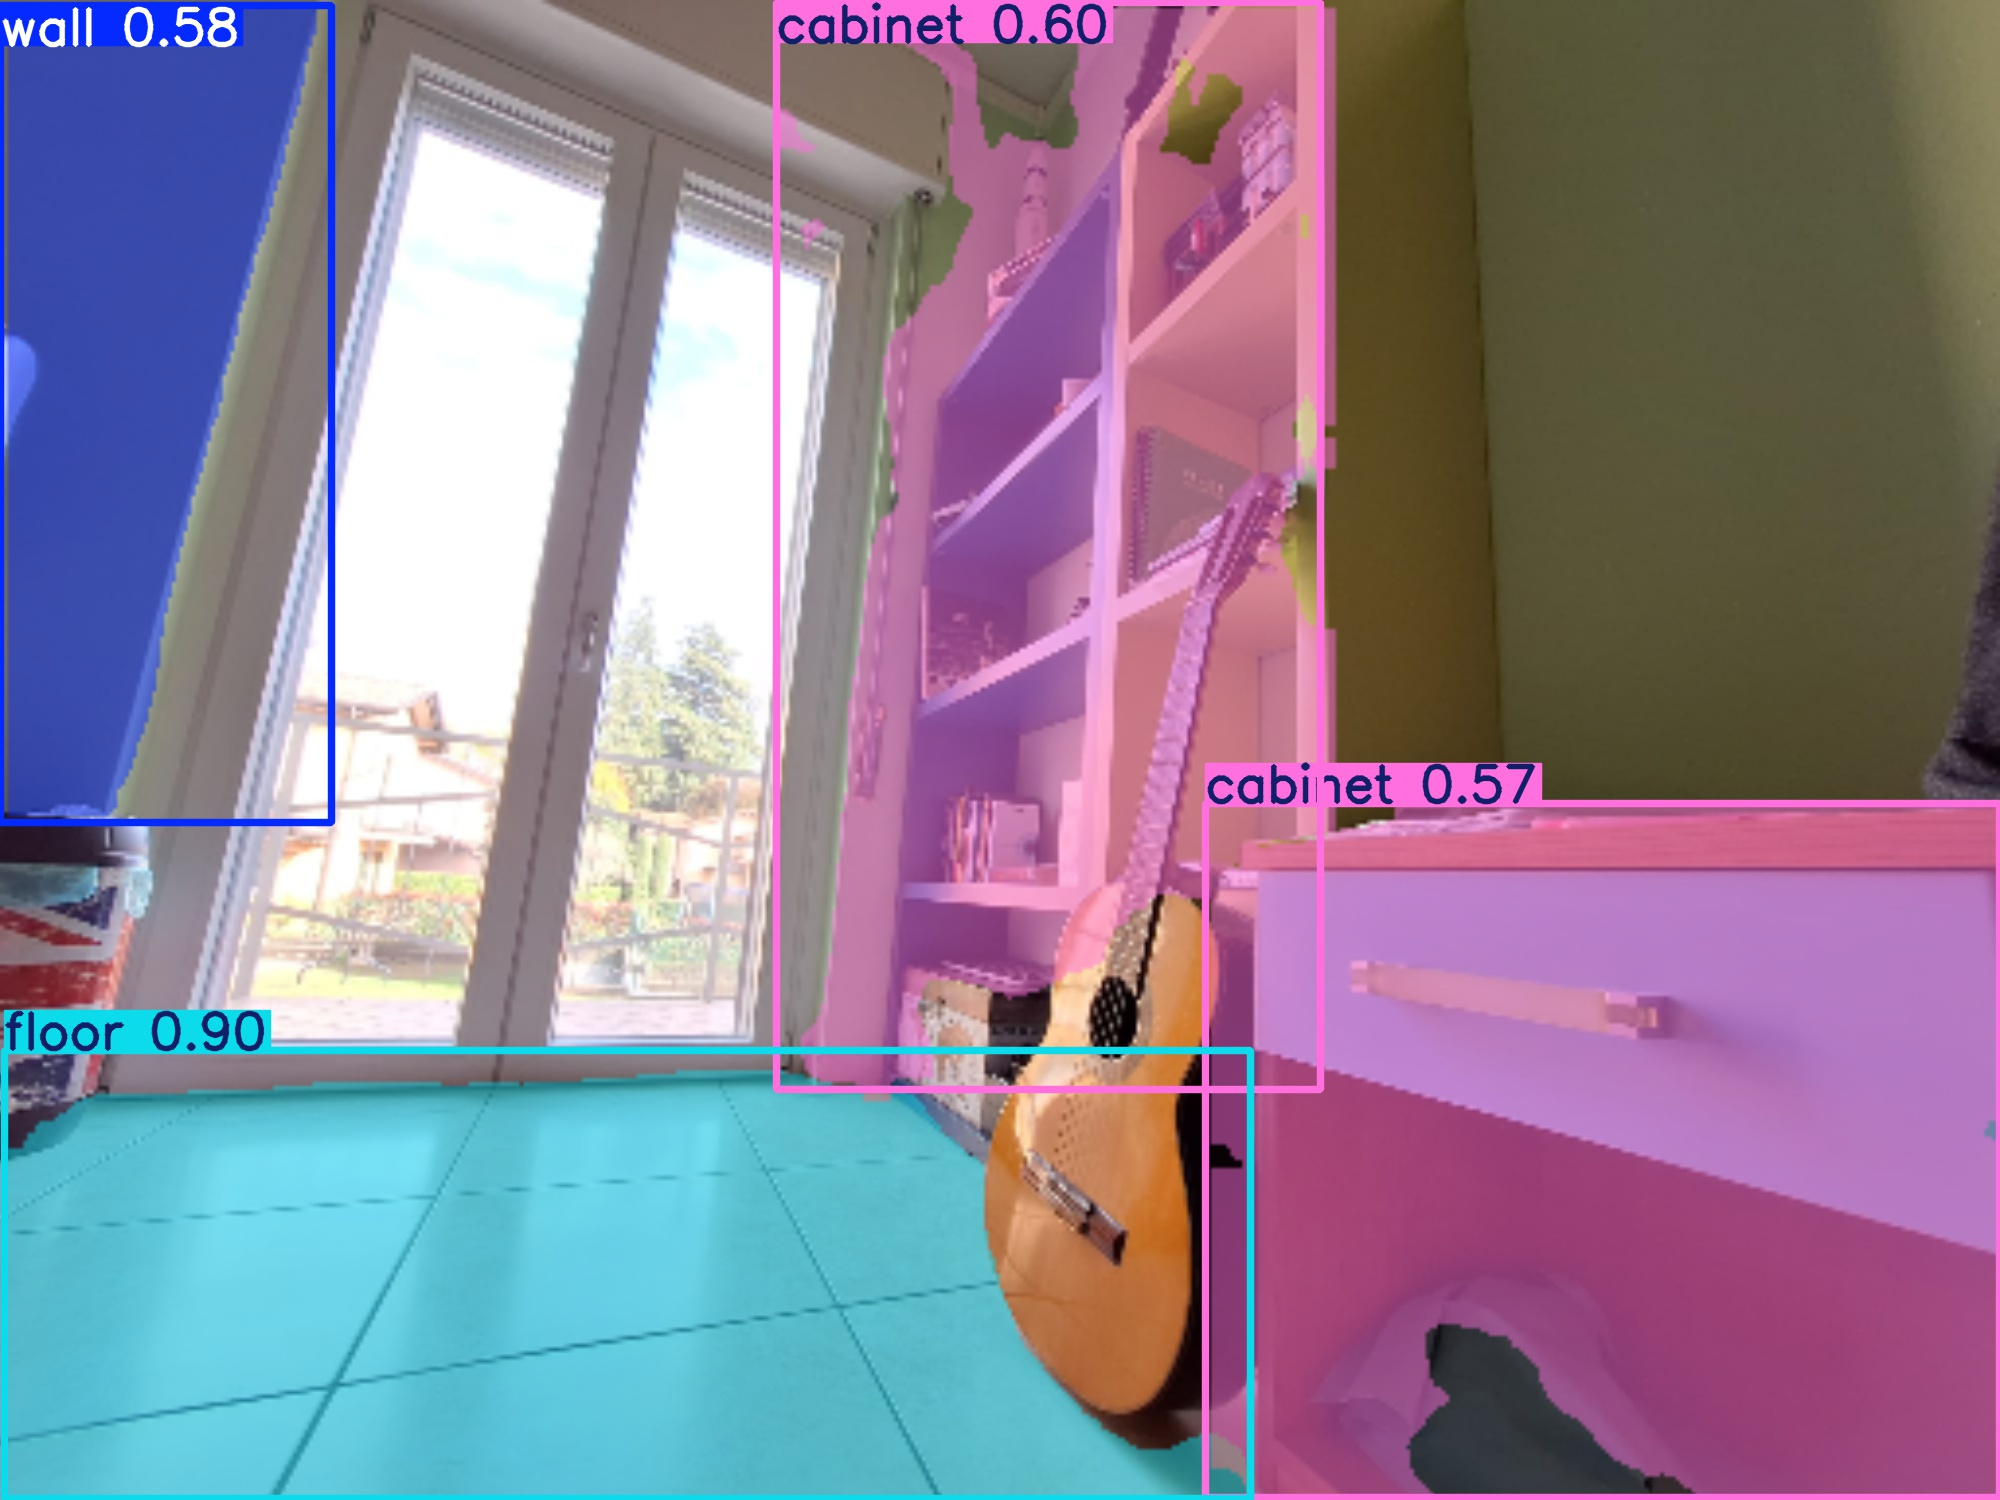
\includegraphics[width=0.42\textwidth]{images/domain-shift/real-to-real/6/prediction-1.jpg}}
	\hspace{0.01\textwidth}
	{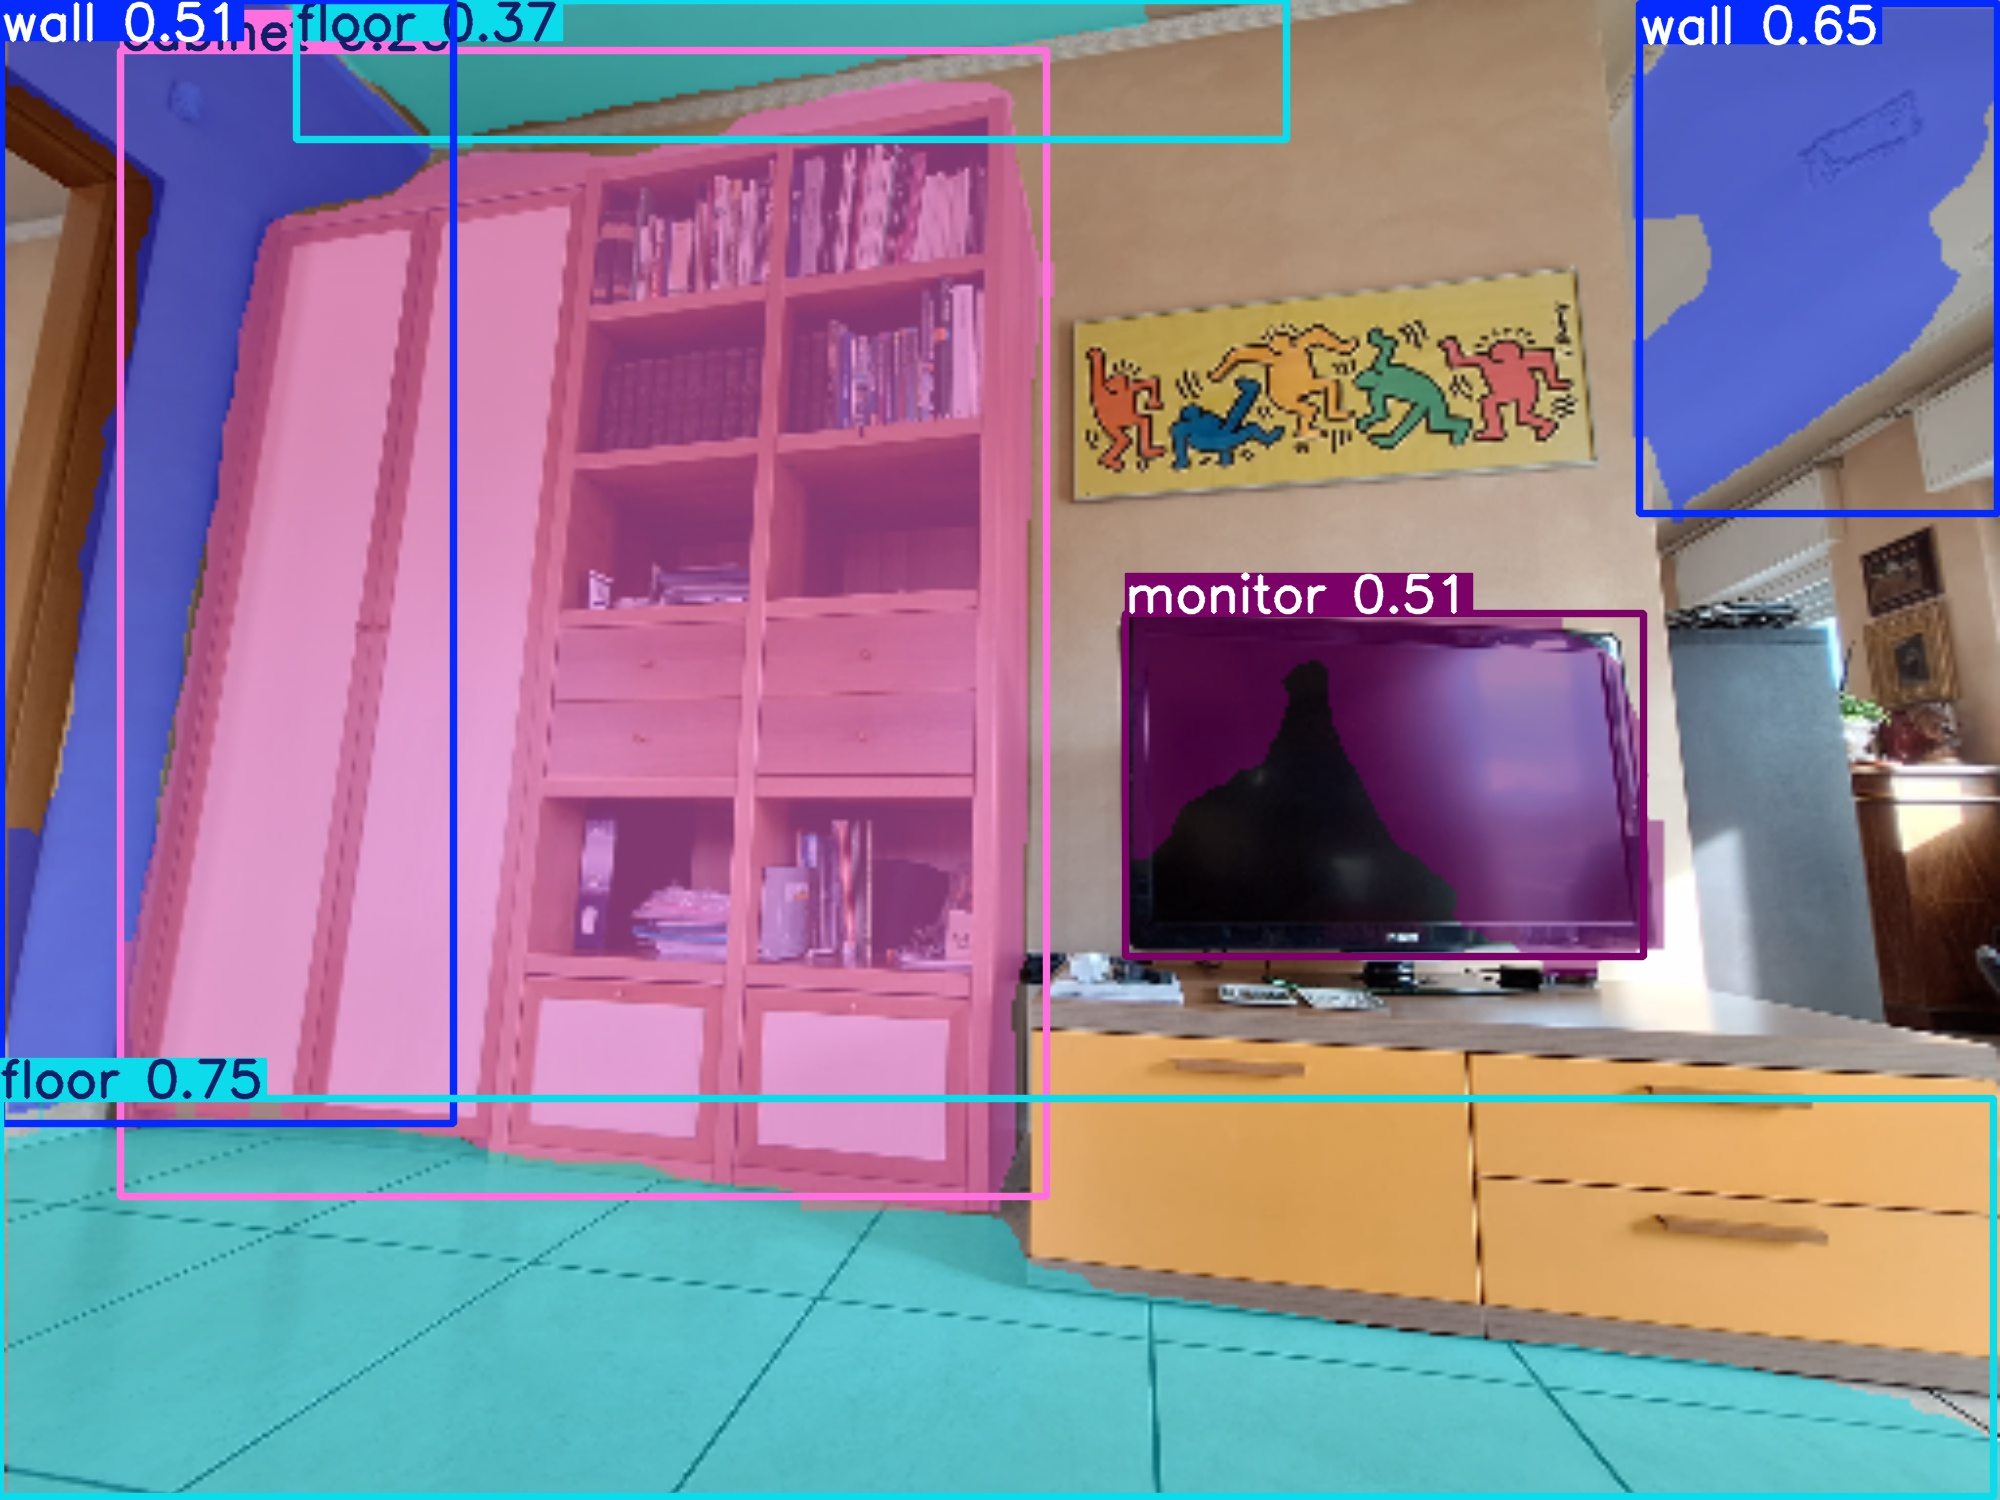
\includegraphics[width=0.42\textwidth]{images/domain-shift/real-to-real/6/prediction-2.jpg}}
	\caption{Predizioni del modello addestrato con 395 scene in un ambiente reale.}
	\label{fig:prediciton-3}
\end{figure}

Considerando i dati di validazione, questo modello ottiene una mAP50 di 0.459 e una mAP50-95 di 0.279. Questi valori sono molto vicini a quelli ottenuti in fase di training, con una differenza di 0.048 nel primo caso e 0.047 nel secondo. Questo risultato indica un domain shift di un ordine di grandezza inferiore rispetto a quanto osservato nell'\hyperref[sec:esperimento_5]{Esperimento 5} e nell'\hyperref[sec:esperimento_2]{Esperimento 2}. Questo dimostra che, per una generalizzazione efficace, è necessario disporre di dati eterogenei provenienti da un ampio numero di scene diverse tra loro. Inoltre, anche un numero limitato di immagini per ambiente è sufficiente a garantire una buona capacità di generalizzazione.

\subsection{Sim-to-real}
\label{sec:sim_to_real}

\subsubsection{Esperimento 7}
\label{sec:esperimento_7}

Infine, analizziamo il caso di studio sim-to-real, ovvero la capacità di un modello addestrato con dati simulati di generalizzare su dati reali. Per questo esperimento utilizziamo il modello dell'\hyperref[sec:esperimento_3]{Esperimento 3}, in quanto è stato addestrato con tutti e 15 gli ambienti disponibili. Questo lo distingue dagli esperimenti 1 e 2, nei quali tre ambienti sono stati utilizzati per il testing. Per valutare le performance si utilizza il modello YOLO11 preaddestrato e il dataset contenente immagini reali con le relative annotazioni di segmantazione. In particolare sono state utilizzate le stesse 1000 immagini provenienti dalle 20 scene utilizzate nella sezione real-to-real. Il risultato finale indica una  mAP50 pari a 0.015 e una mAP50-95 di 0.007, il che conferma le seguenti ipotesi:

\begin{enumerate}
	\item Non è importante la quantità di immagini impiegate, ma conta il numero di ambienti utilizzati e il loro livello di ererogeneità.
	
	\item Le limitazioni del simulatore fanno sì che risulta impossibile trasferire le conoscenze acquisite da un ambiente simulato a uno reale. 
\end{enumerate}

D'altro canto, questi risultati erano prevedibili alla luce dei dati ottenuti nell'\hyperref[sec:esperimento_2]{Esperimento 2}, dove, pur restando nel dominio della simulazione e cambiando solo gli ambienti, si aveva una riduzione di entrambe le mAP di circa 0.4. Di conseguenza, passando dalla simulazione al mondo reale performance non potevano che deteriorare, e questi risultati lo dimostrano. Inoltre, la scarsa eterogeneità degli ambienti ha contribuito a peggiorare ulteriormente i risultati.

\section{Domain adaptation in fog robotics}
\label{sec:domain_shift_in_contesto_fog_robotics}

In questa sezione si utilizza l'architettura UNet-YOLO implementata nel \hyperref[chap:metodo]{Capitolo \ref{chap:metodo}} per cercare di mitigare il fenomeno del domain shift in un sistema fog robotics. Gli scenari considerati riguardano sia il caso real-to-real che sim-to-real.

\subsection{Real-to-real}
\label{sec:real_to_real_fr}

Questa serie di esperimenti valuta le prestazioni dell'architettura UNet-YOLO in un sistema fog robotics, utilizzando come dominio sorgente e target ambienti reali. In particolare si considera una situazione nella quale si ha un segmentatore semantico pre-addestrato con dati reali provenienti da 395 ambienti, utilizzando poi una piccola quantità di dati raccolti nel dominio di destinazione per effettuare un fine-tuning dell'encoder-decoder e del segmentatore.

Per questi esperimenti, il segmentatore semantico utilizzato corrisponde al modello ottenuto all’epoca 47 nell'\hyperref[sec:esperimento_5]{Esperimento 5}, mentre i pesi della UNet vengono inizializzati ex novo all'inizio di ogni sessione di addestramento.

\subsubsection{Esperimento 8}
\label{sec:esperimento_8}

In questo primo esperimento sono state utilizzate 1000 immagini per il fine-tuning provenienti da 20 scene, diverse dalle 395 utilizzate per addestrate il segmentatore. Le prestazioni del modello sono state successivamente valutate su 175 immagini di validazione, anch'esse provenienti dalle stesse 20 scene. Nonostante sia stata utilizzata la macchina più potente a disposizione, le risorse hardware erano appena sufficienti per effettuare l'addestramento. Il training ha richiesto il caricamento in VRAM sia del modello UNet che di YOLO, e questo ha limitato il batch size ad 1, mantenendo la risoluzione delle immagini a 640 pixel. L'intero processo di addestramento è durato circa 5 ore.

L'opzione di utilizzare più immagini immagini per il training è stata presa in considerazione, ma avrebbe causato un notevole aumento dei tempi di addestramento. Inoltre, trattandosi di fine-tuning, l'uso di una piccola quantità di dati si è rivelata una scelta più coerente con quello che è lo scopo dell'esperimento. Le metriche ottenute alla fine del training sono illustrate nella \hyperref[fig:training-6]{Figura \ref{fig:training-6}}.

\begin{figure}[h!]
	\centering
	{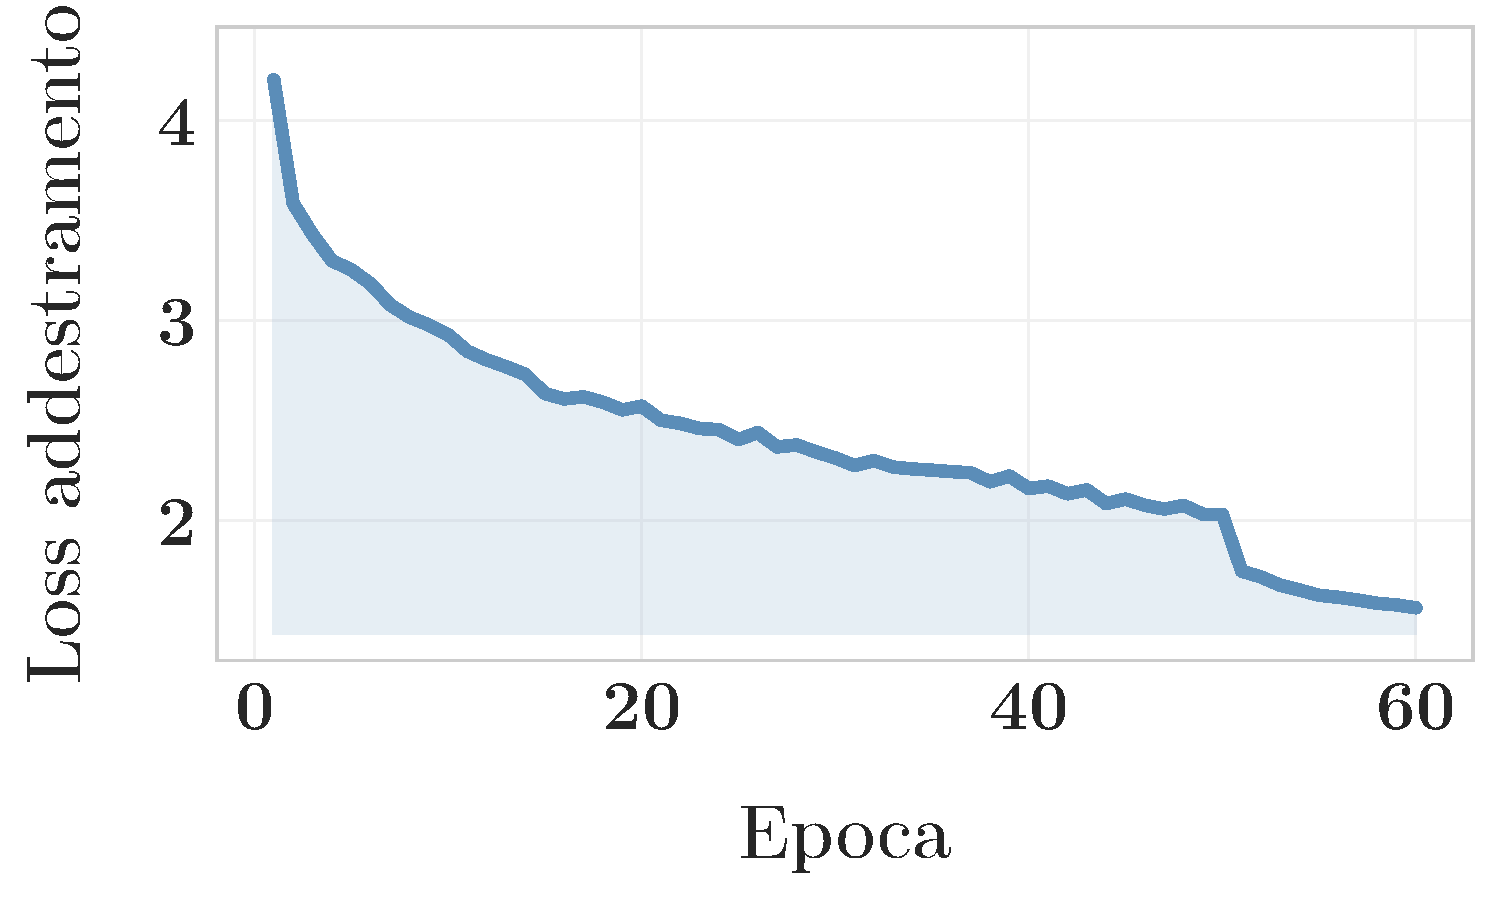
\includegraphics[width=0.48\textwidth]{images/fog-robotics/real-to-real/8/train-loss}}
	\hspace{0.01\textwidth}
	{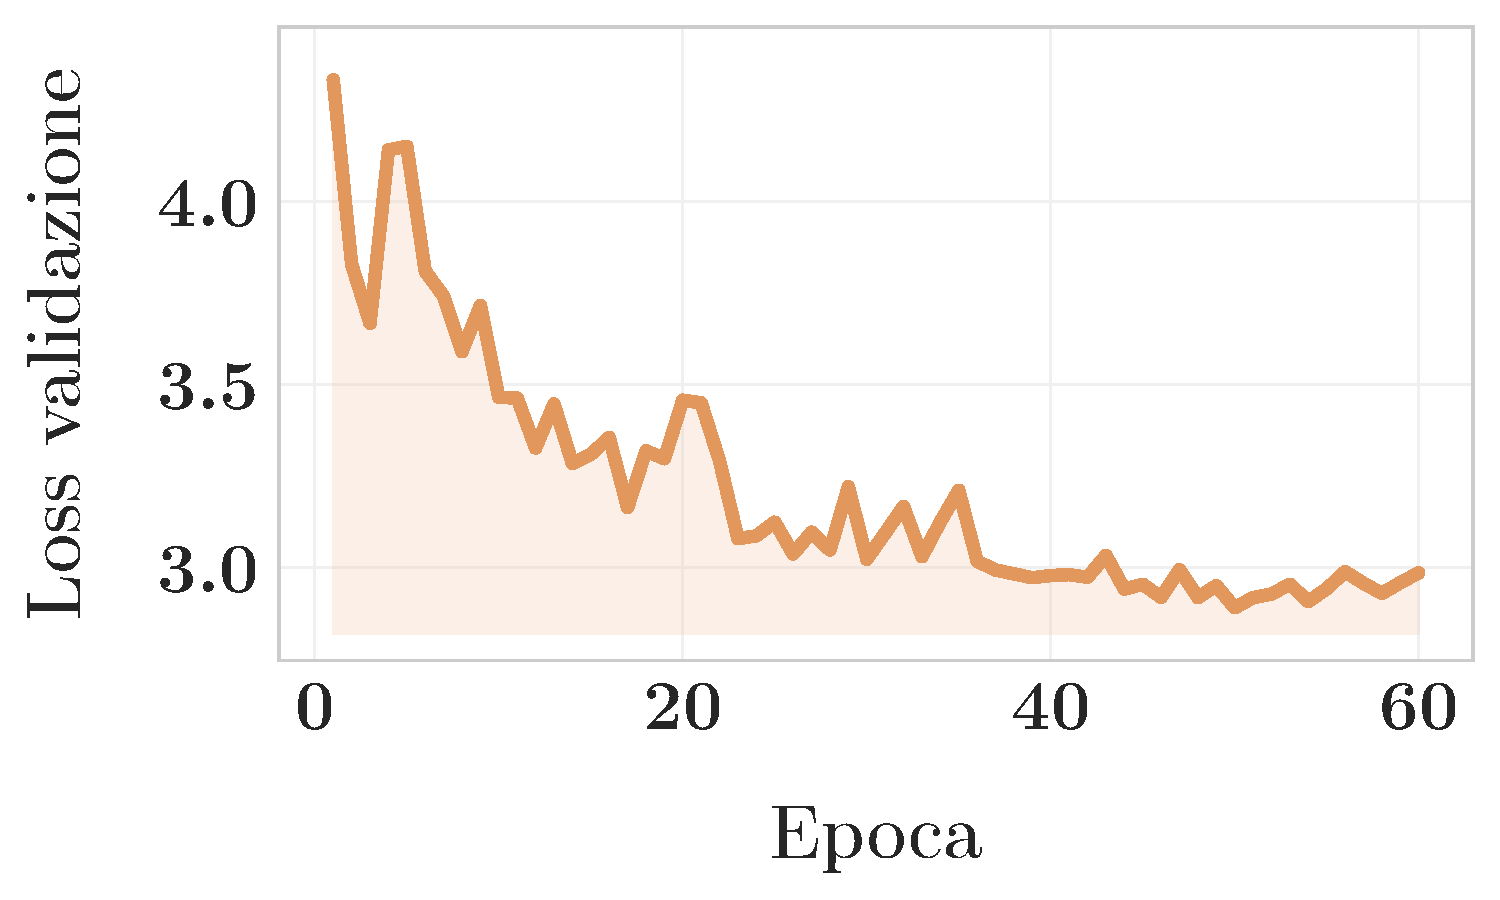
\includegraphics[width=0.48\textwidth]{images/fog-robotics/real-to-real/8/validation-loss}}
	\hspace{0.01\textwidth}
	\\
	{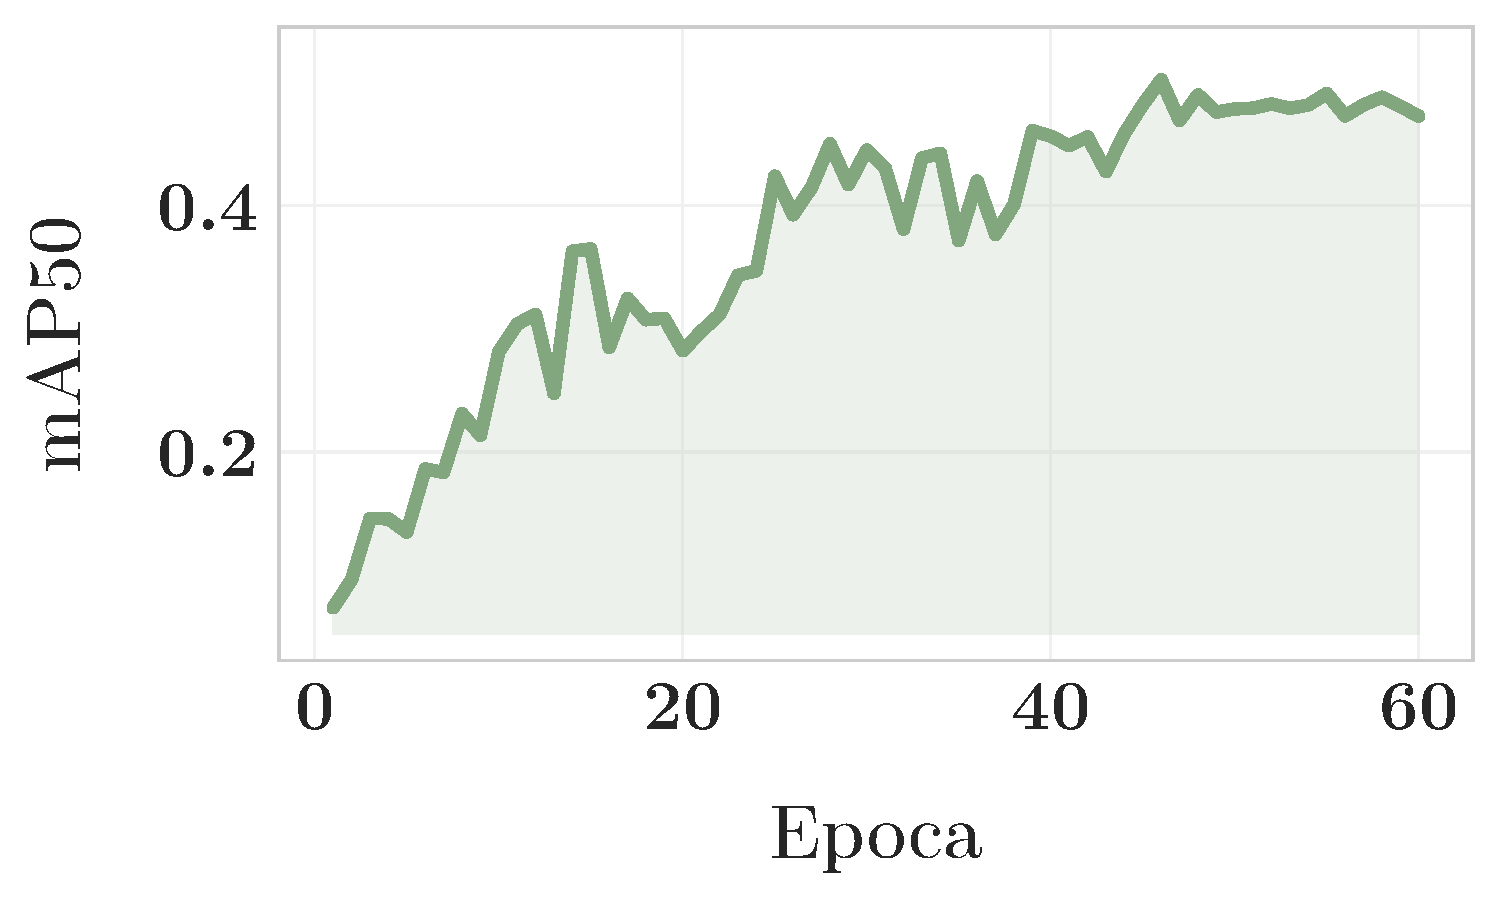
\includegraphics[width=0.48\textwidth]{images/fog-robotics/real-to-real/8/map50}}
	\hspace{0.01\textwidth}
	{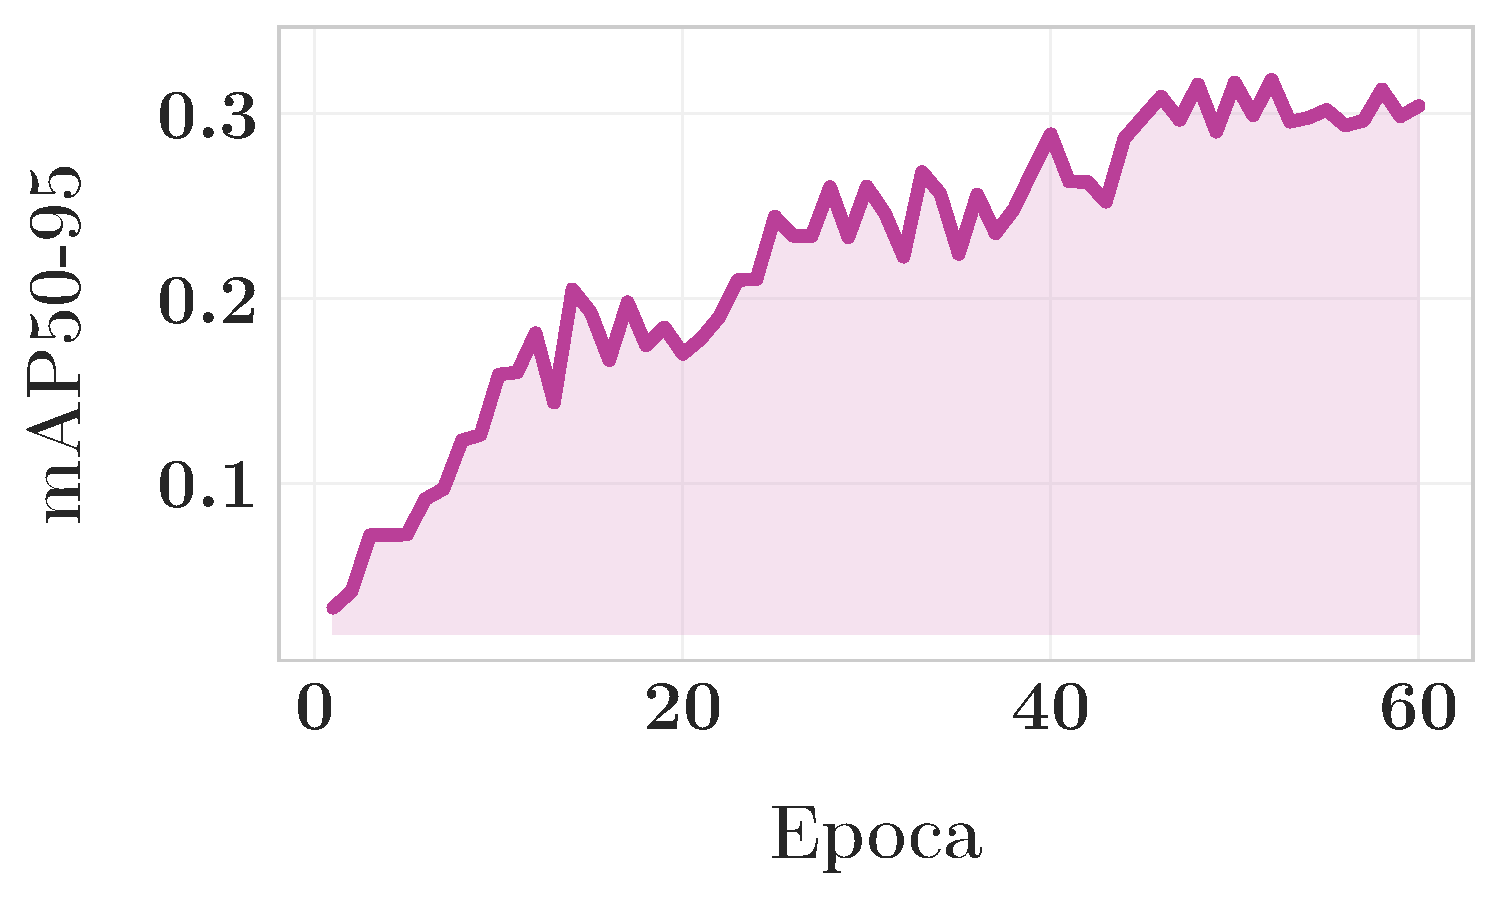
\includegraphics[width=0.48\textwidth]{images/fog-robotics/real-to-real/8/map50-95}}
	\caption{Metriche di addestramento del modello distribuito, utilizzando un segmentatore preaddestrato con 395 scene. Fine-tuning e validazione effettuati con dati provenienti da altre 20 scene.}
	\label{fig:training-6}
\end{figure}

Dai risultati ottenuti si nota che il modello riesce ad adattarsi in al nuovo dominio senza presentare segni di overfitting. Le mAP sono sufficientemente alte, con la mAP50 che nel picco più alto si attesta a 0.502 e la mAP50-95 a 0.309. È inoltre interessare analizzare come la UNet trasforma l'immagine prima di inviarla al segmentatore semantico. Nella \hyperref[fig:prediciton-4]{Figura \ref{fig:prediciton-4}} è mostrata un'immagine di input ricevuta dall'encoder-decoder, e il corrispettivo output.

\begin{figure}[h!]
	\centering
	\subfloat[]{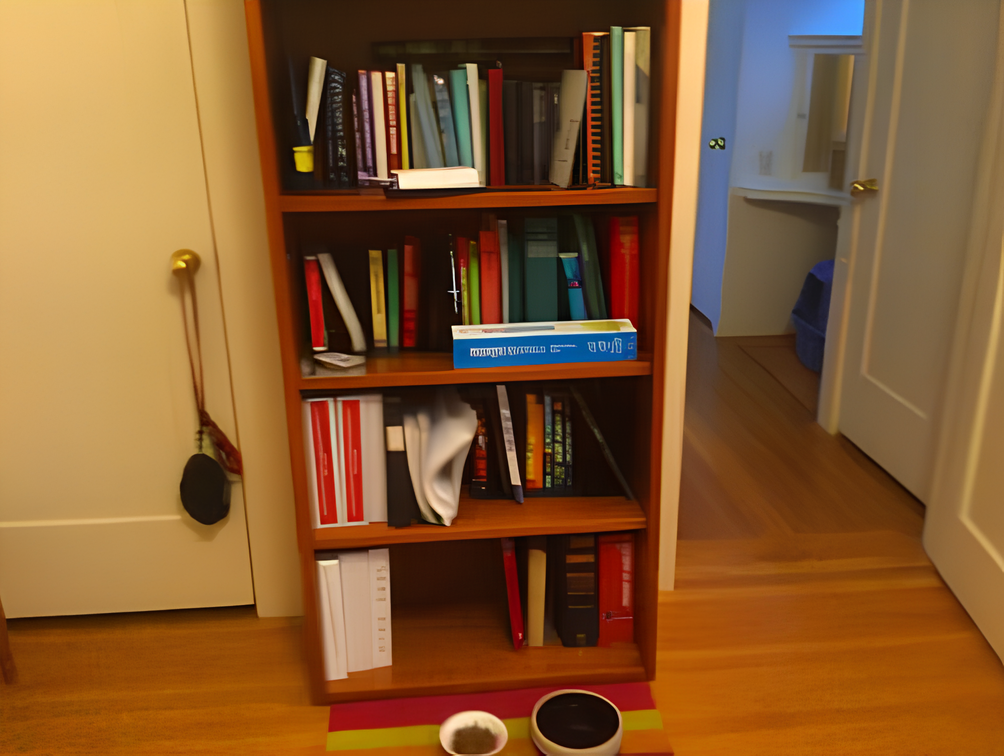
\includegraphics[width=0.42\textwidth]{images/fog-robotics/real-to-real/8/input.png}}
	\hspace{0.01\textwidth}
	\subfloat[]{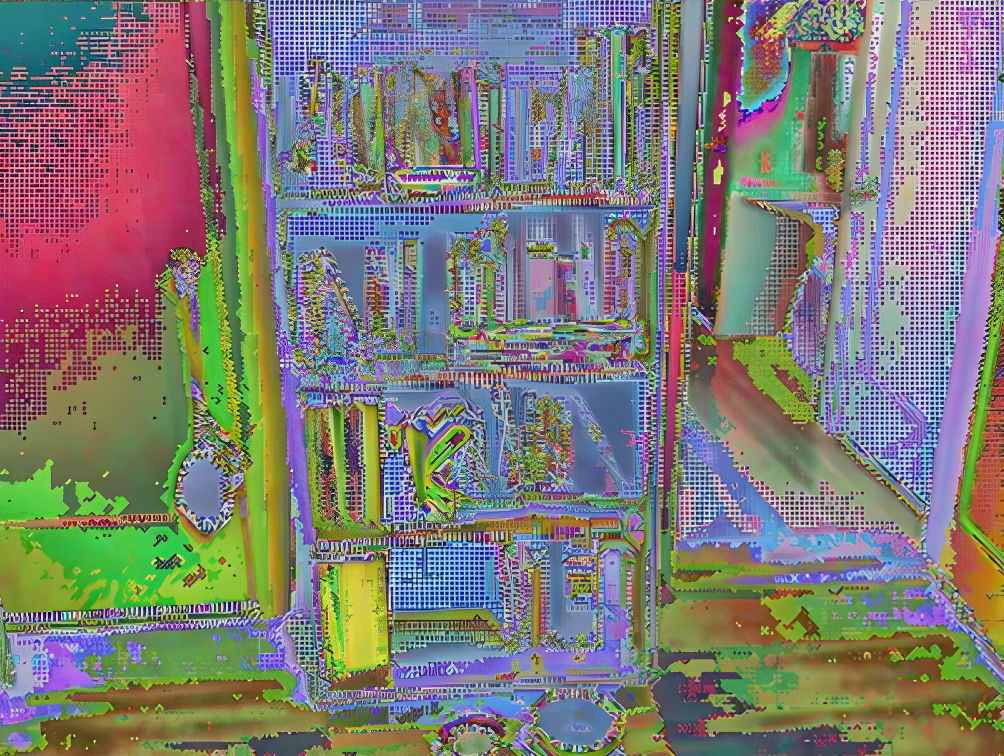
\includegraphics[width=0.42\textwidth]{images/fog-robotics/real-to-real/8/output.png}}
	\caption{Input (a) e output (b) della UNet.}
	\label{fig:prediciton-4}
\end{figure}

\subsubsection{Esperimento 9}
\label{sec:esperimento_9}

Nel seguente esperimento valuteremo invece le performance della stessa architettura riducendo il numero di parametri della UNet. Partendo dai 31 milioni di parametri originali, sono state ridodde le dimensioni del modello fino a raggiungere quota 7.7 milioni di parametri. Lo scopo è verificare se la UNet è in grado di mantenere un buon equilibrio tra prestazioni ed efficienza, riducendo al contempo il carico di lavoro sui server fog. Tutti gli altri parametri e i dataset restano invariati rispetto all'esperimento precedente, tranne la macchina sulla quale è stato eseguito che è la PC2. Dopo 26 ore di addestramento, i risultati ottenuti sono riportati nella \hyperref[fig:training-7]{Figura \ref{fig:training-7}}.

\begin{figure}[h!]
	\centering
	{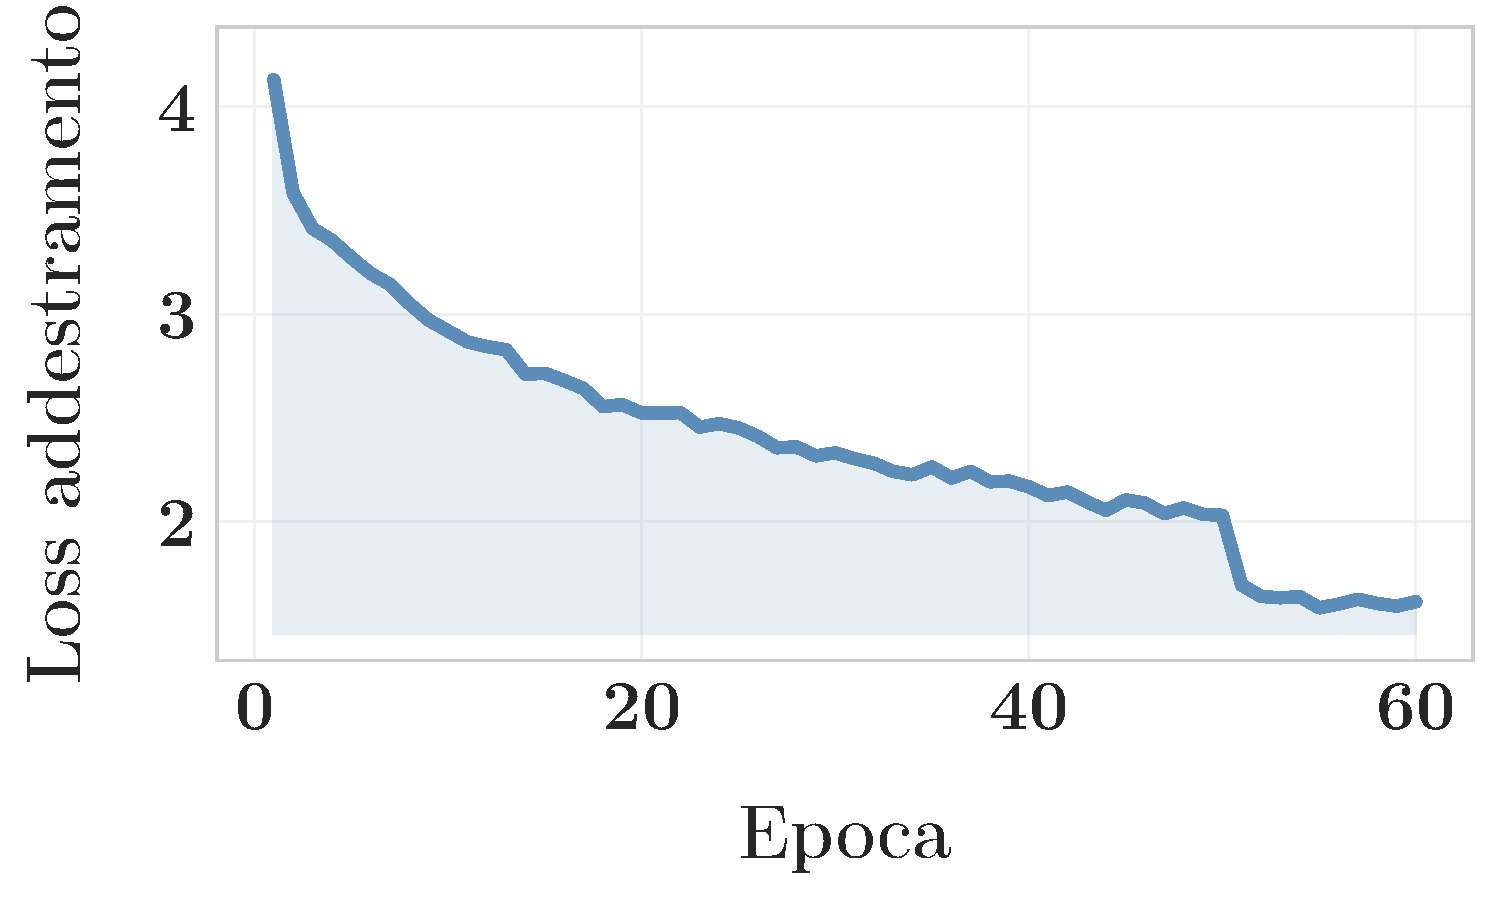
\includegraphics[width=0.48\textwidth]{images/fog-robotics/real-to-real/9/train-loss}}
	\hspace{0.01\textwidth}
	{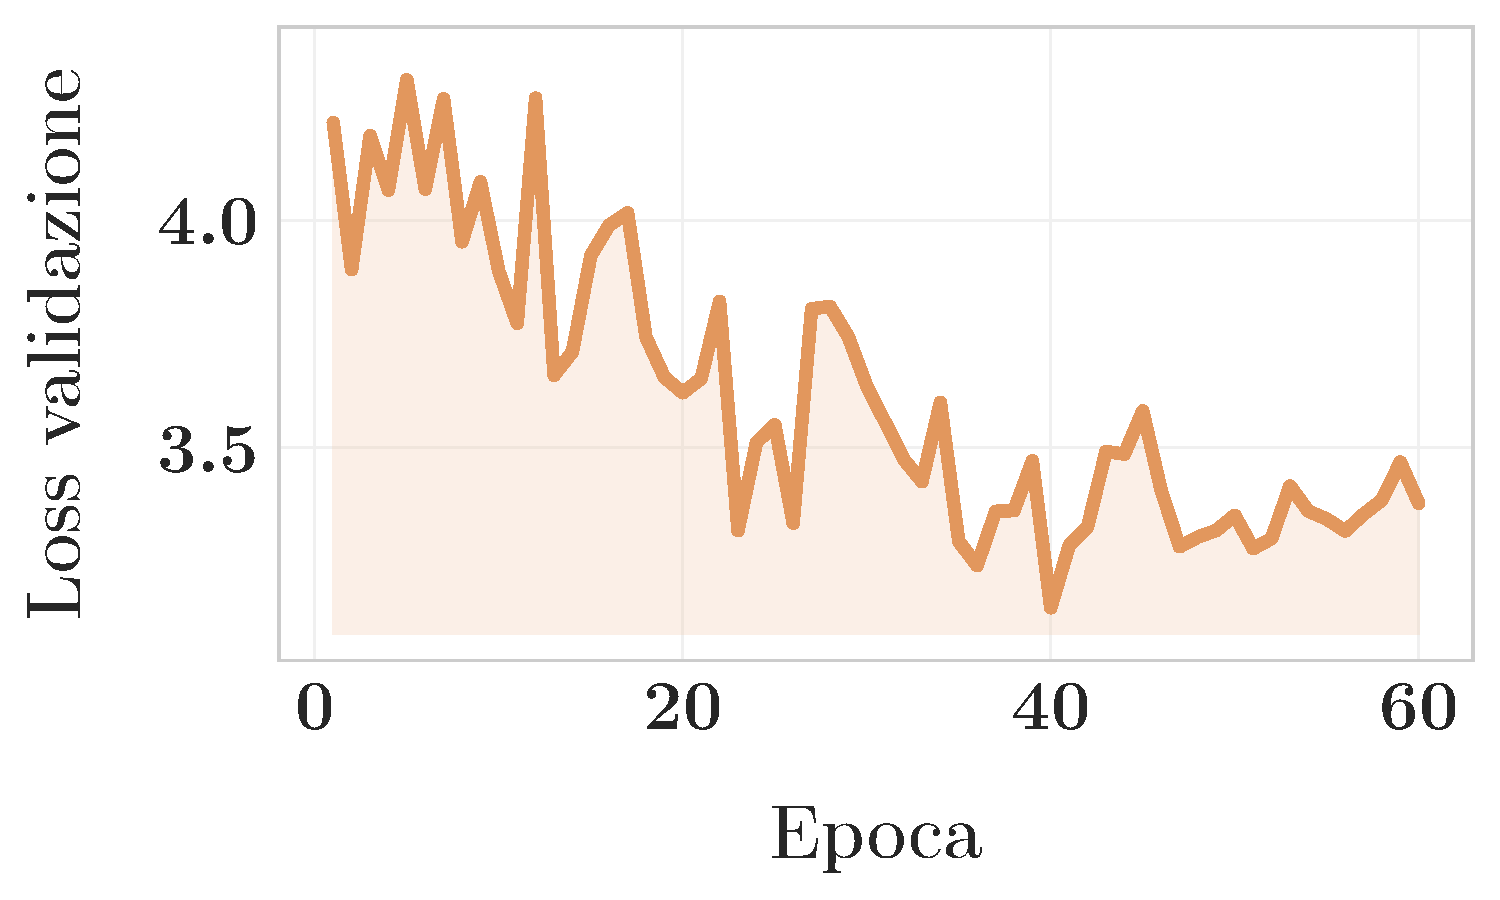
\includegraphics[width=0.48\textwidth]{images/fog-robotics/real-to-real/9/validation-loss}}
	\hspace{0.01\textwidth}
	\\
	{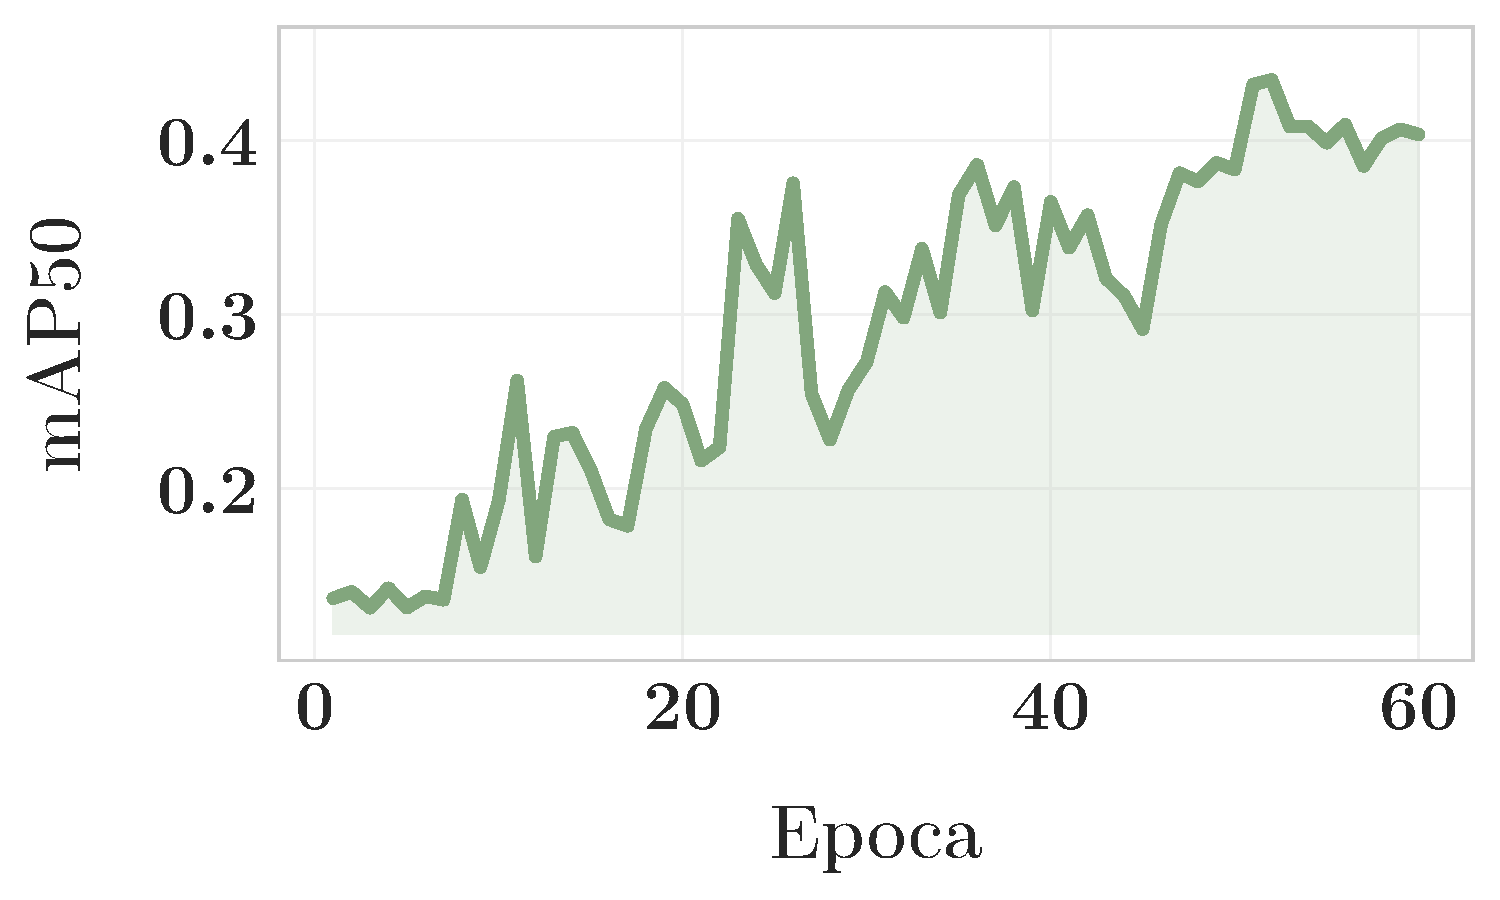
\includegraphics[width=0.48\textwidth]{images/fog-robotics/real-to-real/9/map50}}
	\hspace{0.01\textwidth}
	{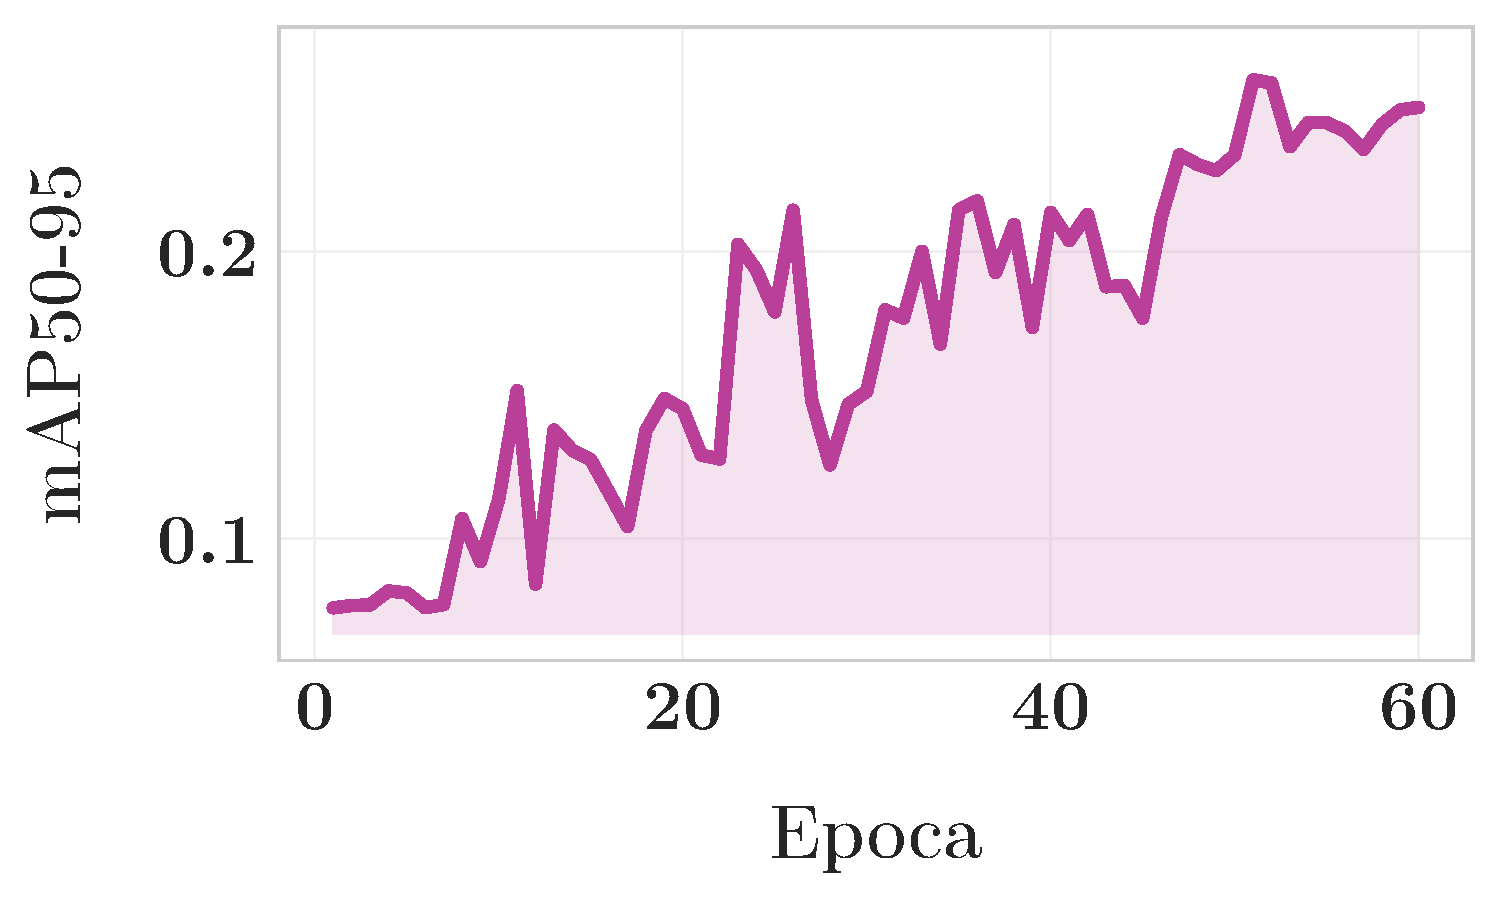
\includegraphics[width=0.48\textwidth]{images/fog-robotics/real-to-real/9/map50-95}}
	\caption{Metriche di addestramento del modello distribuito, utilizzando un segmentatore pre-addestrato con 395 scene. Fine-tuning e validazione effettuati con dati provenienti da altre 20 scene. È stata utilizzata una UNet con solo 7.7 milioni di parametri.}
	\label{fig:training-7}
\end{figure}

Questi risultati differiscono da quelli ottenuti lo scorso esperimento. Si nota infatti che, utilizzando un numero ridotto di parametri, la loss di validazione diminuisce in modo irregolare e rumoroso. Lo stesso comportamento vale per le mAP, che mostrano un aumento ma con una certa variabilità. In genere questo può avvenire nel caso di batch size troppo piccoli o quando i dati di training presentano un'elevata variabilità. Non è però questo il caso, poichè l'esperimento è stato riprodotto con gli stessi dati del precedente. L'unica soluzione plausibile è che sia causato dal numero piccolo di parametri.

Nonstante ciò, i risultati ottenuti restano comunque soddisfacenti: la mAP50 è pari a 0.435 mentre la mAP50-95 è di 0.259. Considerando una riduzione di circa il 75\% dei parametri della UNet, questa soluzione potrebbe rappresentare un'ottima alternativa per sistemi fog con risorse limitate. Per tutti i restanti esperimenti si continuerà ad usare la UNet da 31 milioni di parametri.

\subsubsection{Esperimento 10}
\label{sec:esperimento_10}

Per l'ultimo esperimento della sezione real-to-real si è infine provato ad addestrare la UNet congelando i pesi del segmentatore semantico. Con questo test si è voluto valutare quanto la UNet fosse flessibile ad adattare il dominio destinazione a quello sorgente, senza andare a modificare i parametri di YOLO11. L'addestramento è stato eseguito sulla macchina PC1, e tutti gli altri parametri sono rimasti invariati rispetto all'\hyperref[sec:esperimento_8]{Esperimento 8}. Nella \hyperref[fig:training-8]{Figura \ref{fig:training-8}} sono illustrati i risultati.

\begin{figure}[h!]
	\centering
	{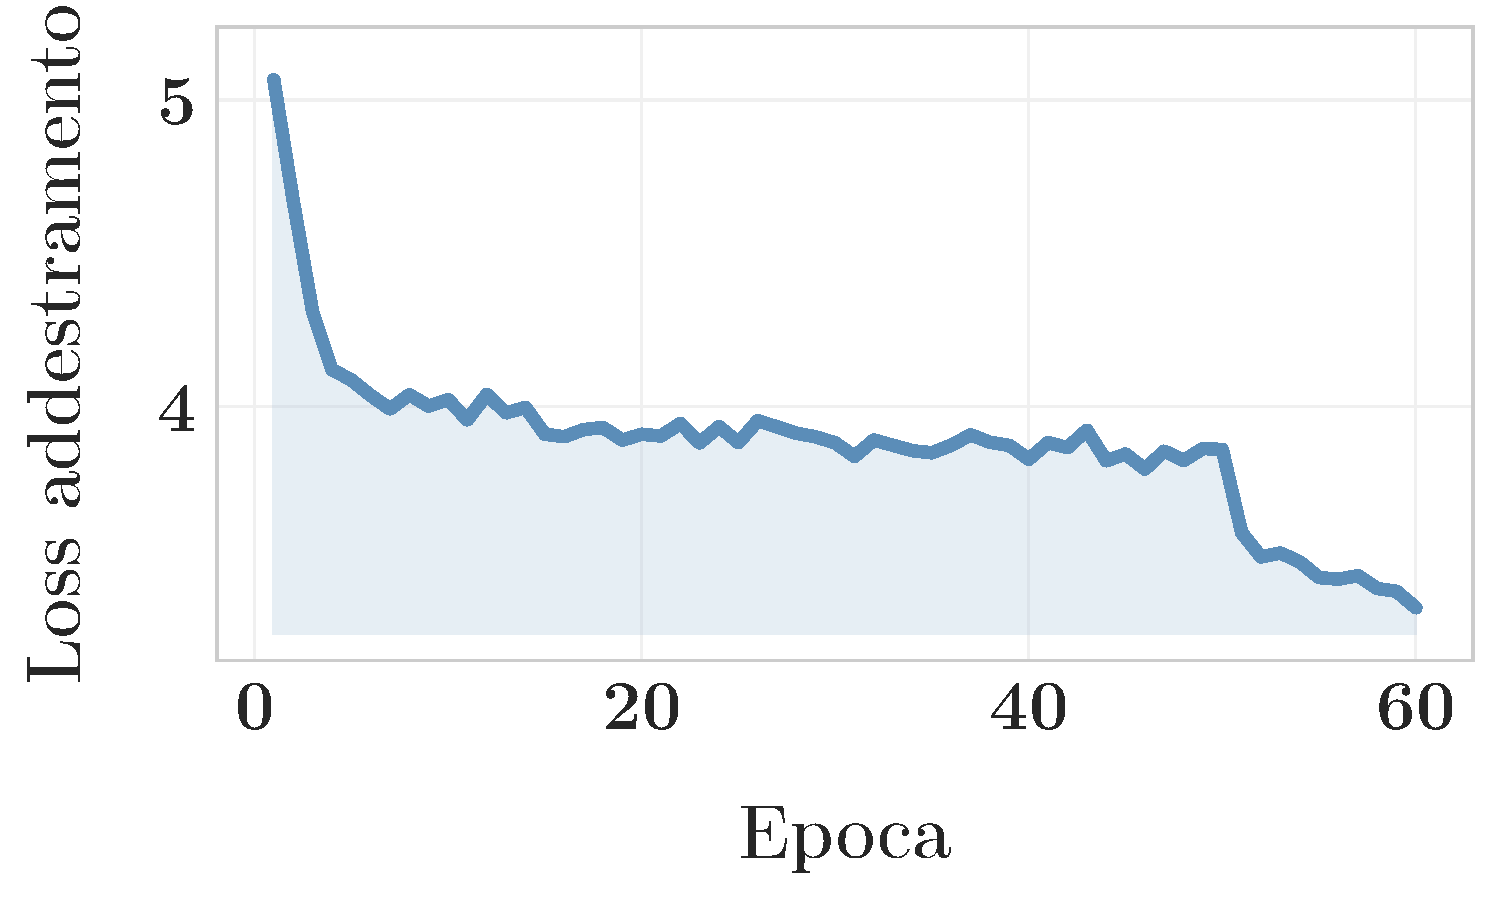
\includegraphics[width=0.48\textwidth]{images/fog-robotics/real-to-real/10/train-loss}}
	\hspace{0.01\textwidth}
	{\includegraphics[width=0.48\textwidth]{images/fog-robotics/real-to-real/10/validation-loss}}
	\hspace{0.01\textwidth}
	\\
	{\includegraphics[width=0.48\textwidth]{images/fog-robotics/real-to-real/10/map50}}
	\hspace{0.01\textwidth}
	{\includegraphics[width=0.48\textwidth]{images/fog-robotics/real-to-real/10/map50-95}}
	\caption{Metriche di addestramento del modello distribuito, utilizzando un segmentatore pre-addestrato con 395 scene. Addestramento e validazione effettuati con dati provenienti da altre 20 scene. I pesi del segmentatore semantico sono stati congelati.}
	\label{fig:training-8}
\end{figure}

Come mostrato dai grafici, la UNet da sola non è in grado di proiettare correttamente le immagini del dominio target su quello di addestramento. Per ottenere questo risultato, è necessario co-addestrare entrambi i modelli. Di conseguenza l'encoder-decoder non impara nulla e i valori delle mAP restano prossimi allo zero durante tutto il processo di training.

\subsection{Sim-to-real}
\label{sec:sim_to_real_fr}

\subsubsection{Esperimento 11}
\label{sec:esperimento_11}

Come ultimo esperimento di questo elaborato, analizziamo la capacità dell'architettura UNet-YOLO di proiettare i dati provenienti dal mondo reale nel dominio del segmentatore semantico, addestrato su dati simulati. In particolare, l'obiettivo è far sì che la UNet trasformi le feature delle immagini reali nelle corrispondenti feature presenti negli ambienti simulati. Per fare questo utilizziamo il modello YOLO11 ottenuto nell'\hyperref[sec:esperimento_3]{Esperimento 3} e, senza congelare i suoi pesi, effettuiamo fine-tuning con le stesse 20 scene utilizzate in precedenza. A causa delle limitate risorse hardware, anche per questo esperimento si è costretti ad impostare ad 1 la dimensione del batch, lasciando tutti gli altri parametri inalterati rispetto agli esperimenti precedenti. L'addestramento è stato eseguito su PC1 e, dopo circa 5 ore, sono state prodotte le metriche riportate nella \hyperref[fig:training-9]{Figura \ref{fig:training-9}}.

\begin{figure}[h!]
	\centering
	{\includegraphics[width=0.48\textwidth]{images/fog-robotics/sim-to-real/11/train-loss}}
	\hspace{0.01\textwidth}
	{\includegraphics[width=0.48\textwidth]{images/fog-robotics/sim-to-real/11/validation-loss}}
	\hspace{0.01\textwidth}
	\\
	{\includegraphics[width=0.48\textwidth]{images/fog-robotics/sim-to-real/11/map50}}
	\hspace{0.01\textwidth}
	{\includegraphics[width=0.48\textwidth]{images/fog-robotics/sim-to-real/11/map50-95}}
	\caption{Metriche di addestramento del modello distribuito, utilizzando un segmentatore pre-addestrato con 15 scene simulate. Addestramento e validazione effettuati con dati provenienti da 20 scene reali.}
	\label{fig:training-9}
\end{figure}

Dall'analisi dei grafici si nota come il modello UNet-YOLO non riesca a trasformare le feature provenienti dagli ambienti reali in caratteristiche comprensibili dal segmentatore semantico. ntrambe le metriche mAP restano infatti prossime allo zero per l'intero periodo di addestramento. La causa più probabile a questo problema potrebbe essere la troppa differenza tra le immagini dei due domini. Nell'\hyperref[sec:esperimento_8]{Esperimento 8} il domain shift tra gli ambienti è più contenuto, permettendo al modello di compensare e adattarsi. In questo caso, invece, l'architettura utilizzata non è sufficientemente complessa per gestire questo maggiore domain shift. Per migliorare i risultati sono possibili due soluzioni. La prima consiste nell'utilizzare un simulatore più fotorealistico, così da diminuire il gap tra i domini. L'altra opzione è invece utilizzare un encoder-decoder più complesso, in modo da riuscire a colmare un gap più grande tra i due domini.

% CAPITOLO 6: Conclusioni
\chapter{Conclusioni}
\label{chap:conclusioni}

In questo elaborato si è analizzato il fenomeno del domain shift in diversi scenari, e si è realizzata un'architettura per ridurre il domain shift in un sistema di fog robotics.

I risultati ottenuti evidenziano che un segmentatore validato sugli stessi ambienti utilizzati durante il training raggiunge prestazioni  eccellenti. Questo effetto è più marcato in ambienti simulati, mentre è meno presetne in quelli reali. La principale causa di questa differenza risiede nel fatto che le scene del simulatore non presentano un livello di eterogeneità paragonabile a quelle del simulatore. Inoltre, le annotazioni semantiche dei dati simulati sono perfette, mentre quelle provenienti dal dataset ScanNet presentano diverse imperfezioni.

Quando il testing viene eseguito su ambienti diversi da quelli di training, il modello addestrato con dati simulati mostra un maggior degrado delle prestazioni rispetto a quello addestrato con dati reali. Quest'ultimo dimostra una migliore capacità di generalizzazione su dati non visti, grazie al fatto che i dati reali sono stati campionati da un numero di scene maggiore rispetto ai dati simulati. Un ulteriore fattore determinante è l'elevato grado di eterogeneità tra gli ambieni reali.

Per quanto riguarda il domain shift sim-to-real, la differenza tra i due domini risulta eccessiva per permettere a questo specifico modello di generalizzare correttamente. Una soluzione potrebbe essere utilizzare un simulatore più fotorealistico, con texture di alta qualità, un sistema di illuminazione dimanico e strumenti per effettuare automaticamente domain randomization. È inoltre essenziale riuscire a campionare dati da un ampio numero di ambienti simulati: come visto nell'\hyperref[sec:esperimento_6]{Esperimento 6} un'elevata varietà di ambienti di training migliora la capacità di generalizzazione su scene mai viste prima.

Analizzando invece l'architettura fog robotics si osserva che, nel caso real-to-real, il modello UNet-YOLO permette di colmare parte del gap effettuando fine-tuning con immagini provenienti dal dominio di destinazione. Si passa da una mAP50 di 0.411 utilizzando solo YOLO, ad una mAP50 di 0.502 nel caso del modello distribuito. Si è poi sperimentato un addestramento della UNet mantenendo congelati i pesi del segmentatore, ma l'encoder-decoder da solo non è riuscito ad apprendere efficacemente il trasferimento delle feature da un dominio all'altro.

Nel caso invece del sim-to-real, l'architettura proposta non è riuscita a compensare le differenze tra i domini, nemmeno lasciando il segmentatore scongelato. Questo risultato conferma la diversità tra il dominio simulato e quello reale, ed evidenzia la necessità di adottare gli accorgimenti precedentemente menzionati per migliorare le capacità di generalizzazione del modello.

% Bibliografia
\beforebibliography
\bibliographystyle{unsrt}
\bibliography{bibliography}

% Pagina di chiusura
\closingpage

\end{document}
